%!TeX program=xelatex
\documentclass[oneside]{scrbook}
\usepackage{amsmath, amssymb, amsthm}
\usepackage{fontspec}
\usepackage{subfig}
%\usepackage{subfloat}
\usepackage{graphicx}
\graphicspath{{pics/}}


%\setromanfont{BreadlySerif-Regular}[
%    %Path=./BrygadaFontFiles/,
%    Extension = .ttf,
%    UprightFont=*-Regular,
%    BoldFont=*-Regular,
%    ItalicFont=*-Regular,
%    BoldItalicFont=*-Regular
%    ]

\setsansfont{Share}[
    Path=./share/,
    Scale=0.9,
    Extension = .ttf,
    UprightFont=*-Regular,
    BoldFont=*-Bold,
    ItalicFont=*-Italic,
    BoldItalicFont=*-BoldItalic
    ]

\setmonofont{ShareTechMono}[
    Path=./sharemono/,
    Scale=0.85,
    Extension = .ttf,
    UprightFont=*-Regular,
    BoldFont=*-Regular,
    ItalicFont=*-Regular,
    BoldItalicFont=*-Regular
    ]

%\usepackage{tcolorbox}
\usepackage[long,hints]{shuvo}
\usepackage{float}

\usepackage{amsthm}
\theoremstyle{definition}
\newtheorem{prob}{\color{blue!80!black}\sffamily BGD TSTST Problem}
\newtheorem{prop}{\color{blue}\sffamily Property}



\renewcommand{\figurename}{\sffamily\bfseries Figure}





\title{Unofficial National Math Camp 2021 Journal}% \& Beyond}

%\author{Shadman Shahriyar Shuvo}
\author{Shadman, Aritra, Arifa}

\date{}
\newcommand{\HRule}{\rule{\linewidth}{0.5mm}}
\setlength\parskip{5pt}
\linespread{1.1}

\newcommand{\addhint}[1]{$\bullet$ {#1}\\}



\begin{document}

\frontmatter


\begin{titlepage}
\vspace*{3cm}


%\begin{flushleft}
%\huge \sffamily\bfseries Unofficial \\
%\end{flushleft}

\begin{center}
\huge \sffamily\bfseries Unofficial National Math Camp 2021 Journal
\end{center}

%\begin{flushright}
%\huge \sffamily\bfseries \& Beyond %[0.2cm]
%\end{flushright}
\rule{\linewidth}{1mm} \\[2.5cm]

\begin{center}
%\textsc{\LARGE Tahmid Hameem Chowdhury Zarif}\\[0.3cm]
%\href{mailto:thczarif@gmail.com}{\texttt{thczarif@gmail.com}}\\[1cm]

%\textsc{\LARGE Aourko Provo Chakraborty}\\[0.3cm]
%\href{mailto:aourkorzs@gmail.com}{\texttt{aourkorzs@gmail.com}}\\[1cm]

\textsc{\LARGE Shadman Shahriyar Shuvo}\\[0.3cm]
\href{mailto:shuvo2005rzs@gmail.com}{\texttt{shuvo2005rzs@gmail.com}}\\[1cm]

\textsc{\LARGE Arifa Alam}\\[0.3cm]
\href{mailto:alamarifa9@gmail.com}{\texttt{alamarifa9@gmail.com}}\\[1cm]

%\textsc{\LARGE Shadman Shahriyar Shuvo}\\[0.3cm]
%\href{mailto:shuvo2005rzs@gmail.com}{\texttt{shuvo2005rzs@gmail.com}}\\[1cm]
%\email{}

\textsc{\LARGE Aritra Dash}\\[0.3cm]
\href{mailto:aritradash7@gmail.com}{\texttt{aritradash7@gmail.com}}\\[2cm]


{\sffamily Last Updated on \today}
\end{center}
\end{titlepage}





\tableofcontents



%-------------------------

%\chapter{About}
%\addcontentsline{toc}{chapter}{About}
%
%\chapter{Ackwoledgements}
%\chapter{How to Read This?}
%\addcontentsline{toc}{chapter}{How to Read This?}




%------------------------
\mainmatter

%------------------------
%\part{Classes Taught in Math Camp}

\chapter{Triangle Center}% by Saad Bin Quddus

\begin{linkb}
   \begin{itemize}
       \item \href{https://www.youtube.com/watch?v=gWAeVwjzndQ}{Triangle Center (Saad)}
        \item \href{https://drive.google.com/file/d/1JISJtfI-zb_jadi_gM5iWcz1ao4Dw4J8/view}{Triangle Center Pset}
   \end{itemize}
\end{linkb}



Today's topic is about basic triangle centers like circumcenter, centroid, incenter, excenter, orhtocenter, etc\ldots (This is mostly Angle Chasing in a TRIANGLE)



\section{Circumcenter}
I think, you are familiar with the circumcenter. It is the center of the circle which goes through the points $A,B,C$ of $\triangle ABC$. It is determined by drawing the perpendicular bisectors of the line segments.

\begin{figure}[ht] 
\centering
	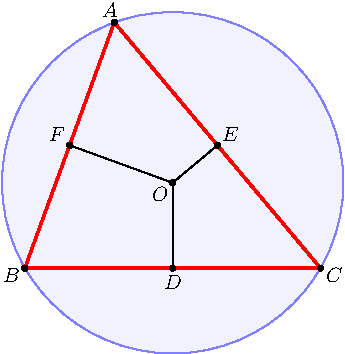
\includegraphics{circum.pdf}
\caption{Circumcenter of \(\triangle ABC\)}
\end{figure}
The proof of concurrency is very easy. Just remember that any point on the perpendicular bisector is equidistant from two of the corresponding vertex. 
%He showed the proof of concurrency of the perpendicular bisector of the sides of a triangle. I am not going to include the proof as you can find it in anywhere. 

\section{Centroid}

Centroid is the intersection of the medians of a triangle. It is defined by \(G\). It is also called Center of Mass or Center of Gravity.
\begin{figure}[h]
	\centering
	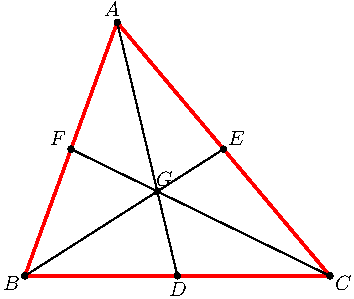
\includegraphics{centroid.pdf}
\caption{Centroid of \(\triangle ABC\)}
\end{figure}


Here we are going to see a combinatorial proof!

Let, three centroid don't concur, then they intersect in three pints let \(G_1,G_2,G_3\). Let 
the midpoints of the sides are \(L,M,N\). Then draw the medians of the triangle \(LMN\) then, 
their medians intersect at \(G_1,G_2,G_3\) as \(MN\parallel BC\). So we are going to infinite 
descent, and consider the median triangle of \(LMN\). Consequently, the areas of the median 
triangles are going to \(0\). But the area of triangle \(G_1G_2G_3\) remains same. which means 
triangle \(G_1G_2G_3\) is bigger that the original triangle which is a contradiction. So 
centroid exists. 


\section{Orthocenter}

Let \(D,E,F\) be the foot of the perpendicular from \(A,B,C\) to the opposite side of the 
triangle. Then \(BFEC\) is a cyclic quadrilateral(You can see this by \(\angle FEA = B\) or by 
\(\angle BFC = \angle BEC =90\dg\)). Also there are another two cyclic quadrilaterals. Find them.


\begin{figure}[ht]
%\centering
\begin{center}
	\begin{minipage}[t]{6.5cm}
		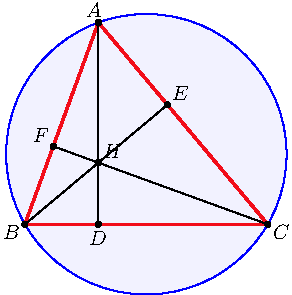
\includegraphics{ortho.pdf}
	\\ \centering \sffamily Orthocenter of \(\triangle ABC\)
	\end{minipage}
		\quad
	\begin{minipage}[t]{6.5cm}
		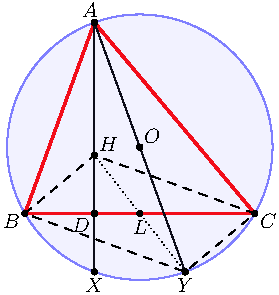
\includegraphics{ortho-reflect.pdf}
	\\ \centering \sffamily Reflection of Orthocenter lies on Circumcirlce
	\end{minipage}
\end{center}	
\caption{Ortocenter and its Reflections}
\end{figure}

There are six cyclic quadrilaterals and the orthocenter is the incenter of the orthic trinagle.


\begin{figure}[ht] 
\centering
		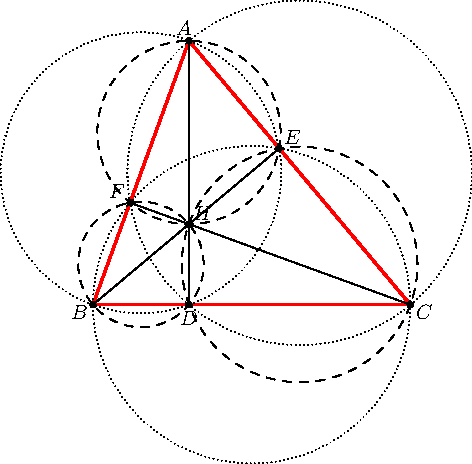
\includegraphics{ortho-6cyclic.pdf}
\caption{Orthocenter and 6 cyclic quadrilaterals}
\end{figure}

Then Mentor taught us the reflection of the orthocenter across the sides and about the midpoint of the sides lie on the circumcircle of the triangle \(ABC\). 
Let the reflection of \(H\) across the side \(BC\) is \(X\) then we are going to show that \(X\) lies on \((ABC)\). 

Note that \(\triangle BDH \cong \triangle BDX\) by some angle chasing.

So, \(\angle BXH = \angle BHD = \angle ACB\) and therefore \(ABXC\) is a cyclic quadrilateral.

Let the reflection of H acroos the midpoint of \(BC\) is \(Y\).
Then, \[\angle BAH = \angle CAO=90\dg - B.\]
and \(AY\) is a diameter.

\(BH=CY\) hence, \(BH\parallel CY\) thererfore, \(BHCY\) is a parallelogram, and \(H,L,Y\) are collinear. hence \(Y\) lies on \((ABC)\).




\section{Nine Point Circle}
Our current topic is the famous Nine-Point Circle whih goes through exactly nine points.

These pints are three midpoints, three feet of the perpendicular and the three midpoints of \(AH,BH,CH\).

Now we are going to show the first six points are concyclic.
%npc
\begin{figure}[ht] 
\centering
		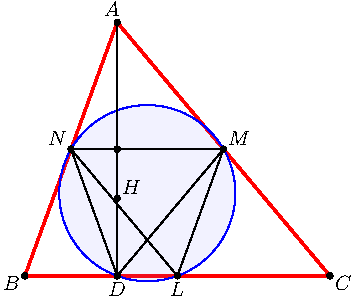
\includegraphics{npc-proof.pdf}
\caption{\(D,L,M,N\) lie on a circle}
\end{figure}
\(D\) is the reflection of \(A\) across \(MN\)
so \(\angle MDN = A\) we also know that \(\angle MLN = A\) so \(L,M,N,D\) are concyclic . Similarly we can show that \(L,M,N,E\) and \(L,M,N,F\) are concyclic, so all six points are concyclic.
Other proof \(\angle BDN = \angle NML\) so \(L,M,N,D\) are concyclic points.


Now we are gonna prove that \(K\) the midpoint of \(AH\) lies on \((DEFLMN)\). 
\(\angle NLB = C \) so we have to show that \(\angle NKH = C\). but \[ \angle NKH= \angle BHD = C\] so we are done.

Also \(N_9\) the center of the Nine-Point Circle is the midpoint of \(OH\) where \(O\) and \(H\) are circumcenter and Orthocenter respectively.

%npc
\begin{figure}[ht] 
\centering
	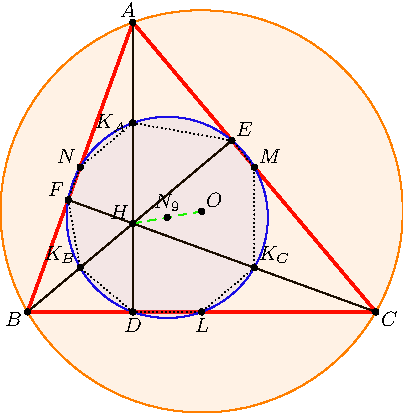
\includegraphics{npc-full.pdf}
\caption{Nine Point Circle of \(\triangle ABC\)}
\end{figure}


\section{Practice Problems}

\begin{problem}
Let $H$ be the orthocenter of triangle $ABC$ and $D,E,F$ be the feet of the perpendicular on the sides $BC,CA,AB$. Prove that $H$ is the incenter of triangle $DEF$.
	\begin{hint}
		\addhint{ }
		\addhint{ }
		%\addhint{Solution at \url{}}
	\end{hint}
\end{problem}

\begin{problem}
Prove that the reflection of the \textit{Euler Line} on the sides of $\triangle ABC$ concur at the circumcircle.
	\begin{hint}
		\addhint{ }
		\addhint{ }
		%\addhint{Solution at \url{}}
	\end{hint}
\end{problem}

\begin{problem}[2020 China North Mathematical Olympiad (Basic) P4]
In $\triangle ABC$, $\angle BAC = 60^{\circ}$, point $D$ lies on side $BC$, $O_1$ and $O_2$ are the centers of the circumcircles of $\triangle ABD$ and $\triangle ACD$, respectively. Lines $BO_1$ and $CO_2$ intersect at point $P$. If $I$ is the incenter of $\triangle ABC$ and $H$ is the orthocenter of $\triangle PBC$, then prove that the four points $B,C,I,H$ are on the same circle.
	\begin{hint}
		\addhint{ }
		\addhint{ }
		\addhint{Solution at \url{https://artofproblemsolving.com/community/c6h2220889p16882243}}
	\end{hint}
\end{problem}

\begin{problem}[Swiss MO 2007/4]
Let $ABC$ be an acute-angled triangle with $AB> AC$ and orthocenter $H$. Let $D$ the projection of $A$ on $BC$. Let $E$ be the reflection of $C$ wrt $D$. The lines $AE$ and $BH$ intersect at point $S$. Let $N$ be the center of $AE$ and let $M$ be the midpoint of $BH$. Prove that $MN$ is perpendicular to $DS$.
	\begin{hint}
		\addhint{ }
		\addhint{ }
		\addhint{Solution at \url{https://artofproblemsolving.com/community/c6h2197471p16518225}}
	\end{hint}
\end{problem}

\begin{problem}[British MO 1981 P1]
$H$ is the orthocentre of triangle $ABC$. The midpoints of $BC, CA, AB$ are $A', B', C'$ respectively. A circle with centre $H$ cuts the sides of triangle $A'B'C'$ (produced if necessary) in six points, $D_1, D_2$ on $B’C'$,$E_1, E_2$ on $C'A'$ and $F_1, F_2$ on $A'B'$. Prove that, $AD_1=AD_2=BE_1=BE_2=CF_=CF_2$.
	\begin{hint}
		\addhint{ }
		\addhint{ }
		\addhint{Solution at \url{https://artofproblemsolving.com/community/c6t70430f6h2531807_ad_1ad_2be_1be_2cf_cf_2_wanted_circle_center_h_through_6_points}}
	\end{hint}
\end{problem}

\begin{problem}[47th Austrian MO P2]
We are given an acute triangle $ABC$ with $AB > AC$ and orthocenter $H$. The point $E$ lies symmetric to $C$ with respect to the altitude $AH$. Let $F$ be the intersection of the lines $EH$ and $AC$. Prove that the circumcenter of the triangle $AEF$ lies on the line $AB$.
	\begin{hint}
		\addhint{ }
		\addhint{ }
		\addhint{Solution at \url{https://artofproblemsolving.com/community/c6h1681663p10722184}}
	\end{hint}
\end{problem}

\begin{problem}
Let $ABC$ be an acute triangle with orthocenter $H$ and circumcenter $O$. Let $K$ be the midpoint of the segment $AH$. Let $P$ be a point on $AC$ such that, $OP \parallel BC$. Show that $\angle BKP= 90^{\circ}$ 
	\begin{hint}
		\addhint{ }
		\addhint{ }
		\addhint{Solution at \url{https://artofproblemsolving.com/community/q1h2353259p19090174}}
	\end{hint}
\end{problem}

\begin{problem}[2017 Saudi Arabia JBMO TST P7]
Let $ABC$ be a triangle inscribed in the circle $(O)$, with orthocenter $H$. Let d be an arbitrary line which passes through $H$ and intersects $(O)$ at $P$ and $Q$. Draw diameter $AA'$ of circle $(O)$. Lines $A'P$ and $A'Q$ meet $BC$ at $K$ and $L$, respectively. Prove that $O, K, L$ and $A'$ are concyclic.
	\begin{hint}
		\addhint{ }
		\addhint{ }
		\addhint{Solution at \url{https://artofproblemsolving.com/community/c6h2124972p15486860}}
	\end{hint}
\end{problem}

\begin{problem}[2019 Romania JBMO TST Day 2 P3]
Let $d$ be the tangent at $B$ to the circumcircle of the acute scalene triangle $ABC$. Let $K$ be the orthogonal projection of the orthocenter, $H$, of triangle $ABC$ to the line $d$ and $L$ the midpoint of the side $AC$. Prove that the triangle $BKL$ is isosceles.
	\begin{hint}
		\addhint{ }
		\addhint{ }
		\addhint{Solution at \url{https://artofproblemsolving.com/community/c6h2135307p15639880}}
	\end{hint}
\end{problem}

\begin{problem}[Ukraine TST 2014 p4]
The $A$-excircle of the triangle $ABC$ touches the side $BC$ at point $K$. The circumcircles of triangles $AKB$ and $AKC$ intersect for the second time with the bisector of angle $A$ at points $X$ and $Y$ respectively. Let $M$ be the midpoint of $BC$. Prove that the circumcenter of triangle $XYM$ lies on $BC$.
	\begin{hint}
		\addhint{ }
		\addhint{ }
		\addhint{Solution at \url{https://artofproblemsolving.com/community/c6h2082814p14992490}}
	\end{hint}
\end{problem}

\begin{problem}[2020 Nicaragua Iberoamerican MO TST]
Let $H$ and $O$ be the orthocenter and circumcenter of an scalene and acute-angled triangle $ABC$ with circumcircle $\Gamma$. Points $K$ and $M$ are the midpoints of $AH$ and $BC$, respectively. Let $L$ be a point on the circumcircle of $OAK$ so that $\angle ALM=90^{\circ}$.\\
    
If line $AO$ meets $\Gamma$ again at $D$, and line $AL$ meets $\Gamma$ again at $J$, show that $MD$ and $DJ$ are perpendicular to each other.
	\begin{hint}
		\addhint{ }
		\addhint{ }
		\addhint{Solution at \url{https://artofproblemsolving.com/community/c6h1993208p13898771}}
	\end{hint}
\end{problem}

\begin{problem}[2020 Estonia TST P4]
Let $O$ be the circumcenter and $H$ the orthocenter of an acute-triangle $ABC$. The perpendicular bisector of $AO$ intersects the line $BC$ at point $S$. Let $L$ be the midpoint of $OH$. Prove that $\angle OAH = \angle  LSA$.
	\begin{hint}
		\addhint{ }
		\addhint{ }
		\addhint{Solution at \url{https://artofproblemsolving.com/community/q1h2292197p18049462}}
	\end{hint}
\end{problem}

\begin{problem}[2016 Thailand TST Day 1 P1]
Let $\vartriangle ABC$ be an acute-angled triangle whose altitudes $AA_1$ and$ BB_1$ intersect at $H$. Let $\omega_1$ be the circle centered at $H$ passing through $B_1$ and let $\omega_2$ be the circle centered at $B$ passing through $B_1$. Let $CN$ and $CK$ be the tangent lines from $C$ to circles $\omega_1$ and $\omega_2$ respectively ($N$ and $K$ are distinct from $B_1$). Prove that $A_1, N$ and $K$ are collinear.
	\begin{hint}
		\addhint{ }
		\addhint{ }
		\addhint{Solution at \url{https://artofproblemsolving.com/community/c6h2315798p18441752}}
	\end{hint}
\end{problem}

\begin{problem}[USA TST 2011 P1]
In an acute scalene triangle $ABC$, points $D,E,F$ lie on sides $BC, CA, AB$, respectively, such that $AD \perp BC, BE \perp CA, CF \perp AB$. Altitudes $AD, BE, CF$ meet at orthocenter $H$. Points $P$ and $Q$ lie on segment $EF$ such that $AP \perp EF$ and $HQ \perp EF$. Lines $DP$ and $QH$ intersect at point $R$. Compute $HQ/HR$.
	\begin{hint}
		\addhint{ }
		\addhint{ }
		\addhint{Solution at \url{https://artofproblemsolving.com/community/c6h420422p2374795}}
	\end{hint}
\end{problem}

\begin{problem}[Canadian Buffet Contest 2021 G4]
In $\triangle ABC$, let $D$, $E$, $F$ be the feet of altitudes from $A$, $B$, $C$ respectively. Let $K$ be the orthocenter of $\triangle DEF$. Let $U$,$V$,$W$ be the projections of points $F$, $D$, $E$, on $BC$, $CA$, $AB$ respectively. Assume that the circumcircles of $\triangle ABC$ and $\triangle UVW$ intersect at two points $M$ and $N$, prove that $KM=KN$.
	\begin{hint}
		\addhint{ }
		\addhint{ }
		\addhint{Solution at \url{https://artofproblemsolving.com/community/c6t70430f6h2538253_on_the_properties_of_orthocenter_of_def}}
	\end{hint}
\end{problem}

\begin{problem}[Iran MO 3rd round 2018 G4]
For acute triangle $\triangle ABC$ with orthocenter $H$, and $E,F$ the feet of altitudes for $B,C$, we have $P$ on $EF$ such as that $HO \perp HP$. $Q$ is on segment $AH$ so $HM \perp PQ$. prove $QA=3QH.$
	\begin{hint}
		\addhint{ }
		\addhint{ }
		\addhint{Solution at \url{https://artofproblemsolving.com/community/c6t70430f6h1701020_iran_geometry_third_round_2018}}		
	\end{hint}
\end{problem}
%\section{}

%\includepdf[pages=-]{triangle-center-pset.pdf}

%\begin{soln}[to Problem 1.1]
%This is trivial. Just angle Chase.
%\end{soln}





\chapter{Basic Divisibility}% by Zim-mim Siddiqee Sowdha}
\label{sec:divi}

\begin{linkb}
   \begin{itemize}
        \item \href{https://www.youtube.com/watch?v=2LoYjvi0MH4}{Basic Divisibility (Sowdha)}
        \item \href{https://drive.google.com/file/d/1YRvC4AQ2rwa4DsQxYd_7kHqyYZdrPQkX/view?usp=sharing}{Basic Number Theory - Masum Billal}
   \end{itemize}
\end{linkb}

\section{Basic Divisibility}
For all integers \(a\), \(1|a\). 

\paragraph{Divisibility Properties}
\begin{itemize}
	\item \(a|b\) then there exist a inetger \(k\) s.t \(b=ak\).
	\item \(a|b, a|c \implies a | b \pm c\)
	\item \(a|b \implies a | bc\)
	\item \(a|b, b|a \implies a=b\)
	\item \(m|(a-b), m|(c-d) \implies m|(ac-bd)\). by \(m|(a-b)c-(c-d)b=ac-bd \)
\end{itemize}

\section{Division Algorithm}
This is one of the most famous topic. It tells that if \(a, b \in \mathbb{Z}\) then there exists unique \(q,r\)
s.t \[a=bq+r; \ \ \ \ 0\le r<|b|\]



\section{Fundamental Theorem of Arithmetic (FTA)}
Every integer has an unique prime power factorization which is called the Fundamental Theorem of Arithmetic.
\[ N ={p_1}^{a_1} {p_2}^{a_2} {p_3}^{a_3} \cdots {p_m}^{a_m}. \]

Let assume that, the factorization is not unique. Then we have, 
\[ N ={p_1}^{a_1} {p_2}^{a_2} {p_3}^{a_3} \cdots {p_m}^{a_m} ={q_1}^{b_1} {q_2}^{b_2} {q_3}^{b_3} \cdots {q_n}^{b_n}. \]

Now we have,
\[p_1 | q_1 q_2 q_3 \cdots q_n\]
\[\implies p_1 | q_i\]
By Euclid's Lemma \[p_i = q_i\]

If $m\neq n$ then $1=q_x q_y q_z$ for some $x,y,z$ which is a contradiction.

\section{Modular Arithmetic}

Modular Arithmetic means working with remainders where remainders aren't fixed. 
\begin{enumerate}
	\item \textbf{Congruence:}
		$m|a-b \implies a \equiv b \pmod m$.
	\item $a$ is divided by $m$ and remanider is $b$ then $a\equiv b \pmod m$.
	\item $a=bq+r \implies a\equiv r \pmod b.$
%	\item 
\end{enumerate}

\paragraph{Some Properties of Modular Arithmetic}
\begin{enumerate}
	\item $a\equiv b \pmod m \implies a+mx \equiv b+my \pmod m .$
	\item $a\equiv b \pmod m; c \equiv d \pmod m \implies a \pm c \equiv b \pm d \pmod m .$
	Also $ ka \equiv kb \pmod m .$
	\item $a\equiv b \pmod m; c \equiv d \pmod m \implies ac \equiv bd \pmod m.$
	Which means $a^k \equiv b^k \pmod m$ which is very useful.
	\item $ak \equiv bk \pmod m \mathrm{and} (m,k)=1 \implies a \equiv b\pmod m.$
\end{enumerate}

\begin{example}
$7^{259} \equiv m \pmod 5 .$ Find $m$.
\end{example}

\begin{soln}
$$7^2 \equiv 2^2 \equiv 4 \equiv -1 \pmod 5$$ $$ (7^2)^{129} \equiv (-1)^{129} \equiv -1 \pmod 5 $$
$$ 7^{259} \equiv -7 \equiv -7+10 \equiv 3 \pmod 5 $$.
\end{soln}

\section{Residue Class/System Modulo $m$}
$n$ is an integer. $n$ divided by $6$ we can get $6$ residue. They are $0,1,2,3,4,5$. This set is called Residue system modulo $6$.
Let $S$ be the set, then \[ S=\{0,1,2,3,4,5 \} \equiv \{0,1,8,3,4,-1\} \pmod 6 .\]

The set is defined by $RS_{(m)}$

And as an example, \[RS_{(12)} =\{0,1,2,3,\ldots , 11\}\]

Note that here $1,5,7,11$ are coprime to $12$ and if we consider this set of \(\{1,5,7,11\}\) which is called as reduced Residue System modulo $12$.

\[RRS_{(12)}=\{1,5,7,11\}\]

$\varphi (m) $ is called the Euler's Totient Function and it is the number of elements in the set $RRS_{(m)}$. As an example $RRS_{(12)}=4$.

For prime $p$ we have $\varphi (p) =p-1$.

\begin{theorem}[Euler's Theorem]
For any integer $a$ coprime to $m$, we have, \[a^{\varphi (m)} \equiv 1 \pmod m \].
Which also means that \( a^{p-1} \equiv 1 \pmod p \).
\end{theorem}


Here is Fermat's Little Theorem. It comes from Euler's phi function.

\begin{theorem}[Fermat's Little Theorem]
Let $a$ be a positive integer and $p$ be a prime then, \[ a^p \equiv a \pmod p.\]
\end{theorem}

\section{Practice Problems}


\begin{problem}
Find all $d \in \mathbb{Z}^+$ such that $d$ divides $n^2+1$ and $(n+1)^2+1$ for some $n \in \mathbb{N} $
	\begin{hint}
		\addhint{Use $d|2n+1$ and $d|n^2+1$. try to transform them and then subtract.}
		\addhint{ }
	\end{hint}
\end{problem}


\begin{problem}
Find the maximum value of $x$ such that $x + 25 | (x + 2)^2$
	\begin{hint}
		\addhint{ Homogenize both ends and then subtract to isolate $x$ on one end and a constant on the other.}
		\addhint{ }
	\end{hint}
\end{problem}


\begin{problem}
Show that $2^{32}+1$ is divisible by $641$.
	\begin{hint}
		\addhint{Use $a\equiv b \pmod m; c \equiv d \pmod m \implies ac \equiv bd \pmod m.$ }
		\addhint{ }
	\end{hint}
\end{problem}

\begin{problem}
Prove that if $m|n$ then $a^m-1 | a^n -1$  
	\begin{hint}
		\addhint{$a^{xy}=(a^x)^y $}
		\addhint{ }
	\end{hint}
\end{problem}

\begin{problem}
Prove that for all odd $k \in \mathbb{N}$ -

\begin{center}
$1+2+ . . .+n|1^k+2^k+. . . + n^k$
\end{center}
	\begin{hint}
		\addhint{$1+2+ . . .+n= \frac{n(n+1)}{2} $ }
		\addhint{$1+(n-1)|i^k+(n-i)^k$ and $n+1|(i)^k+(n-i+1)^k$    }
	\end{hint}
\end{problem}

\begin{problem}
Find all n such that
\begin{center}
$44 ... 44$ ($n$ times $4$)
\end{center}
is a perfect square.

	\begin{hint}
		\addhint{Look in mod 4}
		\addhint{ }
	\end{hint}
\end{problem}

\begin{problem}
Find all $n \in \mathbb{N} \cup \{0\} $ such that, $2^n+n | 8^n +n$
	\begin{hint}
		\addhint{$a + b|a^3 + b^3$ }
		\addhint{Prove that $n \in [1,9]$ }
	\end{hint}
\end{problem}

\begin{problem}
Find all positive integer solutions to the equation, $2^n-1=3^m$
 
	\begin{hint}
		\addhint{ }
		\addhint{ }
	\end{hint}
\end{problem}

\begin{problem}
Show that if $x^3+y^3=z^3$ then one of $x,y,z$ is divisible by $7$ 
	\begin{hint}
		\addhint{Use the set of cubic residues of mod 7}
		\addhint{ }
	\end{hint}
\end{problem}


\chapter{Induction}% by Muhaiminul Islam Ninad}

\begin{linkb}
   \begin{itemize}
        \item \href{https://www.youtube.com/watch?v=C-0pRTD4H0w}{Induction (Ninad)} 
        \item \href{https://drive.google.com/file/d/1Z1h4jfZvrb69Jrayc0IMmopX9yzz9Z_L/view?usp=sharing}{First} \(+\) \href{https://drive.google.com/file/d/12zWftwXBXeYKMCBMGh-cPhG69r0zoc99/view}{Second}
   \end{itemize}
\end{linkb}

Today's Topic is Basic Induction. Our mentor started with showing an inductive proof of sum of positive integers:
\[ 1 + 2 +3+ \ldots + n = \frac{n(n+1)}{2} .\]
It is easy and left as an exercise.

\section{Induction/Weak Induction}
Our next problem is:

\begin{example}
Let, \(a_1=\sqrt{2}, a_{i+1}=\sqrt{2+a_i}\). Prove that, \[ a_n = 2\cos \frac{\pi}{2^{n+1}}. \]
\end{example}

\begin{soln}
Here we show that, base case is true as \(a_1=2\cos \frac{\pi}{2^2} = 2\cos \frac{\pi}{4} =2 \cdot \frac{1}{\sqrt 2} = \sqrt{2} \).

Now assume that it is true for \(a_k\) and \(a_k=2\cos \frac{\pi}{2^{k+1}}\). Then we will show that \(a_{k+1} = 2\cos \frac{\pi}{2^{k+2}}\).

\end{soln} 


\begin{example}
Show that for all positive integer \(n\), \[ 1+ \frac{1}{\sqrt{2}}+ \frac{1}{\sqrt{3}}+ \frac{1}{\sqrt{4}}+ \ldots \frac{1}{\sqrt{n}} \le 2\sqrt{n}. \]
\end{example}

\begin{soln}
Here, after showing the base case true, assume that it's true for integer $k$. Then for $k+1$, add $\frac{1}{\sqrt{k+1}}$ to both side.

After these, show that, $2\sqrt{k} + \frac{1}{k+1} \le 2\sqrt{k+1}$
Done!
\end{soln}

\begin{example}
Prove that for all positive integer \(n\), 
\[ \frac{1}{2} \cdot  \frac{3}{4} \cdot  \frac{5}{6} \cdot \cdots  \frac{2n-1}{2n} < \frac{1}{\sqrt{3n}} .\]
\end{example}

\begin{soln}
Here assume that it's tru for $k-1$ then show for $k$.

Then do some algebra which is left as exercise!
\end{soln}


\section{Strong Induction}
In this tecknique, we will assume that the statement is true for all integers from base case to \(k\) (in general).
Then we will show that its true for \(k+1\), and often we use the assertion that the statement is true for all integers from base case to \(k\).

\begin{example}
%Prove that any positive integer can be written as the sum of distinct and non-consecutive one or more Fibonacci Numbers.
The Fiobonacci sequence is defined as $F_1 = 1, F_2 = 2$ and for $n \ge 1$,
$F_{m+2} = F_{m+1} + F_m$. Show that every natural number n can be written as a sum of distinct
fiobonacci numbers, with no $2$ Fiobonacci numbers being consecutive ($F_n$ and $F_{n+1}$ are
consecutive).
\end{example}
%Note that Fibonacci numbers are \(F_1=1, F_2 = 1 , F_3 =3, \ldots F_n=F_{n-1} + F_{n-2} \).
\begin{soln}
We proceed by strong induction. Let $P(n)$ be the statement that n can be written
as a sum of distinct fiobonacci numbers with no $2$ consecutive. It is easy to verify $P(1)$
and $P(2)$. We now proceed by strong induction, so assume $P(i)$ for all $1 \le i \le n$. Now
consider the number $n + 1$ and the highest $F_m$ such that $F_m \le n + 1$. Then if $n + 1 = F_m$ we are done.
Otherwise, $n + 1 - F_m$ is a positive integer less than $n + 1$, and so $P(n + 1 - F_m)$ is
true by assumption. Therefore, we can write $n + 1 - F_m = F_{i_1} + F_{i_2} + \dots + F_{i_k}$ for distinct Fiobonacci numbers, no $2$ of which are consecutive. Now we have written $n + 1$ as a sum of distinct fiobonacci numbers
\[ n + 1 = F_{i_1} + F_{i_2} + \ldots + F_{i_k} + F_m.\]
such that no $2$ are consecutive execpt possibly the largest $2$, if $F_{i_k} = F_{m-1}$. But the latter case would imply that $n \le F_m + F_{m-1} = F_{m+1}$, contradicting the choice of $m$. This completes the induction.
\end{soln}
The above soln is from Jacob Tsimerman's \textit{A closer look at Induction} note.




\section{Real Induction}
\begin{example}
There are \(n\) lamps in a room, with certain lamps connected by wires. Initially
all lamps are off. You can press the on/off button on any lamp \(A\), but this also switches
the state of all the lamps connected to lamp \(A\) from on to off and vice versa. Prove that
by pressing enough buttons you can make all the lamps on. (Connections are such that if
lamp \(A\) is connected to lamp \(B\), then lamp \(B\) is also connected to lamp \(A\).)
\end{example}

\begin{soln}
We use induction on n. The base case of \(n = 1\) is trivial (just turn the lamp on).
Now assume the case of \(n - 1\) lamps. Now look at the set of n lamps and ignore some
lamp \(A\). Then by induction, we can turn the remaining lamps on by pressing the buttons
on some subset of them. Now if at the end of doing this \(A\) is also on, we are done. So we
can assume that at the end of doing this \(A\) is off. Since \(A\) was an arbitrary lamp, we can
assume that by pressing a sequence of buttons we can flip the states of all lamps except
one of our choosing. Now, taking \(A\) and \(B\) to be 2 different lamps and flipping the states
first of all lamps different from \(A\) and then all lamps different from B, we see that we can
flip the states of only \(A\) and \(B\). So this means we can flip the states of any number of even
lamps. Now we have 2 cases:
\begin{itemize}
	\item \(n\) is even: Then we are already done, since we can flip the states of any number of
even lamps.
	\item \(n\) is odd: In this case, there must be some lamp A connected to an even number of
lamps (prove this!) so first press the button on lamp \(A\). Now, including \(A\), an odd
number of lamps are on, so an even number of lamps that are off remain. Flip their
states to finish the proof!
\end{itemize}

\end{soln}
The above solution is from Jacob Tsimerman's \textit{A closer look at Induction} note.

Our class ended!

%\begin{problem}

%\end{problem}



\section{Practice Problems}


\begin{problem}

	\begin{hint}
		\addhint{ }
		\addhint{ }
	\end{hint}
\end{problem}

\begin{problem}

	\begin{hint}
		\addhint{ }
		\addhint{ }
	\end{hint}
\end{problem}

\begin{problem}

	\begin{hint}
		\addhint{ }
		\addhint{ }
	\end{hint}
\end{problem}

\begin{problem}

	\begin{hint}
		\addhint{ }
		\addhint{ }
	\end{hint}
\end{problem}

\begin{problem}

	\begin{hint}
		\addhint{ }
		\addhint{ }
	\end{hint}
\end{problem}

\begin{problem}

	\begin{hint}
		\addhint{ }
		\addhint{ }
	\end{hint}
\end{problem}

\begin{problem}

	\begin{hint}
		\addhint{ }
		\addhint{ }
	\end{hint}
\end{problem}


\begin{problem}

	\begin{hint}
		\addhint{ }
		\addhint{ }
	\end{hint}
\end{problem}


\chapter{Invariants and Monovariants}% by Raiyan Jamil}
\label{sec:inv-mono}

\begin{linkb}
   \begin{itemize}
        \item \href{https://www.youtube.com/watch?v=hInrF3biygw}{Invariants (Raiyan)}
        \item \href{https://drive.google.com/file/d/1Ndgs_ftSaG1Ph5sJYsIbwgGczM_NNgrW/view}{Class Note}
        \item \href{https://drive.google.com/file/d/15XjviqGWzT3T_7-W7g2axDdOXiE2le8K/view}{Invariants and Monovariants}
   \end{itemize}
\end{linkb}

This topic covers the trick of Invariant and Monovariants which are very powerful weapons to tackle hard combinatorial problems. 

Invariant means which doesn't change after some steps or operations. 

Monovariants means the value changes only in one direction, either it increases or decreases.

\section{Invariants}

\begin{example}
You have an equilateral triangle. In each "step", you can:
	\begin{itemize}
		\item Draw a line on the current shape and cut it into two pieces along the line.
		\item Then flip one of the pieces and join the two pieces again along the line.
	\end{itemize} 
\end{example}

\begin{figure}[h!]
\centering
		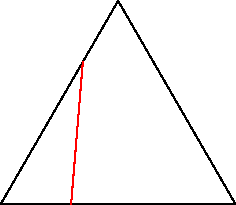
\includegraphics{equi-tri.pdf}
\end{figure}

\begin{soln}
After some move you may realize that, the perimeter and the area of the shape remains same as initial position.

SO if we want to make it a square then let the sise length of the square is $x$, and the length of the side of the equilateral triangle is $a$, so w havefollowing two equation:
\[\frac{\sqrt 3}{4}a^2 = x^2\]
\[3a = 4x.\]
which have no common solution. So it is not possible to make it a square.

\end{soln}


\begin{example}
In an empty room, in every minute either $4$ people enter or $3$ people leave. Can there be $7^{125}+5$ people in the room after $7^{666}$ minutes?
\end{example}

\begin{soln}
The trick in htis problem is to work with mod $7$, per $7$ minutes.

Let ititially there are $x$ people in the room. So in $7$ minutes there let $4$ people inter $a$ times and $7-a$ people leave the room. So after seven minutes there are $x+4a -3(7-a)=x+7(a-3)$ people. This leads us to work with modulo seven.

As initially there are zero people in the room so $x \equiv 0 \pmod 7 $ but $7^{125}+5 \not\equiv 0 \pmod 7$ so the answer is no.
\end{soln}



\begin{example}
An $8\times 8$ chessboard has two opposite corners removed. Is it possible to tile the remaining $62$ squares with $31$ dominoes?
\end{example}

\begin{soln}
The answer is NO. Color the board with black-white. And there are $31$ black and $30$ white squares but the number of black and white squares should be the same for tiling.
\end{soln}



\begin{example}
In a cube there are seven vertices amrked $0$ and one marked $1$. It is permitted to add $1$ to any two neighbouring vertices (that is two vertices connected by edge). Is it possible that all the numbers are divisible by $3$ after a finite number of steps?
\end{example}

\begin{soln}
Here, the answer is also NO.

Alternately color the vertices with black and white. Then after each move we add 1 to white and 1 to black. Let $S_b$ and $S_w$ denote the sum of the numbers in Black and White vertices respectively. Then $S_b - S_w =1 $ remains constant as initially there was the sum 1. Which means it is not possible that all the numbers are divisible by three.
\end{soln}




\begin{example}
The numbers $1, 2, 3, \ldots ,n$ are written in a row. It is permitted to swap any two numbers. If 2007 such operations are performed, is it possible that the final arrangement of numbers coincides with the original.
\end{example}

\begin{soln}
The answe is NO.

Here we define \textit{inversion} which is the number of such pair of consecutive elements in the row such that for $x,y$ the sequence:
\[1, 2, 3, \ldots ,y, x, \ldots ,n\]
$y$ is left to $x$ and $y>x$.

Now you can observe that after each move inversion can increase or decrease by $1$.

Initially there was inversion=0, but after 2007 move the inversion will be odd. So it is not possible.
\end{soln}



\begin{example}
A natural number is written in each square of an $m \times n$
chessboard. The allowed move is to add an integer $k$ to each of
two adjacent numbers in such a way that nonnegative numbers
are obtained (two squares are adjacent if they share a common
side). Find a necessary and sufficient condition for it to be
possible for all the numbers to be zero after finitely many
operations.
\end{example}

\begin{soln}
Note that in each move, we are adding the same number to 2
squares, one of which is white and one of which is black (if the
chessboard is colored alternately black and white). If $S_b$ and $S_w$
denote the sum of numbers on black and white squares
respectively, then $S_b - S_w$ is an invariant. Thus if all numbers are 0
at the end, $S_b - S_w = 0$ at the end and hence $S_b - S_w = 0$ in the
beginning as well. This condition is thus necessary; now we prove
that it is sufficient.

Suppose $a, b, c$ are numbers in cells $A, B, C$ respectively, where
$A, B, C$ are cells such that $A$ and $C$ are both adjacent to $B$. If $a \le b$,
we can add $(-a)$ to both $a$ and $b$, making $a \ 0$. If $a \ge b$, then add $(a-b)$
to $b$ and $c$. Then $b$ becomes $a$, and now we can add $(-a)$ to both of
them, making them $0$. Thus we have an algorithm for reducing a
positive integer to $0$. Apply this in each row, making all but the
last 2 entries 0. Now all columns have only zeroes except the last
two. Now apply the algorithm starting from the top of these
columns, until only two adjacent nonzero numbers remain. These
last two numbers must be equal since $S_b = S_w$ . Thus we can reduce
them to 0 as well.
\end{soln}




\section{Monovariants}

\begin{example}
Several positive integer numbers are written on a blackboard. One can erase any two distinct integers and write their greatest common divisor and least common multiple instead.
\begin{enumerate}[(a)]
	\item Prove that eventually the numbers will stop changing.
	\item Prove that the values of the numbers, once they stop changing, do not depend on what moves were made.
\end{enumerate}
\end{example}

\begin{soln}
For (a) observe that gcd and lcm increasing or decreasing (why?). By playing with numbers you will find a mnovariant. 
The rest is left as an execise.
\end{soln}





\begin{example}[Stanford Putnam Training 2007]
On an $n\times n$ board, there are $n^2$ squares, $n-1$ of which are infected. Each second, any square that is adjacent to at least two infected squares becomes infected. Show that at least one square always remains uninfected.
\end{example}

\begin{soln}
Left as an exercise!
\end{soln}



\section{Practice Problems}

\paragraph{Invariants}

\begin{problem}
Bobby is playing with a few pieces of paper. At each step, he takes one piece and 
then cuts it into $9$ or $13$ pieces. Initially he has only one piece of paper. Is it 
possible for him at some point to have exactly $2019$ pieces?
	\begin{hintone}
	\addhint{The answer is no. }
	\end{hintone}
\end{problem}

\begin{problem}
The numbers $1,0,1,0,0,0$ are written around a circle. At each step, you can take 
two adjacent numbers and add $1$ to both of them. Can you turn all the six numbers 
equal after a finite number of steps?
	\begin{hintone}
	\addhint{The answer is no. }
	\end{hintone}
\end{problem}

\begin{problem}
In a strange planet, there are three types of Chameleons of {\color{red} Red}, {\color{blue} Blue} and {\color{green} Green} 
colours respectively. At any point, if two Chameleons of different colours look at 
each other, they both change to the third colour. Initially, there are $100$ red, $200$ 
blue and $300$ green coloured Chameleons. Is it possible for all the Chameleons to 
turn into the same colour at some point in time?
	\begin{hintone}
	\addhint{ }
	\end{hintone}
\end{problem}

\begin{problem}
You have a $4 \times 4$ grid. In this box, there are $15$ cells with number $1$ in them and 
one cell with $-1$ in it. In each step, you can take any row or any column and then 
multiply the four numbers in that row or column by $-1$. Prove that, no matter 
how many times you do this, there will always be at least one $-1$ in the grid. 
	\begin{hintone}
	\addhint{ }
	\end{hintone}
\end{problem}

\begin{problem}
In an infinite grid, initially there are 4 stones on (0,0). At each step, you can take 
one stone from (m, n) and put one stone each on (m + 1, n) and (m, n + 1). Prove 
that at any point in time, we can always find a point on which there are at least 
two stones.
	\begin{hintone}
	\addhint{ }
	\end{hintone}
\end{problem}


\paragraph{Monovaiants}
\begin{problem}
You have $2n$ points on a plane. And there are $n$ line segments connecting pairs of 
points such that each point is the endpoint of exactly one segment. At each step, 
you take four points $A, B, C$ and $D$ such that $A$ and $B$ are connected and $C$ and $D$ are connected and $AB$ intersect $CD$. You then replace the two line segments 
$AB$ and $CD$ by $AC$ and $BD$. Prove that at some point there will be no more 
intersections.
	\begin{hintone}
	\addhint{Compute the sum of the lengths of the segments and observe that the sum is decreasing graduallly.}
	\end{hintone}
\end{problem}

\begin{problem}
Let $q$ be a rational number such that $0 \le q \le 1.$ Take the smallest positive integer 
$m$ such that $\frac{1}{m} \le q$ and then define $f (q) = q - \frac{1}{m}$. Show that, the sequence,
\[ f (q), f (f (q)), f (f (f (q))), \ldots \]
eventually becomes zero after finite number of steps.
	\begin{hintone}
	\addhint{The numbers in the sequences are rational numbers. Try comparing the numerators of the 
numbers.}
	\end{hintone}
\end{problem}

\begin{problem}[APMO 2019/2]
Let $m$ be a fixed positive integer. The infinite sequence $\{a_n\}$,  $n\ge 1$
is defined in the following way: $a_1$ is a positive integer, and for every integer $n \ge 1$,
we have,
\[ a_{n+1} = \begin{cases}
			a_n ^2 + 2^m & \text{ if } a_n < 2^m \\
			\frac{a_n}{2} & \text{ if } a_n \ge 2^m
		\end{cases} 
		\]
For each m, determine all possible values of a 1 such that every term in the sequence
is an integer.
	\begin{hintone}
	\addhint{For every number $a_i$ , consider the number $b_i$ to be its greatest odd divisor. Then find a property 
of $b_i$ and then derive a contradiction from that.}
	\end{hintone}
\end{problem}

\begin{problem}
There are $100$ rooms in a mansion and at a party $1000$ people were invited. After
each minute, if all of the people weren’t in the same room, exactly one person from
a room moves to another room which has a larger number of people in it. Prove
that, at some point, all the people will be in the same room.
	\begin{hintone}
	\addhint{Instead of taking the sum of size of the rooms, take the sum of squares of size of the rooms and
then see what happens after each minute.}
	\end{hintone}
\end{problem}

%\section{}



\chapter{Extremal Principle and Pigeonhole Principle}% by Nishat Anjum Bristy}

\begin{linkb}
   \begin{itemize}
        \item \href{https://www.youtube.com/watch?v=cYTssF84f9g}{Extremal and PHP (Bristy)}
        \item \href{https://drive.google.com/file/d/1sSvTee9gw9lAKwC0n6vyik79VrKpIiv6/view}{1}, \href{https://drive.google.com/file/d/17ps5RJ-FABW7CiSIj87zjC9de9FJyfn-/view}{2}, \href{https://drive.google.com/file/d/1_fbjgE7eFvVpFKNljJS24cN8NbPklCJu/view}{3}
   \end{itemize}
\end{linkb}

\section{Extreme Principle}
Every finite set has a least value and a greatest value. This is the basis of extreme principle.

As an example $\NN$ has the least value $1$.

Here is a motivating example of how to use extreme principle in Problem Solving.

\begin{example}
$n$ students are sitting in a field such 
that the distance between each pair of 
students is distinct. each student is 
holding a ball. When the teacher whistle, 
students throw their ball to the nearest 
student. Prove that there is a pair of 
students that throws their ball to each 
other.
\end{example}
Here starting with small values of $n$, we may guess the solution. The main idea is finding the least distance between two students. By extereme principle, there is a least distance betweeen two students. So, this $2$  students throw their balls to each other. Done!


\begin{example}
Find all the possible positive solutions to the equations.
\begin{align*}
x_1 + x_2 &= x_3 ^2 \\
x_2 + x_3 &= x_4 ^2 \\
x_3 + x_4 &= x_5 ^2 \\
x_4 + x_5 &= x_1 ^2 \\
x_5 + x_1 &= x_2 ^2
\end{align*}
\end{example}
Here you should guess the solution. You will find that $x_1=x_2=x_3=x_4=x_5=2$.

We will show that the solution must be equal to $2$, it can't be less that or grater that $2$.

By extremal principle, WLOG assume, $x_2$ is the least value here. So, we have,
\[ x_1 \le x_2, x_3, x_4, x_5\]
\[ x_1 \le x_4\]
\[ x_1 \le x_5\]
So, \[ 2x_1 \le x_4 +x_5 = x_1 ^2 \]
\[\implies x_1 \ge 2 \]

Similarly we can assume that $x_2$ is the greatest value here, and show that $x_2 \le 2$.

Then by the same argument, $x_3=x_4=x_5=x_1=x_2=2$.

So we are done.

\begin{example}
There are $n$ red points and $n$ blue points in a plane such that no three are collinear. Show that we can choose $n$  line segments so that, every line segment connects a red point with a blue point and no two line intersect . 
\end{example}
First, start with small values of $n$, you can find a monovariant here, that, if there is no intersections, then the sum of the lengths of the segments is least(by triangle inequality).

Let, assume a configuration with some intersections. Then, select an intersection, and then un-intersect it. In this process, we care about the sum of the lengths of the segments, by triangle inequality you can easily show that, with 4 points, if they intersects(2 line segments) then, in-intersect it and measure the sum, you can show that the last sum is obviously lesser than the previous.

It some point the sum become least. So we have to show that there is no intersection. Assume there is an inersection. Then using triangle inequality, there is a configuration with lesser sum, but we assumed the sum is least here. Contradiction!


\begin{example}
A finite set of points $S$ in a plane has the property that triangle determined by any thrree points in $S$ has area at most $1.$ Prove that, there exists a triangle with area $4$ that contains all the points
\end{example}
I am giving the solution with a diagram. :D 
\begin{figure}[h!]
\centering
	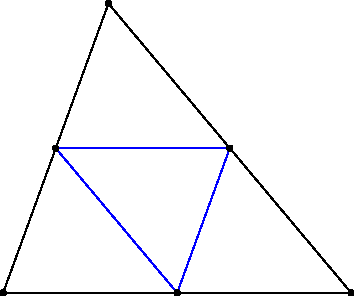
\includegraphics{php-tri.pdf}
	\caption{Guess the solution}
\end{figure}
%dont work


\section{Pigeonhole Principle}
Suppose there are $n$ pigeons to be placed within $n_1$ holes. Then you can easily say that there is hole which contains two pigeons. It is a trivial but very useful idea in solving combinatorial problems.
\begin{example}
A box has three pair of shocks colored red, blue and green. If the shocks are choosen without looking, at least how many shocks must be chosen to gurantee that at least one matching pair is there?
\end{example}
The answer is FOUR.


\begin{example}
Show that given a set of $n$ positive integers, there exists a non-empty subset where the sum of the elements is divisible by $n$.
\end{example}
Let, the set is $S=\{a_1, a_2, a_3, \dots , a_n \}$
And consider the following: 
\begin{align*}
s_1 &= a_1  \\
s_2 &= a_1+ a_2 \\
s_3 &= a_1, a_2, a_3 \\
\ldots \\
s_n &= a_1+ a_2+ \ldots + a_n
\end{align*}

$s_1, s_2, \ldots, _n$ may leave $n$ distinct residue modulo $n$ then one of them is $0$, done.

But if there are some two $s_i, s_j$ for which $s_i\equiv s_j \pmod n$ and $i<j$ then we have $s_j-s_i$ divisible by $n$.
\begin{example}
$10$ points are placed within an equilateral triangle of side length one. Show that, there exists two points with distance at most $\frac{1}{3}$ apart.
\end{example}
Look at the diagram. You may find the solution!
\begin{figure}[h!]
\centering
	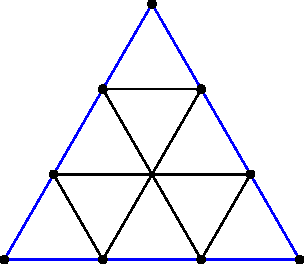
\includegraphics{php-tri-grid.pdf}
	\caption{There are nine triangle and ten points to be placed here!}
\end{figure}

Class ended!

\chapter{PoP, Radical Axis, Cyclic Quads}% by Raiyan Jamil}

\begin{linkb}
   \begin{itemize}
        \item \href{https://www.youtube.com/watch?v=iEilRQH6uL0}{POP, Radical Axis, Cyclic Quad (Raiyan)}
        \item \href{https://drive.google.com/file/d/1PlsMrV70QsknXCm5qDsRG5RIhLID_6rL/view}{(Zhao)} + \href{https://drive.google.com/file/d/1I53hLdluSuuN7O7Cuu4teubpSaxvwImZ/view}{POP} 
   \end{itemize}
\end{linkb}

What is Power of a Point? Well, its not the Microsoft Office's Power Point.  Its the most famous Power of a Point theorem which deals with a circle and a point. It tells that the power of a fixed point with respect to a fixed circle is constant. Let $P$ be a fixed point a circle be $\omega$ then,  let a line through $P$ intersects the circle at $A,B$ and another line through $P$ intersects the circle at $C,D$ respectively. Now, we have, 
\[ PA\cdot PB = PC \cdot PD.\]
which is called the Power of a Point.

\begin{figure}[ht]
\centering
		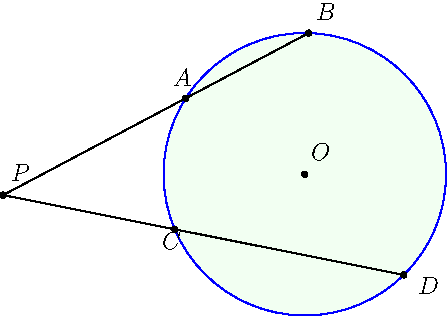
\includegraphics{pop-case1.pdf}
	\qquad
		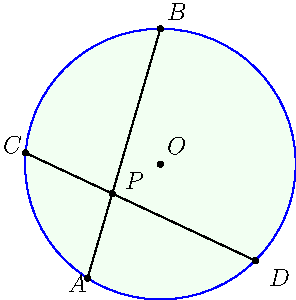
\includegraphics{pop-case2.pdf}
	\caption{Power of a Point}
\end{figure}


\section{Radical Axis}
What is radical axis? Radical axis is a set of points which have equal power with respect to two circles. It is a straight line and easy to prove using cartesian co-ordinates.

It is easy to draw the radical axis of two intersecting circles, but if thye are not intersecting then we have to draw another circelwhich intersect the two circles, then by the radical center, we can find hte radical axis.


Suppose that we have given three distinct circle, where pairwise radical axes are not parallel then they must concur. This (the point of concurrency) is called \vocab{Radical Center} of three circles.


Now we are going to see some example of problem solving using power of a point.

\begin{example}
Let $ABC$ be an acute triangle. Let the line through $B$ perpendicular to $AC$ meet the
circle with diameter $AC$ at points $P$ and $Q$, and let the line through $C$ perpendicular
to $AB$ meet the circle with diameter $AB$ at points $R$ and $S$. Prove that $P, Q, R, S$ are
concyclic.
\end{example}

\begin{figure}[ht]
\centering
	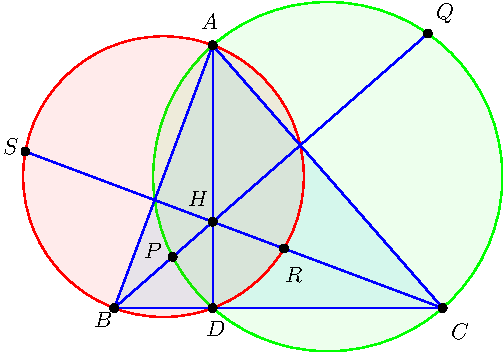
\includegraphics{radax-prob2.pdf}%[scale=0.5]{pop-prob1.png}
	\caption{Soving a problem using PoP}
\end{figure}


\begin{soln}
Let $D$ be the foot of the perpendicular from $A$ to $BC$ andlet $H$ be the orthocenter of $ABC$. Since, $\angle ADB =90\dg$, the circle with diameter $AB$ passes through $D$, so $HS \cdot HR =
HA \cdot HD$ by power of a point. 

Similarly the circle with diameter $AC$ passes through $D$
as well, so $HP \cdot HQ = HA \cdot HD$ as well. Hence $HP \cdot HQ = HR \cdot HS$, and therefore by
the converse of power of a point, $P, Q, R, S$ are concyclic.
\end{soln}

\section{PoP for showing Concurrency}

\begin{example}[IMO 1995]
Let $A, B, C$, and $D$ be four distinct points on a line, in that order. The
circles with diameters $AC$ and $BD$ intersect at $X$ and $Y$ . The line $XY$ meets $BC$ at $Z$.
Let $P$ be a point on the line $XY$ other than $Z$. The line $CP$ intersects the circle with
diameter $AC$ at $C$ and $M$ , and the line $BP$ intersects the circle with diameter $BD$ at $B$
and $N$ . Prove that the lines $AM , DN$ , and $XY$ are concurrent.
\end{example}

\begin{figure}[ht]
\centering
	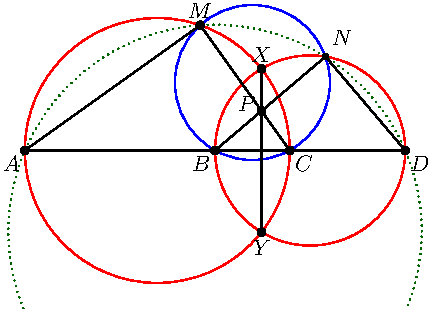
\includegraphics{pop-concur.pdf}%[scale=0.5]{pop-concur.png}
	\caption{PoP for showing Concurrency}
\end{figure}

\begin{soln}
By power of a point we have \(PM \cdot PC= PX\cdot PY =PN \cdot PB \). So, \(B,C,M,N\) are concyclic. Note that $\angle AMC = \angle BND = 90\dg$ since they are subtended by diameters $AC$ and $BD$, respectively. Hence $\angle MND = 90\dg + \angle MNb = 90\dg + \angle MCA = 180\dg -\angle MAD $.

Therefore, $A,D,N,M$ are concyclic. Since $AM,DN,XY$ are thethree radical axes for the circumcircles of $AMXC,BXND$ and $AMND$, they concur at the radical center.

\end{soln}

\section{PoP for showing Collinearity}

\begin{example}
Let $ABC$ be a triangle and let $D$ and $E$ be points on the sides $AB$ and $AC$, respectively,
such that $DE$ is parallel to $BC$. Let $P$ be any point interior to triangle $ADE$, and let $F$
and $G$ be the intersections of $DE$ with the lines $BP$ and $CP$ , respectively. Let $Q$ be the
second intersection point of the circumcircles of triangles $PDG$ and $PFE$. Prove that the
points $A, P$, and $Q$ are collinear.
\end{example}

\begin{figure}[ht]
\centering
	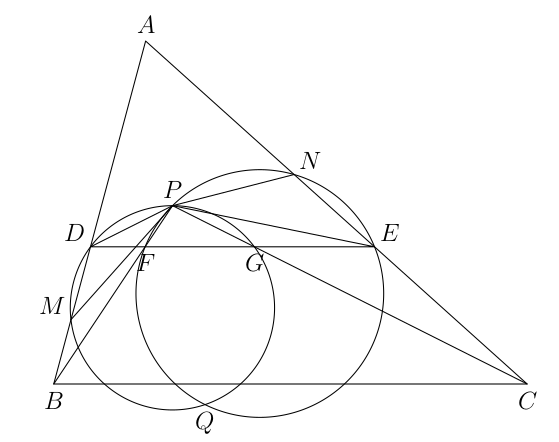
\includegraphics[scale=0.3]{pop-collinear.png}
	\caption{PoP for showing Collinearity}
\end{figure}

\begin{soln}
Let the circumcircle of $DPG$ meet line $AB$ again at $M$ , and let the circumcircle of $EPF$
meet line $AC$ again at $N$ . Assume the configuration where $M$ and $N$ lie on sides $AB$
and $AC$ respectively (the arguments for the other cases are similar). We have $\angle  ABC =
\angle  ADG = 180 \dg - \angle  BDG = 180 \dg - \angle M P C,$ so $BMPC$ is cyclic. Similarly, $BPNC$ is
cyclic as well. So $BCNPM$ is cyclic. Hence $\angle AN M = \angle ABC = \angle ADE,$ so $M, N, D, E$
are concyclic. By power of a point, $AD \cdot AM = AE \cdot AD$. Therefore, $A$ has equal power
with respect to the circumcircles of $DPG$ and the $EPF$ , and thus $A$ lies on line $PQ$, the radical axis.

\end{soln}

Here I am going to include some problems which can be solved using Power of a Point.
\begin{problem}[IMO 2000/1]
Two circles $G_1$ and $G_2$ intersect at two points $M$ and $N$ . Let
$AB$ be the line tangent to these circles at $A$ and $B$, respectively, so that $M$ lies closer to $AB$
than $N$ . Let $CD$ be the line parallel to $AB$ and passing through the point $M$, with $C$ on $G_1$
and $D$ on $_2$ . Lines $AC$ and $BD$ meet at $E$; lines $AN$ and $CD$ meet at $P$ ; lines $BN$ and
$CD$ meet at $Q$. Show that $EP = EQ$.
	\begin{hint}
		\addhint{}
		\addhint{}	
	\end{hint}
\end{problem}

\begin{problem}[USAMO 1997/2]
Let $ABC$ be a triangle. Take points $D, E, F$ on the
perpendicular bisectors of $BC, CA, AB$ respectively. Show that the lines through $A, B, C$
perpendicular to $EF , F D, DE$ respectively are concurrent.
	\begin{hint}
		\addhint{}
		\addhint{}	
	\end{hint}
\end{problem}

\begin{problem}[USAJMO 2012/1]
Given a triangle $ABC$, let $P$ and $Q$ be points on segments
$AB$ and $AC$, respectively, such that $AP = AQ$. Let $S$ and $R$ be distinct points on segment
$BC$ such that $S$ lies between $B$ and $R$, $\angle BPS = \angle PRS$, and $\angle CQR = \angle QSR$. Prove
that $P , Q, R, S$ are concyclic.
	\begin{hint}
		\addhint{}
		\addhint{}	
	\end{hint}
\end{problem}
%\section{}

%\section{}

%\section{}


\chapter{Polynomials}% by Mursalin Habib}

\begin{linkb}
   \begin{itemize}
        \item \href{https://www.youtube.com/watch?v=w52vpcuTAwo}{Polynomial (Mursalin)}
        \item \href{https://drive.google.com/file/d/1SoVQm_j-osYbXPg7ZHeS3hQdGCw9m0Yo/view}{Polynomials Pset}
   \end{itemize}
\end{linkb}


What is a polynomial? Well, an example of a polynomial is given below:
\[x^2-5x+6.\]
Generally a polynomial is a form of:
\[a_nx^n + a_{n-1}x^{n-1} + a_{n-2}x^{n-2}+ \ldots + a_2x^2 + a_1x + a_0 .\]
where $a_n\neq 0$. Also assume that $a_n, a_{n-1}, \ldots$ are generally real numbers. 
%otherwise  
Here comes some definitions:
\begin{definition}[Coefficient]
$a_n,a_{n-1}, \ldots$ are called coefficients.
\end{definition}
\begin{definition}[Leading Coefficient]
$a_n$ is called the leading coefficient.
\end{definition}
\begin{definition}[Degree of a polynomial]
Maximum power $n$ is called the degree of a polynomial.
\end{definition}
\begin{definition}[Monic Polynomial]
A polynomial with leading coefficient $1$ is called a monic polynomial.
\end{definition}
\begin{definition}[Root of polynomial]
For a polynomial, $P(x)=a_nx^n + a_{n-1}x^{n-1} + a_{n-2}x^{n-2}+ \ldots + a_2x^2 + a_1x + a_0$. Roots of polynomial are the set of variables for which $P(x)=0$.
\end{definition}
\begin{theorem}[Fundamental theorem of Algebra]
For any n-degree polynomial, there are at most n distinct roots.
\end{theorem}
Here we are introduced with some techniques to solve polynomial problems:
\section{Exploiting Symmetry}
\begin{example}
Find all real $x$ that satisfy the equation
\[(x-1)(x^2+1)(x^3+1)=30x^3.\]
\end{example}
Here do some algebra to get:
\[x^6 + x^5 + x^4 -28x^3 +x^2 +x+1=0.\]
It is a polynomial of degree $6$ which is messy.
But you can see that here is a symmetry left to the term $-28x^3$ with the right part of the equation. 
Also observe that, if $x$ is a root then $\frac{1}{x}$ is also a root. 
So, we are going to divide the equation by $x^3$ and we get:
\[x^3+x^2 +x -28 +\frac{1}{x}+\frac{1}{x^2}+\frac{1}{x^3}=1.\]
Here we pair up $x^3$ with $\frac{1}{x^3}$ and so on. We get the following: 
\[\left(x^3+\frac{1}{x^3}\right)+\left(x^2+\frac{1}{x^2}\right)+\left(x+\frac{1}{x}\right)-28=0.\]
Now we assume $x+\frac{1}{x}=y$ and you see that, $x^3+\frac{1}{x^3}=y^3-3y, x^2+\frac{1}{x^2} =y^2-2y, x+\frac{1}{x}=y$ and we proceed by following:
\begin{align*}
\left(x^3+\frac{1}{x^3}\right)+\left(x^2+\frac{1}{x^2}\right)+\left(x+\frac{1}{x}\right)-28&=0\\
y^3 -3y +y^2 -2y +y-28 &=0\\
y^3 +y^2 -2y-30 &=0
\end{align*}
But it is a polynomial with degree $3$, which is also not so easy to solve. But we have a theorem for this: Rational Root Theorem.
%\begin{theorem}[Rational Root Theorem]
%A polynomial $P(x)$ has a rational root $\frac{p}{q}$ if and only if $p|a_0$ and $q|a_n$. 
%\end{theorem} 
if we can find a root of our polynomial then it comes easy to solve a quadratic eqaution.

After playing with numbers, you can find a root $3$ which works!
Then we have, \[(y-3)(\ldots)=y^3+y^2-2y-30.\]
Now, you can solve the problem  and the rest is a good exercise so left as an exercise.

Here we see another problem:
\begin{example}
Find all real solution to the eqaution,
\[x^4 +(x-2)^4=34.\]
\end{example}
It is a $4$ degree polynomial, so we have to think wisely.
An idea coomes that, we can rewrite the equation by folling, \[(y+1)^4+(y-1)^4=34\]
where, $x=y+1$ and so $x-2=y-1$ After doing 
some algebra we get a polynomial where all 
the degrees of $y$ is even, and assume $y^2=z$ 
then the polynomial is a quadratic and do some algebra.

\section{Polynomial Division}
You probably know that for a number $a$ we can find $q$ such that $q|a$ and we can write $a$ as follows:
\[a=bq+r\] where $0\le r<b$.

Similarly for a polynomial $a(x)$ we can find $b(x), q(x)$ and $r(x)$ such that,
\[a(x)=b(x)q(x) +r(x).\]
Here note that if $b(x)$ has degree $2$ then $r(x)$ is linear.

By using these facts we can solve a problem now:
\begin{example}
Find the remainder when the polynomial $x^{81}+x^{49}+x^{25}+x^9 +x$ is divided by the polynomial $x^3-x$.
\end{example}
 Here observe that we can write the polynomial by $Q(x)(x^3-x) +r(x)$ and also observe that $r(x)$ has degree $2$.
 So,
 \[x^{81}+x^{49}+x^{25}+x^9 +x=Q(x)(x^3-x) +ax^2+bx+c.\]
 Now we factor, \[x^3-x=x(x+1)(x-1).\]
 Now, pluging $x=0, x=1, x=-1$ in the above equation we get, \[a=0, b=5, c=0\]
 so, the remainder is $5x$.


 Always remember to write a polynomial $a(x)$ by $b(x)q(x)+r(x)$.

 Also remember the vieta's formulas. It  Assume that the polynomial 
 \[a_nx^n + a_{n-1}x^{n-1} + a_{n-2}x^{n-2}+ \ldots + a_2x^2 + a_1x + a_0 .\]
 has roots $r_1, r_2, r_3, \ldots , r_n$
  we have 
  \[ r_1+r_2+r_3+\ldots + r_n =-\frac{a_{n-1}}{a_n}\]
 and, \[r_1r_2 +r_2r_3 +\ldots +r_{n-1}r_n=\frac{a_{n-2}}{a_n}\]
 and similarly analogous...

 Here are going to solve a problem using the above proposition.

\begin{example}
Given that, $a+b+c>0$, $ab+bc+ca>0$ and $abc>0$. Prove that, $a,b,c>0$.
\end{example}
Here we will use method of contradiction!

%Assume that, 
We are going to construct a polynomial:
\[P(x)=x^3 -(a+b+c)x^2+(ab+bc+ca)x-abc\]
which has roots $a,b,c$.

And assume that $a$ is negative. But then $P(a)$ is negative which is supposed to be zero(as $a$ is a root of $P(x)$). Which is a contradiction!


\begin{example}
Let $n$ be a positive integer and for $1\le k \le n$ let $s_k$ be the sum of the products of the numbers $1, 1/2, 1/3,\ldots, 1/n$ taken $k$ at a time.
For example,
\[s_2 = 1\cdot \half + 1 \cdot \frac{1}{3} + \ldots \frac{1}{n-1}\cdot \frac{1}{n}\]
Find $s_1 +s_2 +\ldots + s_n$.
\end{example}
It is left as an exercise for the interested readers.
%\ldots

%left as an exercise
\begin{theorem}[Identity Theorem]
Two polynomials $f(x), g(x)$ have degree less than $n$. If they intersect at $n+1$ points ($x_1, x_2, \ldots x_{n+1}$) so, $f(x_1)=g(x_1), f(x_2)=g(x_2), \ldots $.

Then two polynomials are the same i.e. $f(x)=g(x)$.
\end{theorem}
Here let $P(x)=f(x)-g(x)$, it results that, $P(x)$ has $n+1$ roots which is not possible unless $P(x)$ is identically zero. (as $P(x)$ has degree at most $n$.)

Here, we solve a problem using the above result.
\begin{example}
If $f(x)$ is a monic quartic polynomial such that $f(-1)=-1, f(2)=-4, f(-3)=-9$ and $f(4)=-16$. Find $f(1)$.
\end{example}

$f(-1)=-1, f(2)=-4, f(-3)=-9$ and $f(4)=-16$
So, $f(x)=-x^2$ which is not a monic polynomial.

We asssume $f(x)=x^4 + bx^3 + cx^2 +dx +e$ as it is monic and quartic.

Then, consider the polynomial $f(x)+x^2=P(x)$ which is a 4 degree polynomial which has roots $-1, 2, -3, 4$.

At these points $P(x)$ is zero, and as it is a quartic so we have, \[P(x)=c(x+1)(x-2)(x+3)(x-4)\]
where $c$ is obviously zero as $f(x)$ is a monic.

\begin{example}
If $P(x)$ denotes a polynomial of degree $n$ such that \[P(k)=\frac{k}{k+1}\]
for $k=0,1,2,\ldots, n$. Determine $P(n+1).$
\end{example}
Here conisder a polynomial \[(x+1)P(x)-x=f(x)\]
by the above argument, we get, \[f(x)=cx(x-1)(x-2)(x-3)\cdots (x-n)\]
Plugging $x=-1$ we get, $1=c(-1)^{n+1}(n+1)!$
so, \[c=\frac{1}{(-1)^{n+1}(n+1)!}\]
The rest is a good exercise.

\section{Polynomial Interpolation}%, Polynomial Functional Equation}
Suppose you are given that $f(1)=7, f(2)=4, f(10)=-5$ and you are told to find the function. This process is called Polynomial Interpolation. The above problem asks you to find the polynomial which graph goes through the points $(1,7), (2,4), (10,-5)$.

\begin{example}
What is the next term of the sequence $2,5,11,23,\ldots $?
\end{example}
The answer is what you want!

We write $n$ term as $a_n$ and let \[a_n=(A_1 \times 2) + (A_2\times 5) + (A_3 \times 11) + (A_4 \times 23) + (A_5 \times 42)\]
Take $A_1, _2, A_3, A_4, A_5$ such that if we plug $n=1$ then we get $A_1=1$ and $A_2=A_3=A_4=A_5=0$. Similarly for $n=2,3,4,5$.
Magically take \[A_1=\frac{(n-2)(n-3)(n-4)(n-5)}{(1-2)(1-3)(1-4)(1-5)}\]

and analogous for $A_2, A_3 ,\ldots$

\begin{example}
$f$ be a function such that $f(1)=7, f(2)=4, f(10)=-5$
\end{example} 
From the above example it is easy. 
So,
\[f(x)=\frac{(x-2)(x-10)}{(1-2)(1-10)} \times 7 + \frac{(x-1)(x-10)}{(2-1)(2-10)} \times 4 + \frac{(x-1)(x-2)}{(10-1)(10-2)} \times (-5)\]
It is known as Lagrange Interpolation.
It is useful in finding an algebraic form of a sequence.

\begin{example}
\[f(x)=\frac{(x-b)(x-c)}{(a-b)(a-c)} + \frac{(x-a)(x-c)}{(b-a)(b-c)} + \frac{(x-a)(x-b)}{(c-a)(c-b)}\]
and $a\neq b \neq c$.
$\deg(f)\le 2$.
%What is the degree of $f$?
\end{example}

We get, $f(a)=f(b)=f(c)=1$. So, it is not possible to have degree 2. As it has same value at three points.

Consider $f(x)-1=p(x)$, and $p(a), p(b), p(c)$ is zero. So, $p(x)$ is identically zero and $f(x)=1$.

\begin{example}
Let $a,b,c,d$ be distinct real numbers. Show that \[\frac{a^4}{(a-b)(a-c)(a-d)}+\frac{b^4}{(b-a)(b-c)(b-d)}+\frac{c^4}{(c-a)(c-b)(c-d)}+\ldots=a+b+c+d.\]
%%%%%%%\[\frac{a^4}{(a-b)(a-c)(a-d)}+\frac{b^4}{(b-a)(b-c)(b-d)}+\frac{c^4}{(c-a)(c-b)(c-d)}+\frac{d^4}{(d-a)(d-b)(d-c)}=a+b+c+d.\]
\end{example}
\[P(x)=\frac{a^4(x-b)(x-c)(x-d)}{(a-b)(a-c)(a-d)}+\frac{b^4(x-a)(x-c)(x-d)}{(b-a)(b-c)(b-d)}+\frac{c^4(x-a)(x-b)(x-d)}{(c-a)(c-b)(c-d)}+\ldots\]

%%%%\[P(x)=\frac{a^4(x-b)(x-c)(x-d)}{(a-b)(a-c)(a-d)}+\frac{b^4(x-a)(x-c)(x-d)}{(b-a)(b-c)(b-d)}+\frac{c^4(x-a)(x-b)(x-d)}{(c-a)(c-b)(c-d)}+\frac{d^4(x-a)(x-b)(x-c)}{(d-a)(d-b)(d-c)}\]

The coefficient of $x^3$ in $P(x)$ 

\[f(x)=x^4-P(x)=(x-a)(x-b)(x-c)(x-d).\]

\section{Practice Problems}
\begin{problem}
Find all real x that satisfy the equation
\[ (x+1)(x^2+1)(x^3+1)= 30x^3 \]
\begin{hint}
\addhint{}
\addhint{}
\end{hint}
\end{problem}
\begin{problem}
Find all real solutions to $ x^4 +(x-2)^4 = 34$.
\begin{hint}
\addhint{}
\addhint{}
\end{hint}
\end{problem}
\begin{problem}
Find the reminder when $x^81 + x^49 +x^25 + x^9 +x $ is divided by the polynomial $x^3-x$
\begin{hint}
\addhint{}
\addhint{}
\end{hint}
\end{problem}
\begin{problem}
Let $P(x) = x^4 + ax^3 + bx^2 + cx + d$ where $a$, $b$, $c$ and $d$ are constants. If $P(1) = 10$, $P(2) = 20$ and $P(3)= 30$. Compute,
\[\frac{P(12)+ P(-8)}{10} \]
\begin{hint}
\addhint{}
\addhint{}
\end{hint}
\end{problem}
\begin{problem}
Find $x^2+y^2 $ if $x$ and $y$ are positive integers such that,
\[xy + x+ y = 71 \text{ and } x^2y +xy^2 =880\]
\begin{hint}
\addhint{}
\addhint{}
\end{hint}
\end{problem}
\begin{problem}
Let $n$ be a positive integer, for $1\le k \le n$, let $s_k$ be the sum of the products of the numbers $1, 1/2,1/3,  \ldots ,1/n$, taken $k $ at a time. For example, 
\[ s_2 = 1.\frac{1}{2} + 1.\frac{1}{3}+ \ldots +\frac{1}{n-1}.\frac{1}{n} \] 
Find $s_1 +\ldots s_n$.
\begin{hint}
\addhint{}
\addhint{}
\end{hint}
\end{problem}
\begin{problem}
Let $a$, $b$ and $c$ be real numbers such that $a+b+c>0$, $ab+bc+ca>0$ and $abc>0$. Prove that $a,b$ and $c$ are all positive
\begin{hint}
\addhint{}
\addhint{}
\end{hint}
\end{problem}
\begin{problem}
Let $r,s$ and $ t $ be the three roots of the equation
\[ 8x^3 + 1001x +2008=0\]
Find $(r+s)^3 + (s+t)^3 + (t+r)^3$.
\begin{hint}
\addhint{}
\addhint{}
\end{hint}
\end{problem}
\begin{problem}
If $f(x)$ is a monic polynomial such that $f(-1)=-1$, $f(2)=-4$, $f(-3)= -9$ and $f(4)=-16$. Find $f(1)$.
\begin{hint}
\addhint{}
\addhint{}
\end{hint}
\end{problem}
\begin{problem}
If $P(x)$ denotes a polynomia of degree $n$ such that \[P(k) = \frac{k}{k+1}\]
for $k= 0,1,\ldots ,n$, determine $P(n+1)$.
\begin{hint}
\addhint{}
\addhint{}
\end{hint}
\end{problem}
\begin{problem}
Let $a_1, a_2, a_3, \ldots, a_{10} $ be real numbers such that, 
\[\frac{a_1}{1}+ \frac{a_2}{2} +\ldots + \frac{a_{10}}{10} =1 \]
\[\frac{a_1}{2}+ \frac{a_2}{3} +\ldots + \frac{a_{10}}{11} =0 \]
\[\frac{a_1}{3}+ \frac{a_2}{4} +\ldots + \frac{a_{10}}{12} =0 \]
\[\ldots\]
\[\frac{a_1}{10}+ \frac{a_2}{11} +\ldots + \frac{a_{10}}{19} =0 \]
 Determine $a_1+a_2+ \ldots a_10$.

\begin{hint}
\addhint{}
\addhint{}
\end{hint}
\end{problem}
\begin{problem}
Let $a,b,c$ and $d$ be distinct real numbers. Show that 
\[\frac{a^4}{(a-b)(a-c)(a-d)}+\frac{b^4}{(b-a)(b-c)(b-d)}+\frac{c^4}{(c-a)(c-b)(c-d)}+\ldots=a+b+c+d.\]
\begin{hint}
\addhint{}
\addhint{}
\end{hint}
\end{problem}
\begin{problem}
A polynomial of degree $3n$ takes the value $0$ at $2,5,8,\ldots,3n-1$. The value $1$ at $1,4,7,\ldots, 3n-2$ and the value $2$ at $0,3, \ldots, 2n$ and its value at $3n+1$ is $730$. Find $n$.
\begin{hint}
\addhint{}
\addhint{}
\end{hint}
\end{problem}
\begin{problem}
Find all polynomials $P(x)$ with real coefficients that satisfy
\[(x-1)P(x)-xP(x-1)= x^2-x-1\]
for all real number $x$.
\begin{hint}
\addhint{}
\addhint{}
\end{hint}
\end{problem}
\begin{problem}
Suppose that $P(x)$ is a polynomial of odd degree satisfying 
\[P(x^2-1)=(P(x))^2 -1\]
for all $x$. Prove that $P(x)= x$ for all $x$.
\begin{hint}
\addhint{}
\addhint{}
\end{hint}
\end{problem}

\chapter{Transformation}% by Mugdho Tanjim Shorif}

\begin{linkb}
   \begin{itemize}
        \item  \href{https://www.youtube.com/watch?v=yohxAxqnCt8}{Video 1}, \href{https://www.youtube.com/watch?v=7tAmJ8cvmYM}{Video 2}
        \item \href{https://drive.google.com/file/d/1_XBfSBLO3NSWAKw9_mkhYPIWgkRfwm2Z/view}{(Boby Poon) } + \href{https://drive.google.com/file/d/11kMt5af6pfZDoaV932MsEf6Sx0vvznsk/view}{The Real Big Picture}
   \end{itemize}
\end{linkb}


There are generally  5 kind of Transformation, namely:
\begin{itemize}
	\item Translation
	\item Rotation
	\item Reflection
	\item Homothety
	\item Spiral Similarity		
\end{itemize}

\section{Translation}
This is the most common  and easy of the transformations, you can translate a point along with a line. Let the point is $P$ and the line is $AB$, then if you translate $P$ wrt $AB$, we write this as $T(AB)$ and here $P$ maps to a point $Q$ such that $AB \parallel PQ, $ and $AB=PQ$.

\begin{figure}[ht]
\centering
	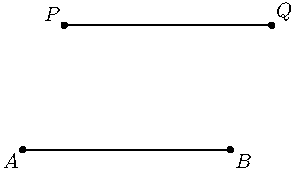
\includegraphics{translate1.pdf}
	\caption{Translation along with $AB$ maps $P$ to $Q$.}
\end{figure}

Here we are going to solve some problem.
\begin{example}
In the figure below, what is the minimal distance from $A$ to $B$ with a bridge that can be made in anywhere over the river perpendicular to the parallel lines.
\end{example}

\begin{figure}[ht]
\centering
		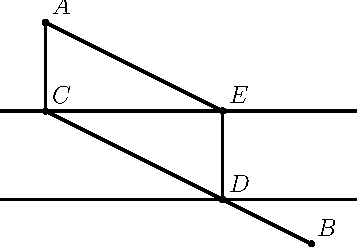
\includegraphics{translate2.pdf}
	\caption{Find shortest path from $A$ to $B$.}
\end{figure}

\begin{problem}
Similarly above find the shrtest distance from $A$ to $B$ with more that one river between them.
\end{problem}

\begin{example}
Let $ABCDEF$ be a hexagon such that, $AB\parallel DE, BC \parallel EF, CD \parallel FA$ and $AF-CD=DE-AB = BC -EF >0$. Prove that the hexagon is equiangular that is all the angles of the hexagon is equal  to $120\dg$.
\end{example}

\begin{figure}[ht]
\centering
	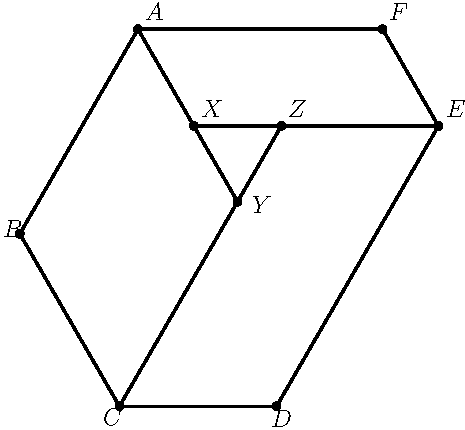
\includegraphics{translate3.pdf}
	\caption{Finding an equilateral triangle}
\end{figure}

Here the opposite sides configuration is very disgusting to handle. So we want such a translation which makes the subtraction of th opposite sides to the side of an equilateral triangle. We are going to translate $E$ along with $AF$ to map $E$ to $X$, similarly define $Y,Z$. Now observe that $XYZ$ is an equilateral triangle. Now it is easy to conclude.


\begin{example}
In quadrilateral $ABCD$, let $M,N$ be the midpoints of $AB$ and $CD$ respectively. Given that, $@MN=AD+BC$. Prove that, $AD\parallel BC$. 
\end{example}

%--------
\section{Rotation}
Rotation deals with a center point and an angle. Let a point be $P$ and another center point $O$. You may rotate $P$ wrt $O$ with angle $50\dg$ which means you draw an arc with center $O$ and goes from $P$ to $Q$.
And $\angle POQ =50\dg$.
It is defined by \[R(O,\alpha)\]
\begin{example}
Let, $ABCD$ be a square and $P$ be a point inside the square such that, $PA=1, PB=2, PC=3$. Find $\angle APB$.
\end{example}

Here we are going to rotate the points $A,C,P$ with center $B$ and angle of $90\dg$. Which means $A\mapsto C, P\mapsto P'$. Now note that as $\angle PBP'=90\dg$ and $PB=BP'$, we have, $\angle BPP'=45\dg=BP'P$. By Pythagoras, $PP'=2\sqrt 2$. As $AP =CP'=1$,  by the converse of Pythagoras we have, $\angle PP'C =90\dg$. So $\angle APB = \angle CP'B =90\dg$.

\begin{example}
Let $ABC$ be an equilateral triangle and a point inside the triangle $P$ such that $PA=5, PB=4, PC=3$. Find the area of the triangle.
\end{example}
\begin{figure}[ht]
\centering
		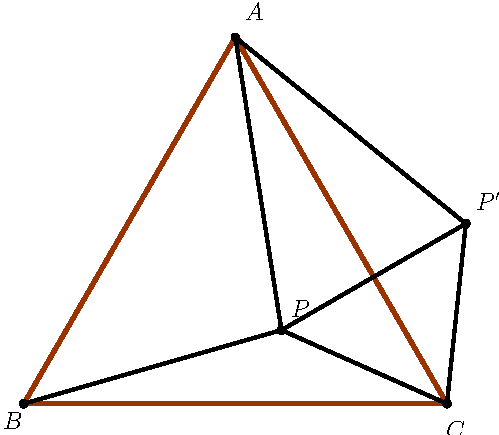
\includegraphics{rotate1.pdf}
	\caption{Rotate the point $P$}
\end{figure}
Consider a rotation with center $C$ and angle $60\dg$, $P\mapsto P', B\mapsto A$ and see that, \[CP'=CP\]
\[CA=CB\]
\[\angle P'CA = \angle PCB\]
Here you see that, \[AP'=BP=4\]
\[PP'=3\]
and $APP'$ is a right angular triangle with $\angle AP'P=90\dg$.
So, \[ \angle AP'C=150\dg=\angle BPC \]
By cosine law we are done!


\begin{example}
Let $ABCD$ be a square and $W,X,Y,Z$ be four points on $AB,BC,CD,DA$ respectively such that $BW+BX+DY+DZ=2BC$. Prove that, $WY\perp ZX$. 
\end{example}
Here rotate the diagram with center $B$ and
 angle $90\dg$. We denote the rotation of $A$
  with $A'$ and analogous...


AND we are giong to show that $WY \parallel Z'X'$
\begin{figure}[ht]
\centering
		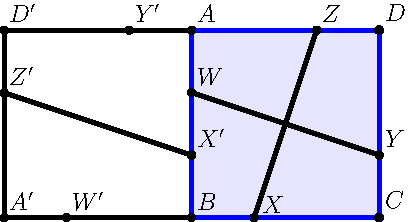
\includegraphics{rotate2.pdf}
	\caption{Perpendicularity to Parallelism!}
\end{figure}
Here we let $AB=BC=CD=DA=a$.
And doing some calculation:
\begin{align*}
BW+BX+DY+DZ &=2BC=2a\\
BW'+BX+D'Y'+DZ &=2a\\
BW'+BX+(a-AY')+(a-AZ) &=2a\\
BW'+BX &= AY'+AZ\\
XW'&=Y'Z
\end{align*}
Now it is easy to see that $XZY'W'$ is a parallelogram. And that's why $ZX\parallel W'Y'$.
%------------
\section{Reflection}

\begin{example}
Let $ABCD$ be a quadrilateral such that, $AB=BC=CD$ and $AC \neq BD$ but $AE=DE$ where $E$ is the intersection of the diagonals. Find $\angle BAD + \angle ADC$.
\end{example}

\begin{figure}
\centering
	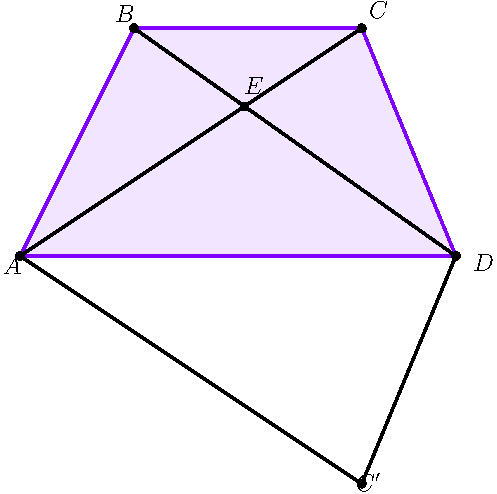
\includegraphics{reflection1.pdf}
 	\caption{A reflection problem}
 \end{figure}
Here we are goingt to reflect $C$ with respect to $AD$ and we get that $BD\parallel AC'$ and $C'D=AB$. SO $ABDC'$ is either a parallelogram or trapezoid. 

But there is a contradiction that if it is a paralleogram then $AC'=AC=BD$ which is absurd.

So it is an isosceles trapezoid which is obviously cyclic.
Here we denote $\angle BAC=\beta=\angle BCA$, $\angle CAD =\angle DAC'=\angle BDA=\alpha$, $\angle DBC=\gamma$.

So we get $\angle ADC'=\alpha +\gamma $
Using cyclic quads, we get $4\alpha=120\dg$. (Yes, there is some angle chasing which is a good exercise and left to the reader.)

Here is a problem you can try:
\begin{problem}
A circle with center $O$ passes through vertices $A$ and $C$ of $\triangle ABC$ and cuts sides $AB,BC,CA$ at $K$ and $N$ respectively. The circumcircles of $ABC$ and $KBN$ intersect at $B$ and $M$. Prove that $\angle OMB=90\dg$.
\end{problem}

\section{Homothety}
Homothety (also known as dilation) is a 
transformation consisting of two variables- 
a center $O$ and a real number $k$ such that
$O$ sends a point $A$ to $A'$.
Homothety is denoted by-
\[ H(O, k)\]
Remember that $k$ can be negative

We have, \[ \frac{OA'}{OA}=k.\]

\begin{enumerate}
	\item After homothety $AB$ and $A'B'$ are parallel.
	\item Triangles are similar after homothety.
	%\item
\end{enumerate}
See the diagram. Here $O$ sends $A, B, C$ to $h(A), h(B), h(C)$ respectively.

\begin{figure}[ht]
\centering
	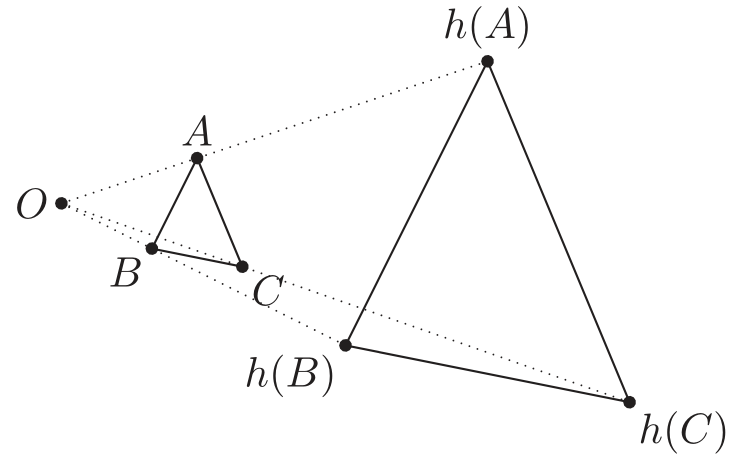
\includegraphics[scale=0.3]{homothety.png}
	\caption{$\triangle ABC$ and $\triangle  h(A), h(B), h(C)$ are homothetic similar}
\end{figure}
As said before $k$ can be negative. See the diagram-

\begin{figure}[ht]
\centering
	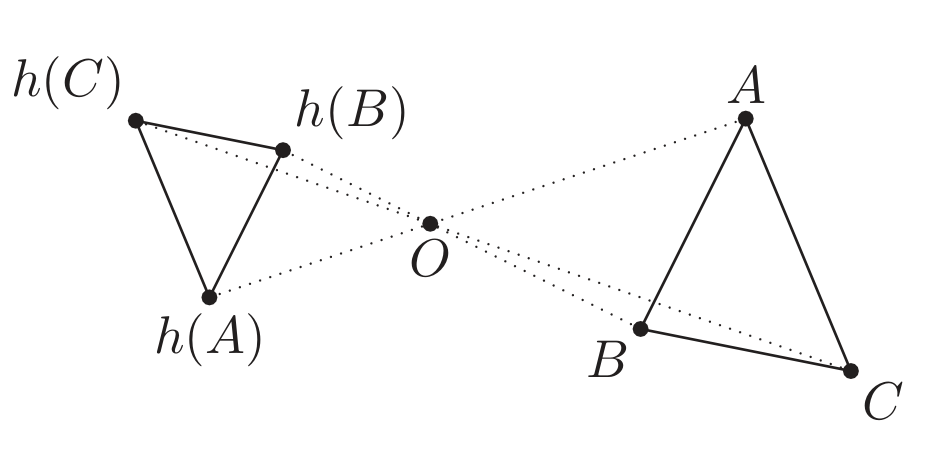
\includegraphics[scale=0.3]{neg-homothety.png}
	\caption{A negative homothety}
\end{figure}
Also remember that homothetic center can be a point at infinity. Where $AB=A'B'$ and the scale factor of the homothety is not equal to $-1$.



\begin{example}
Two circles $C_1, C_2$ are such that $C_2$ is internally tangent  to $C_1$ at $P$. A chord $AB$ of $C_1$ touches $C_2$ at $E$. Prove that ray $PE$ bisects the arc $AB$ which doesn't contains $P$.
\end{example}

We are going to use homothety here. Look
 that $P$ is the homothetic center of two 
 circles that sends $C_2$ to $C_1$.
Let $O_1, O_2$ vare the centers of $C_1, C_2$ respectively, see that $P,O_1,O_2$ are collinear.
Also $P,E,F$ (where $F$ is the intersection point of $PE$ with $C_1$) are collinear. Consequently $PO_2E$ and $PO_1F$ are homothetic. Here note that $\angle O_2EA=90\dg$ similarly $F$ is the tangent point of a line parallel to $BA$ whch is tangent to $C_1$. 

Here we see a proof of the nine point circle.
\begin{figure}[H]
\centering
	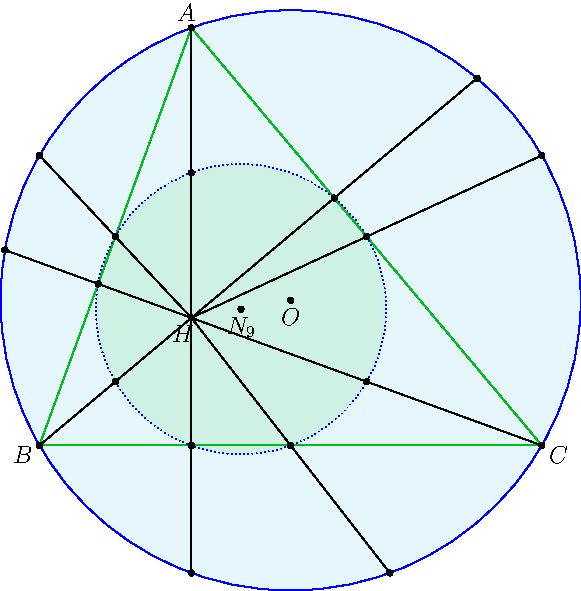
\includegraphics{npc-homo.pdf}%[scale=0.3]{npc.png}
	\caption{Nine Point Circle Homothetic to $(ABC)$ with center $H$.}
\end{figure}
You probably know the fact that the reflection of the orthocenter on the line $BC$ and with respect to the midpoint of $BC$ lies on the circumcircle of $ABC$.
Similarly, define analogous points.
Here you get nine points on the circumcircle of $ABC$. Consider a homothety with center $H$ and scale factor $\half$. So we get nine points still concyclic. Done!

\begin{problem}\label{prob:homo}
Let the incircle of triangle $ABC$ touches $BC$ at $D$. $T$ is the antipode of $D$ with respect to the incircle. Let ray $AT$ meets $BC$ at $P$. Prove that $BD=CP.$
\end{problem}


\begin{figure}[ht]
\centering
	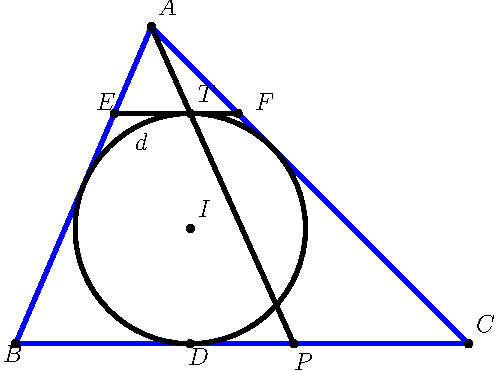
\includegraphics{homo-prob.pdf}
	\caption{\autoref{prob:homo} for exercise}
\end{figure}

\section{Spiral Similarity}
Spiral similarity isa special kind of similarity consisiting of a rotation and a dilation(homothety). It is denoted by \[S (O,\alpha ,k)\] where $O$ is the center of the spiral similarity.
%or denoted by S 

\begin{example}
$P$ is an internal point in the plane of a triangle $ABC$ such that $\angle APC=\angle BPC=\angle APB=120\dg$ and $\angle BAC =60\dg$. Let, $D,E$ be the midpoints of the segments $AC,AB$ respectively. Show that $AEPD$ cyclic.
\end{example}
\begin{figure}[ht]
\centering
	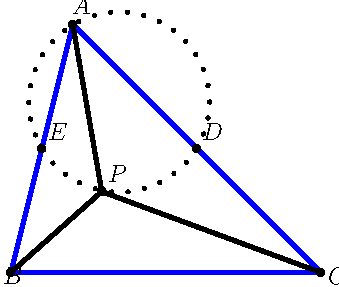
\includegraphics{spiral1.pdf}
	\caption{A spiral similarity problem}
\end{figure}
Here see that $\triangle APB$ and $\triangle CPA$ aer similar.
So we can take a spiral similarity that takes $APB$ to $CPA$ with center $P$ and angle $120\dg$.
\[S(P,120\dg,\frac{PC}{PA})\]
\[A\mapsto C\]
\[B\mapsto A\]
So we can say that \[E\mapsto D.\]
So, as our angle of rotation was $120\dg$ so $\angle EPD=120\dg=180\dg - \angle EAD.$
Done!

%And class ends here!








\chapter{Bijection}% by Ahsan Al Mahir}

\begin{linkb}
   \begin{itemize}
        \item \href{https://www.youtube.com/watch?v=Pw0VeDSC_go}{Bijection(Lazim)} 
        \item \href{https://drive.google.com/file/d/1y4aWf4oQsDQvFtwnSwT4JiFHZ_diWT1x/view}{1} , \href{https://drive.google.com/file/d/1zFTQOX1HOWcN1KMPvYR5K2okdZTXP1n1/view}{2}
   \end{itemize}
\end{linkb}

%(This class is taught by following Yufei 
%Zhao's Bijection Note. This note is a great resource for further reading.)


Bijection means a function which is injective  and surjective at the same time. 


\section{Example Problems}
Let you are told to find the number of ways to walk from $(0,0)$ to $(5,4)$. Which is 
called grid walking. It is difficult to find 
the answer unless you find some bijection. 
You may let the right  move $R$ and up move $
U$ which means all the ways are of $RURURRRUU$
 this type. Which is in fact a binary 
 string.  Now it is easier to tackle the  
 problem. And there are $\binom{9}{4}$ ways.


Our next example is about Triangular Grid. 

\begin{example}
A triangular grid is obtained by tiling an equilateral triangle of side length
$n$ by $n^2$ equilateral triangles of side length $1$. Determine the number of parallelograms
bounded by line segments of the grid.
\end{example}
\begin{figure}[ht]
\centering
	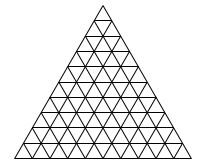
\includegraphics[scale=.5]{tri-grid.png}
	\caption{Three different oriented parallelograms}
\end{figure}
Here observe that there are 3 different types(orientation) of parallelograms.
If you can find the number of parallelograms of a single orientation, by symmetry the total number is thrice the number.

\begin{figure}[ht]
\centering
	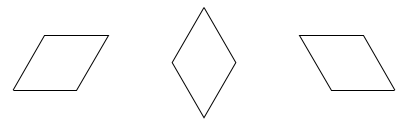
\includegraphics[scale=.5]{parallelograms.png}
	\caption{Three different oriented parallelograms}
\end{figure}
Let us
just count the paralellograms with the middle type of orientation (i.e., no horizontal
sides).

Extend the triangular grid by one extra row at the bottom. The key (and clever)
observation is that starting from any such parallelogram in the original grid, we can
extend its sides to meet the lines to meet the bottom edge of the new row in the large
triangular grid, and there would be four distinct intersection points, as shown below.
\begin{figure}[ht]
\centering
	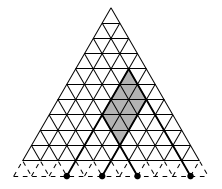
\includegraphics[scale=.5]{tri-grid-sol.png}
	\caption{An added row and the solution}
\end{figure}

Conversely, starting from any four distinct grid points in new bottom edge, we
can extend $60\dg$ lines from the first two points and $120\dg$ lines from last two points
to obtain a parallologram in the original grid. This gives us a bijection between the set
of parallelograms in the original grid with no horizontal sides with set of four distinct
points in the new bottom edge, and hence there must be $\binom{n+2}{4}$ of them. Accounting for
all three orientations, we find that the total number of parallolograms in the original
grid is $3\binom{n+2}{4}$.

(The above solution taken from Zhao's Note.)

\begin{example}
Let $n$ be a positive integer. Determine the number of lattice paths from
$(0, 0)$ to $(n, n)$ using only unit up and right steps, such that the path stays in the region $x \ge y$.
\end{example}
\begin{figure}[ht]
\centering
	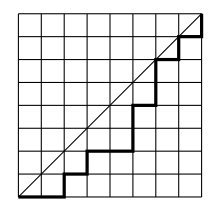
\includegraphics[scale=0.5]{grid-walk-2.png}
	\caption{The Problem}
\end{figure}


We saw previously that the total number of lattice paths from $(0, 0)$ to $(n, n)$ without the $x\ge y$ restriction is equal is $\binom{2n}{n}$. Let us count the number of paths that goes into the $x < y$ region. 
Call these paths |\textit{bad paths}.

Suppose that $P$ is a bad path. Since $P$ goes into the region $x < y$, it must hit the
line $y = x + 1$ at some point. Let $X$ be the first point on the path P that lies on the line
$y = x + 1$. Now, reflect the portion of path P up to X about the line $y = x + 1$, keeping
the latter portion of P the same. This gives us a new path $P'$.


\begin{figure}[ht]
\centering
	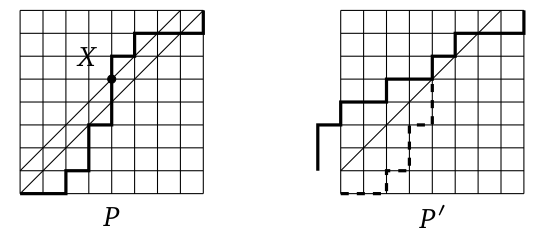
\includegraphics[scale=0.5]{grid-walk-2-sol.png}
	\caption{The Solution}
\end{figure}

We claim that this gives us a bijection between the set of bad paths to the set of
lattice paths from $(-1, 1)$ to $(n, n)$ using only up and right unit steps.

Here is the inverse construction. For any lattice path Q from $(-1, 1)$ to $(n, n)$, let $X$
be the first point on the path lying on the line $y = x + 1$, and let $Q'$ be constructed from
$Q$ by reflecting the first portion of $Q$ up to $X$ through the line $y = x + 1$ and keeping
the rest the same. Then the inverse of the bijection given above sends $Q$ to $Q'$.

To complete the proof of this claim, we need to check a number of details, which
we outline below. The reader should think about why claim is true.

\begin{itemize}
	\ii The inverse construction is well defined. That is, we can always find such a point
	$X$ , and also, the resulting $Q'$ is a always a bad path.
	\ii The two constructions are inverses of each other.
\end{itemize}
The number of bad paths is equal to the number of lattice paths from $(-1, 1)$ to
$(n, n)$ using only unit up and right steps, and there are $\binom{2n}{n+1}$ such paths.

Therefore, the total number of “good” paths, i.e., those that do not go into
the region $x < y$, is equals to 
\[\binom{2n}{n} -\binom{2n}{n+1} = \binom{2n}{n}-\frac{n}{n+1}\binom{2n}{n}=\frac{1}{n+1}\binom{2n}{n}.\]
The above number is called the Catalan Number. There are many more counting problems which are counted by Catalan Numbers.



\section{Practise Problems}
Now you can solve some problems from Yufei Zhao's Bijection Note. This note contains many problems. I am ading some of them.

\begin{problem}
Show that the $n$-th Catalan number counts the number of expressions
containing $n$ pairs of parentheses which are correctly matched. E.g., for $n = 3$,
\[((())) \ \ \ (()()) \ \ \ (())() \ \ \ ()(()) \ \ \ ()()()\]
\end{problem}

A plane tree is an object with the following structure. We start with a root vertex
(drawn at the top), and then with each node we attach a number of new vertices
(possibly none), where the order of the attached vertices matters. For instance, there
are exactly $5$ plane trees with $4$ vertices
\begin{problem}
Show that the $n$-th Catalan number counts the number of plane trees with
$n + 1$ vertices.
\end{problem}


\begin{problem}
Show that the number of ways of stacking coins in the plane so that the bottom
row consists of $n$ consecutive coins is $C_n$ .
\end{problem}



\begin{problem}
Show that the number of triangulations of a convex $(n + 2)$-gon into $n$ triangles
by $n - 1$ diagonals that do not intersect their interiors is the $n$-th Catalan number,
$C_n$.
\end{problem}

\begin{problem}
Let $n$ be a positive integer. Prove that the number of partitions of $n$ equals the
number of partitions of $2n$ with $n$ parts.
\end{problem}
%\section{}



\chapter{Prime Numbers}% by DS Hasan}

\begin{linkb}
   \begin{itemize}
        \item \href{https://www.youtube.com/watch?v=rPwHbwGOY3g}{Prime Numbers (DS)}
        \item \href{https://drive.google.com/file/d/1nNdAErPUd7Qb7AP6xEruPmnuQth8V7r-/view?usp=sharing}{1} + 
			\href{https://drive.google.com/file/d/1_s160_QGQXZUB9OJ1joou13TMVMoKMaE/view?usp=sharing}{2 (Book)}
			
		\item \href{https://drive.google.com/file/d/1vSGKVVaqVSZAYcWxXzIwzLstpvVKwJUy/view}{P Set}
   \end{itemize}
\end{linkb}

(We followed the text \textit{Olympiad Number Theory} by Justin Stevans)

Prime numbers are the heart of Number Theory. They form the atom of the numbers and understaning them is equivalent to understanding all the numbers.


\section{p-adic Valuation}
Here we see some advanced functions related to prime numbers. The \textbf{p-adic valuation.}
\begin{definition}[p-adic Valuation]
We define the p-adic valuation of $m$ to be the highest power of $p$ that divides $m$. The notation for this is $v_p(m)$.
\end{definition}
It is also known as the largest exponent function.

As an example since $20 = 2^2 \cdot 5$ we have $v_2 (20) = 2$ and $v_5 (20) = 1$.

Point to be noted that the above function is an additive function.
So,
\begin{theorem}[$v_p$ is an Additive Function]
$v_p(ab)=v_p(a)+v_p(b)$.
\end{theorem}
\begin{proof}
Set, $v_p(a)=e_1$ and $v_p(b)=e_2$. Then, 
$a=p^{e_1}a_1$ and $b+p^{e_2}b_1$ where 
$a_1$ and $b_1$ are relavtively prime to $p$. We get,
\[ab = p^{e_1+e_2}a_1b_1 \implies v_p(ab)=e_1+e_2=v_p(a)+v_p(b).\]
\end{proof}

\begin{theorem}\label{vp:two}
If $v_p(a)>v_p(b)$ then, $v_p(a+b)=v_p(b)$.
\end{theorem}
\begin{proof}
Again write $v_p (a) = e_1$ and $v_p (b) = e_2$ . We therefore have $a = p^{e_1}a_1$ and
$b = p^{e_2} b_1$ . Notice that
\[ a + b = p^{e_1} a_1 + p^{e_2} b_1 = (p^{e_2} ) (p^{e_1 -e_2} a_1 + b_2.\]
Since $e_1 \ge e_2 + 1$ we have $p^{e_1 -e_2} a_1 + b_2 \equiv b_2 \neq 0 \pmod p$ therefore $v_p (a + b) =
e_2 = b$ as desired.
\end{proof}

\section{Example Problems}
\begin{example}
Prove that $\sum_{i=1} ^{n} \frac{1}{i} $ is not an integer for $n\ge 2$.
\end{example}
The key idea for the problems is to find a prime that divides into the
denominator more than in the numerator.

Notice that 
\[ \sum_{i=1}^n \frac{1}{i}=\sum_{i=1}^n \frac{\frac{n!}{i}}{n!}\]
We consider \(v_2\left(\sum_{i=1}^n \frac{n!}{i}\right)\). From \autoref{vp:two}, we get
\[v_2\left( \frac{n!}{2i-1} + \frac{n!}{2i} \right)=v_2\left( \frac{n!}{2i}  \right)\]
We then get $v_2 (\frac{n!}{4i-2} + \frac{n!}{4i})=v_2(\frac{n!}{4i})$ and reepating to sum up the factorial in this way we arrive at
\[v_2\left(\sum_{i=1}^n \frac{n!}{i}\right) =v_2 \left(\frac{n!}{2^{\floor{\log_2 n}}} \right)\]
However for \(\sum_{i=1}^n \frac{1}{i}\) to be an integer we need 
\[v_2\left(\sum_{i=1}^n \frac{n!}{i}\right) \ge v_2(n!)\]
\[v_2 \left(\frac{n!}{2^{\floor{\log_2 n}}} \right) \ge v_2(n!)\]
\[0\ge \floor{\log_2 n}\]
which is a contradiction since $n\ge 2$.


\begin{example}
Prove that $\sum_{i=0} ^{n} \frac{1}{2i+1}$ is not an integer for $n\ge 1$.
\end{example}
%Rewrite the sum here using
 Define parity factorial i.e. $4!!=4\cdot 2$ and $5!!=5\cdot 3 \cdot 1$ and take the product of all odd numbers upto $2i+1$ and define as $(2i+1)!!$.

Same as above example rewrite the summation using parity factorial.

Then take $v_3$ and contradict that $0\ge \floor {\log_3(2n+1)}$.


You can solve some problems from the text \textit{Olympiad Number Theory} by Justin Stevans.
%\section{}

\chapter{Double Counting and PIE}% by Nishat Anjum Bristy}

\begin{linkb}
   \begin{itemize}
        \item \href{https://www.youtube.com/watch?v=-XuswFtIiRY}{1} + \href{https://www.youtube.com/watch?v=UkvhVQ1_QEo}{2}
        \item \href{https://drive.google.com/file/d/1D-E7FSLqfIj8gYf0Dmg94uEr8pROjN-e/view}{1} , \href{https://drive.google.com/file/d/16tu7PZ_95BnBYSLIJarznwacp3deTxRF/view}{2}
        \item \href{https://drive.google.com/file/d/1FQlCRhMpyAYWvRIxWtAJGNN7kuQA3k_6/view}{P set}
   \end{itemize}
\end{linkb}

\section{Double Counting}
Double counting is also known as counting in two ways. By this technique, we count something in two ways!

Here is our first example:
\begin{example}
Show that, \[1+2+3+\ldots +n=\frac{n(n+1)}{2}\]
\end{example}
You can easily solve this by induction. but here we present a solution with double counting.

By writing the left side as $S_n$ we proceed as follows:
\[S_n = 1+2+\ldots +n\]
\[S_n = n+(n-1)+\ldots+1\]
Thus, \[S_n=\frac{n(n+1)}{2}.\]

But now, we want to think the right side of 
the equation in combinatorial arguments. 
Here we see that the right side is equal to 
the number of ways to choose $2$ things from 
$n+1$ given things. If we can establish a 
bijection between them then we are done!

Here we take two empty cells, and we want to place the numbers in the cells. 
Suppose the cells:
\[\boxed{i} \boxed{j}\]
such that, $i<j$. 
Now if we place $i=1$ then we see that, there are $n$ choice for $j$. By similar arguments, we calculate, 
\[\binom{n+1}{2}=1+2+3+\ldots+n.\]



\begin{example}
In a given series th esum of any $7$ consecutive number is negative and the sum of any $11$ consecutive numbers is positive.
Prove that the series can't have $17$ terms.
\end{example}


Here we make a matrix of the numbers of the series by writing consecutive terms.
%\begin{center}
%\begin{align*}
%t_1 &t_2 &t_3 &\ldots &t_{11}\\
%t_2 &t_3 &t_4 &\ldots &t_{12}\\
%\ldots &\ldots &\ldots &\ldots &\ldots \\
%\ldots &\ldots &\ldots &\ldots &\ldots \\
%t_7 &t_8 &t_9 &\ldots &t_{17}
%\end{align*} 
%\end{center}
%\begin{tabular}
%$t_1$ &$t_2$ &$t_3$ &$\ldots$ &$t_{11}$\\
%$t_2$ &$t_3$ &$t_4$ &$\ldots$ &$t_{12}$\\
%$\ldots$ &$\ldots$ &$\ldots$ &$\ldots$ &$\ldots$ \\
%$\ldots$ &$\ldots$ &$\ldots$ &$\ldots$ &$\ldots$ \\
%$t_7$ &$t_8$ &$t_9$ &$\ldots$ &$t_{17}$
%\end{tabular} 

%\begin{center}
%\begin{array}{cc}
%\hline
%t_1 & t_2 &t_3 &\ldots &t_{11}\\
%\hline
%t_2 & t_3 &t_4 &\ldots &t_{12}\\
%\hline
%\ldots &\ldots &\ldots &\ldots &\ldots \\
%\hline
%\ldots &\ldots &\ldots &\ldots &\ldots \\
%\hline
%t_7 &t_8 &t_9 &\ldots &t_{17}\\
%\hline
%\end{array} 
%\end{center}

%\begin{array}
%$t_1$ &$t_2$ &$t_3$ &$\ldots$ &$t_{11}$\\
%\hline
%$t_2$ &$t_3$ &$t_4$ &$\ldots$ &$t_{12}$\\
%\hline
%$\ldots$ &$\ldots$ &$\ldots$ &$\ldots$ &$\ldots$ \\
%\hline
%$\ldots$ &$\ldots$ &$\ldots$ &$\ldots$ &$\ldots$ \\
%\hline
%$t_7$ &$t_8$ &$t_9$ &$\ldots$ &$t_{17}$
%\end{array} 
\begin{center}
\[
\begin{matrix}
t_1 & t_2 & t_3 & \ldots & t_{11}\\
t_2 & t_3 & t_4 & \ldots & t_{12}\\
\ldots & \ldots & \ldots & \ldots & \ldots \\
\ldots & \ldots & \ldots & \ldots & \ldots \\
t_7 & t_8 & t_9 & \ldots & t_{17}
\end{matrix} 
\]
\end{center}
Then sum up all the rorws and all the columns. See that, the rows sum up to a positive number but the columns sum up to a negative number.
Which is a contardiction!
\begin{remark*}
In the above example, we used the Fubini's Principle.
\end{remark*}
\begin{example}
Determine the total number of fixed points in all the permutations of \[ \{1, 2, 3, \ldots , n\}\]
\end{example}
Here observing with smaller $n$ you can find the answer. It is just $n!$.

Try to make a table here. You probably find that, in each column there is $(n-1)!$ number of fixed points.
So the total is $n(n-1)!=n!$.



%\begin{example}
%\ldots
%\end{example}


%\begin{example}
%There is a set $S=\{1,2,3,\ldots, mn\}$ and another set $T$ such that, $|T|=2n$ and each element of $T$ is a $m$ element subset of $S$.
%In every two elemnts of $T$ there is at most one common element.
%And, every element of $S$ lies exactly in two %element
% of $T$. 
% Prove that, $m\le 2n-1$.
%\end{example}
%\section{}
%\ldots
\section{Principle of Inclusion-Exclusion}
$A,B$ are two set and we know that $|a\cup B|=|A|+|B|-|A\cap B|$. This called inclusion exclusion pirinciple.

For three sets $A,B,C$ we have \[|A\cup B \cup C| = |A| + |B| + |C| -|A\cap B| - |B\cap C| - |C\cap  A| + |A\cap B\cap C|\]

For larger number of sets we have: 
\[| A_1 \cup A_2  \cup \ldots A_n |=|A_1| + |A_2| + \ldots +|A_n| -|A_1 \cap A_2| - |A_2 \cap A_3| - \ldots  -|A_{n-1} \cap A_n| + |A_1 \cap A_2 \cap A_3| + \ldots + \ldots  \]
So positive for evens and negative for odds.

The above identity can be written as 
\[|A_1 \cup A_2 \cup \ldots \cup A_n = \sum_{k=1}^n \sum_{a_i \neq a_j} (-1)^{k+1} |S_{a_1}\cap \ldots \cap S_{a_k} \]

In problem solving it is also an useful trick!

\chapter{Big Picture}% by Saad Bin Quddus}

\begin{linkb}
   \begin{itemize}
        \item \href{https://www.youtube.com/watch?v=7x3lxFRwi6Y}{Big picture (Saad)}
        \item \href{https://drive.google.com/file/d/1g92Ymk1uX2tE9Xu4hYwaIncj5K_g3kYR/view}{Zhao}
   \end{itemize}
\end{linkb}

(This class is taught by following Yufei Zhao's \textit{Cyclic Quadrilateral: The Big Picture Note}.)
Here Saad vai started with Spiral Similarity. A very common trick in Olympiad Geometry. Then  he went to the Miquels theorem for Triangle and Quadrilateral.




\section{Spiral Similarity}
What is a spiral similarity. It is a special type of similarity which arise anturally. Spiral Similarity is a rotation with a dilation or homothety centered at a single point. 

\begin{lemma}
Let $AB$ and $CD$ be segments, and suppose $X = AC \cap BD$. If $(ABX)$ and $(CDX)$ intersect again at $O$, then $O$ is the center of the unique spiral
similarity taking $AB$ into $CD$.
\end{lemma}


\begin{figure}[ht]
\centering
	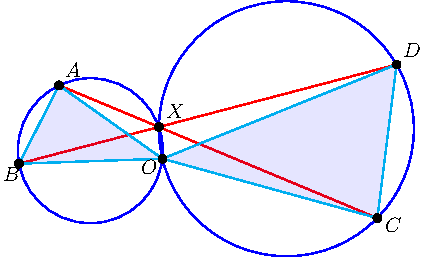
\includegraphics{spiral-lemma.pdf}
	\caption{Spiral Similarity Lemma}
\end{figure}

You may wonder that spiral similarity comes in pairs. As the next proposition says:
\begin{proposition}
The center of spiral similarity takin $AB$ to $CD$ is also the center of the spiral similarity taking $AC$ to $BD$.
\end{proposition}


\section{Miquel's Theorem}


\begin{theorem}[Miquel's Theorem]
Let $ABC$ be a triangle and $D,E,F$ eb the points on $BC,CA,AB$ respectively. Then the circumcircles of the triangles $AEF, BDF, CDE$ are concurrent.
\end{theorem}
\begin{figure}[ht]
\centering
	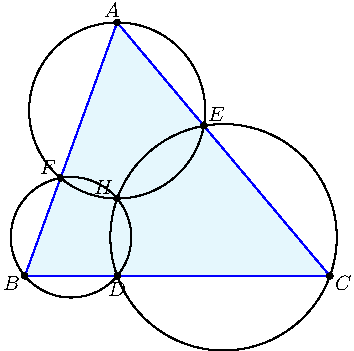
\includegraphics{miq-tri.pdf}
	\caption{Miquel's Theorem on $\triangle ABC$.}
\end{figure}
\begin{proof}
Let $(BDF) \cap (CDE)=H$.
Here we angle chase:
\[\angle EHF=\angle B +\angle C = 180 -\angle A.\]
done!
Another aproah is :
\[\angle AFH = \angle HDB, \angle AEH =\angle HDC.\]
which sum to $180\dg$.
\end{proof}
Note that $D,E,F$ can lie on the extension of the segments.


Here we are going to the Miquel's Quadrilateral Theorem which arise naturally.

\begin{theorem}[Miquel's (Quadrilateral) Theorem]
The four circles $(PAB), (PDC), (QAD), (QBC)$
concur at the Miquel point $M$. Furthermore, 
$M$ is the center of the spiral similarity sending
$AB$ to $DC$ and $BC$ to $AD$. (In particular,
 $ \triangle MAB \sim \triangle MDC$ and $\triangle MBC \sim \triangle MAD.$)
\end{theorem}
\begin{figure}[ht]
\centering
	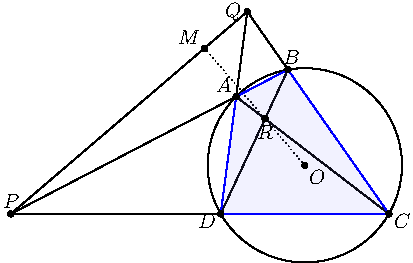
\includegraphics{miq-quad.pdf}
	\caption{Miquel's Theorem in Complete Quadrilateral.}
\end{figure}
The above theorem is same as the theorem for triangle's. Just consider thriangle $QDC$ and $P,A,B$ on the corresponding segments!

\begin{proof}
Let $M$ be the second intersection between $(QAB)$ and $(QCD)$ and by spiral similarity, $M$ is the center of the spiral similarity taking $AB$ to $CD$. SO, it is also the center of spiral similarity taking $BC$ to $DA$. By converse direction of the lemma $M$ lies on $(PAD)$ and $(ABC)$.
\end{proof}

Now we are going to see some properties of Miquel Point of a cyclic quadrilaral. It is known that \textit{One of the most powerful configurations in olympiad geometry is the Miquel point when
complete quadrilateral ABCD is cyclic}.

\begin{theorem}[Miquel's Theorem on a Cyclic Quadrilateral]
Miquel's Point has more properties in a cyclic quadrilateral. Beacuse of the fact that, $M$ is the inverse of $R$ (intersection of the diagonals) with respect to inversion around $(ABCD)$. 
\begin{itemize}
	\ii %$M$ is the common point of 
	The six circles $(OAC), (OBD), (P AD)$, $(P BC), (QAB),(QCD)$ goes through a single point i.e. $M$.
	\ii $M$ is the center of a spiral similarity taking $AB$ to $CD$, as well as the spiral similarity taking $BC$ to $DA$.
	\ii $M$ is the inverse of $R = AC \cap BD$ with respect to an inversion around $(ABCD)$. By Brocard’s theorem, $M$ is the foot of $O$ onto $PQ$.
	\ii $OM\perp PQ$.
\end{itemize}
\end{theorem}
These results also can be proved by angle chasing as well as spiral similarity. 

%\section{}











\chapter{Harder Divisibility}% by Atonu Roy Chowdhury}
\begin{linkb}
   \begin{itemize}
        \item \href{https://www.youtube.com/watch?v=kf_0msAOTMc}{Harder Divisibility(Atonu)} 
        \item \href{https://drive.google.com/file/d/1ZURQO2KSR9aaeaVyalL7GNuVBYhOGswB/view?usp=sharing}{1} , 
			\href{https://drive.google.com/file/d/1QHrhEnmAzimZjt-8k_T8AJrX3KiRSm73/view?usp=sharing}{2} 
   \end{itemize}
\end{linkb}

%\textbf{Prerequisities:}
\subsection*{Prerequisities:}
\begin{enumerate}
	\ii Residue System
	\ii Reduced Residue System
	\ii Fermat's Little Theorem(FLT: $a^{p-1}\equiv 1 \pmod p$ where $(a,p)=1$) and Euler's Theorem($a^{\varphi (m)}\equiv 1 \pmod m$ where $(a,m)=1$ and $m$ is not necessarily prime). 
	\ii Wilson's Theorem($p$ prime $\Leftrightarrow (p-1)! \equiv -1 \pmod p$)
\end{enumerate}
All of these topics are covered in Basic Divisibility Class: \autoref{sec:divi}.

\section{Order}
By Fermat's Little Theorem and Euler's Totient Function, 
$$a^{\varphi (m)}\equiv 1 \pmod m$$
If we are going to calculate
$a^1, a^2, a^3, \ldots, a^{\varphi (m)} \pmod m$ we find that, $a^n \equiv 1 \pmod m$ where $m< \varphi(m)$.

As an example $2^3 \equiv 1 \pmod 7$ but $2^{\varphi (7)} \equiv 2^6 \equiv 1 \pmod 7$

Here we find that $3$ is more special than $6$ in our example. Actually $3$ is order of $2$ modulo $7$.
Which is denoted by $\ord_{7}(2)=3$.

\begin{definition}[Order]
$\ord_{m}(a)=\min \{x:a^x\equiv 1 \pmod m \}$
\end{definition}
here a point to be noted that $\gcd (a,m)=1$.
If they aren't co-prime then no power of $a$ wil be $1$ modulo $m$.
Which is left as an exercise for the readers.

\begin{theorem}[Fundamental Theorem of Orders]
$\ord_m(a)=d$ then, $d|N \Leftrightarrow a^N \equiv 1 \pmod m$.
\end{theorem}
Let assume $N=dk$ and we know $a^d\equiv 1 \pmod m$ then, we have $a^{dk} \equiv 1 \pmod m$.

Assume for the sake of contradiction $d\not\mid N \implies N=dq+r $ such that $0<r<d$.
 Now, $a^d\equiv 1 \pmod m$. as $d$ is the order.
 Then we have $a^{dq}\equiv 1 \pmod m \implies a^N = a^{dq+r}\equiv 1 \cdot a^r \pmod m$
 \[\implies a^r \equiv 1  \pmod m \]
 which is a contradiction as $r$ can't be the order as $r<d$.

Here, we learn:
\begin{enumerate}
	\ii $d\mid \varphi_(m)$ which means $d\in \{ \mathrm{divisors of \varphi_(m)}\}$
	\ii $a^x\equiv a^y \pmod m \Leftrightarrow x\equiv y \pmod d$ where $\gcd(m,n) =1$.
	WLOG, $x\ge y$ so, $a^{x-y} \equiv 1 \pmod m$ then, $d\mid x-y $ and then we get $x\equiv y \pmod d$.

\end{enumerate}

\begin{example}
Given that $\gcd (a,m)=1$. Prove that $n\mid \varphi (a^n-1)$.
\end{example}
Let, $N=a^n-1$, so, $n\mid \varphi (N)$ and $\ord_N(a)\mid \varphi(N)$

So, we have to show that $a^n\equiv 1 \pmod N$

Assume for the sake of contradiction that, $k<n$ then we have, $a^k\equiv 1 \pmod N \implies N\mid a^k-1$

But, which means, $a^k-1 \ge N= a^n-1$

Contradiction as we assumed that $k<n$.

\begin{example}
Find all $n$ $n\mid 2^n-1$.
\end{example}
Here we find that $n$ must be odd and $n=1$ works. 
We let $n=2k+1$, so, $2k+1 \mid 2^{2k+1} -1$ 

Here we will use a lemma.
\begin{lemma}
If $a^x \equiv 1, a^y \equiv 1 $ all are taken modulo $m$. Then we have $a^{\gcd (x,y)} \equiv 1 \pmod m$
\end{lemma}

Let, $p$ be the smallest prime factor of $n$ (this trick is called the smallest prime factor(spf trick) of $n$)

$d=\ord_p(2)\implies d\mid \varphi(p)=p-1$
By FLT, $p\mid n \mid 2^n-1 \implies 2^n \equiv 1 \pmod p \implies d\mid n$ .

But then, 
\[ d\mid p-1, \ \ \ d\mid n \]
which is a contradiction! 
\section{Primitive Root}
\begin{definition}
Let $g$ is a positive integer and $\gcd(g,n)=1$. Then we shall call $g$ "Primitive Root modulo $m$" if $\ord_m(g)=\varphi(m)$.
\end{definition}
As an example, $\gcd(3,7)=1$, $3^6 \equiv 1 \pmod 7$.
We also know that $\varphi(7)=6$.
So, we can say that $3$ is a primitive root modulo $7$.

\begin{theorem}[Primitive Root]
Let, $p$ be a prime. Then $\exists g \in \{ 1,  \ldots, p-1 \}$ such that $g$ is a primitive root modulo $p$.
\end{theorem}
\begin{remark}
$\{1,\ldots, p-1\}$ is the reduced residue system of $p$ denoted by $RRS(p)$.
\end{remark}

\textbf{Usage and Properties of Primitive Root:}

%\begin{enumerate}
%	\ii
\begin{prop}
If $g$ is a primitive root modulo $m$ and $\varphi(m)$ is even then,$g^{\varphi(m)/2}\equiv -1 \pmod m$.
\end{prop}

Let, $\varphi(m)=2n$ So we have, \[g^{2n}\equiv 1 \pmod m \implies m\mid g^{2n}-1=(g^n+1)(g^n-1)\]
Which means, $m\mid g^n+1 $ or $m\mid g^n-1$.
So we have, $g^n\equiv -1$ or $g^n\equiv +1$ modulo $m$.

Now, AFTSOC (Assume for the sake of contradiction) that 
$g^n \equiv 1 \pmod m$
Then, $\varphi(m)=\ord_m(g)\le n$

But now we get $2n\le n$ which is absurd.

\begin{prop}
$S=\{ g, g^2, g^3, \ldots, g^{\varphi(m)} \}$ is $RRS(m)$ where $g$ is primitive root modulo $m$.
\end{prop}

%proof goes here



\section{Wilson's Theorem}

\begin{theorem}[Wilson's Theorem]
If $p$ is a prime then $(p-1)!\equiv -1 \pmod p$.
\end{theorem}
You can find a proof from Brilliant.org

\begin{problem}
Let $p$ be an odd prime. Find all $k$ such that \[p\mid 1^k + 2^k + 3^k +\ldots + (p-1)^k\]
\end{problem}
Here solving the above problem, you assume that you don't know any formula.

\chapter{Functional Equation}% by Raiyan Jamil}

\begin{linkb}
   \begin{itemize}
        \item \href{https://www.youtube.com/watch?v=7QhswMDYy0Y}{Functional Equation (Raiyan)}
        \item \href{https://drive.google.com/file/d/1KknJbbhPo3nK4ZneB3e22_bxlnGXF5j0/view}{Class} , \href{https://drive.google.com/file/d/1Kr_K2i_SQcefIWVR1yvgNN0Pnd3ZG0sg/view}{Chen}
        \item \href{https://drive.google.com/file/d/1cf1tifSEqKebrrDLyk2DONn0-0VlBSWs/view}{P set}
   \end{itemize}
\end{linkb}

(You can follow the note: \textit{Introduction to Functional Equation} by Evan Chen)



\section{Definitions}
Let $f : A \to B$ be a function.
The set $A$ is called the \vocab{domain}, and $B$ the \vocab{codomain}.
A couple definitions which will be useful:

\begin{definition}
	A function $f : A \to B$ is \vocab{injective} if $f(x) = f(y) \iff x=y$.
	(Sometimes also called \emph{one-to-one}.)
\end{definition}
\begin{definition}
	A function $ : A \to B$ is \vocab{surjective} if for all $b \in B$,
	there is some $x \in A$ such that $f(x) = b$.
	(Sometimes also called \emph{onto}.)
\end{definition}
\begin{definition}
	A function is \vocab{bijective} if it is both injective and surjective.
\end{definition}

\section{1st example}
\begin{example}
Find all functions $ f:\mathbb{R}\to\mathbb{R} $ such that $ f(f(x)^2+f(y)) = xf(x)+y $,$ \forall x,y\in R $.
\end{example}

Taking $x=y=0$, we see $f(a)=0$ for $a=f(0)^2+f(0)$. Taking $x=a$ gives $f(f(y))=y$, which means $f$ is bijective. Since $f$ is bijective, $f(a)=0=f(f(0))\implies f(0)=0$. Taking $y=0$ and $x\mapsto f(x)$ yields $f(x^2)=f(x)f(f(x))=xf(x)$. Swapping the sign on $x$, we see $f$ is odd. Making the replacements, $x\mapsto f(x)$, and $y\mapsto f(y)$, gives$$f(x^2+y)=xf(x)+f(y)=f(x^2)+f(y).$$Now let $x\ge 0$, and note that
\begin{align*}
f(x^2+2x+1)&=(x+1)f(x+1)\\
f(x^2)+2f(x)+f(1)&=(x+1)(f(x)+f(1))\\
f(x)&=xf(1)
\end{align*}But, $f$ odd extends this to all reals. Noting $f$ is involutive, we see that $f(1)=\pm 1$. This gives the solutions $\boxed{f=x}$ and $\boxed{f=-x}$

\section{Cauchy's Functional Equation}
\begin{theorem}[Cauchy's Functional equation over $\mathbb{Q}$]
If $ f(a)+f(b)=f(a+b) $ over $\mathbb{Q}$, then $f(x)=kx$ are only solutions for it. 
\end{theorem}
Let $f(1)=k$

Setting $x=y=0$, we get $f(0)=0$. and $x=y=1$, we get $2f(1)=f(2)=2k$.
Now setting $(x,y)=(x,1)$, we get $f(x)+f(1)=f(x+1) \implies f(x+1)=kx+k=k(x+1)$, so we are done for integers.

We can show that $q\times f(\frac{p}{q})=(p)=kp$.

from where we get that $f(p/q)=\frac{kp}{q}$ and we are done over $\mathbb{Q}$

\begin{example}[IMO 2019 P1]
Let $\mathbb{Z}$ be the set of integers. Determine all functions $f: \mathbb{Z} \rightarrow \mathbb{Z}$ such that, for all integers $a$ and $b$,$$f(2a)+2f(b)=f(f(a+b)).$$
\end{example}
Set $a = 0$ to get $f(f(b)) = 2f(b) + f(0)$. Thus the given rewrites as $f(2a) + 2f(b) = 2f(a + b) + f(0)$. Now let $a = b$ to get $f(2a) = 2f(a) - f(0)$, so the given becomes $f(a) + f(b) = f(a + b) + f(0)$. Letting $g(x) = f(x) - f(0)$ this is just $g(a + b) = g(a) + g(b) $ over integers, implying cauchy, we get $g(x) = kx$ and $f(x) = kx + f(0)$

Now doing some substitutions, we get $k=2$
So, either $f(x)=0$ for all $x$ or $f(x)=kx+c$ 
\begin{theorem}[Cauchy + Continuous $\implies$ Linear]
	Suppose $f : \RR \to \RR$ satisfies $f(x+y) = f(x) + f(y)$.
	Then $f(qx) = qf(x)$ for any $q \in \QQ$.
	Moreover, $f$ is linear if any of the following are true:
	\begin{itemize}
		\ii $f$ is continuous in any interval. 
		\ii $f$ is bounded (either above or below) in any nontrivial interval.
		\ii There exists $(a,b)$ and $\eps > 0$ such that $(x-a)^2 + (f(x)-b)^2 > \eps$ for every $x$
		(i.e.\ the graph of $f$ omits some disk, however small).
	\end{itemize}
\end{theorem}

\begin{example}
Find all continuous function $f: \RR \to \RR$ such that $$f(x+y)-f(x)-f(y)=xy(x+y)$$
\end{example}

\begin{example}[Field Automorphisms of $\RR$]
	Solve over $\RR$:
	\[ f(x+y) = f(x) + f(y) \quad\text{and}\quad f(xy) = f(x)f(y). \]
\end{example}
\begin{proof}
	[Solution]
	We claim $f(x) = x$ and $f(x) = 0$ are the only solutions (which both work).
	According to the theorem, to prove $f$ is linear it suffices to show $f$ is nonnegative
	over some nontrivial interval.
	Now, \[ f(t^2) = f(t)^2 \ge 0 \] for any $t$,
	meaning $f$ is bounded below on $[0,\infty)$
	and so we conclude $f(x) = cx$ for some $c$.
	Then $cxy = (cx)(cy)$ implies $c \in \{0,1\}$, as claimed.
\end{proof}

\section{Some intuitions and motivations}
\begin{example}[Cancelling the stuffs]

	Solve over $\RR$: \[ f(x^2+y) = f(x^{27} + 2y) + f(x^4). \]
\end{example}
\begin{soln}
	For this problem, we claim the only answer is the constant function $f=0$.
	As usual our first move is to take the all-zero setting, which gives $f(0) = 0$.

	Now, let's step back: can we do anything that will make lots of terms go away?
	There's actually a very artificial choice that will do wonders.
	It is motivated by the \vocab{battle cry}:
	\begin{quote}
		\itshape ``DURR WE WANT STUFF TO CANCEL.''
	\end{quote}
	So we do the most blithely stupid thing possible.
	\emph{See that $x^2+y$ and $x^{27}+2y$ up there?}
	Let's make them equal in the rudest way possible:
	\[ x^2 + y = x^{27} + 2y \iff y = x^2 - x^{27}. \]
	Plugging in this choice of $y$,
	this gives us $f(x^4) = 0$, so $f$ is zero on all nonnegatives.

	All that remains is to get $f$ zero on all reals.
	The easiest way to do this is put $y=0$ since this won't 
	hurt the already positive $x^2$ and $x^4$ terms there.
\end{soln}
This is a common trick: see if you can make a substitution that will kill off two terms.

\begin{example}[Finding a constant term]
	\label{ex:singapore}
	Solve over $\RR$:
	\[ (x-y)f(x+y) - (x+y)f(x-y) = 4xy(x^2-y^2). \]
\end{example}
\begin{soln}
	First of all, the $x-y$ and $x+y$ everywhere are a mess,
	so we replace them with $a = x+y$ and $b = x-y$
	(this doesn't lose any information).
	Then $x^2-y^2 = ab$, and also $2x = a+b$, $2y = a-b$.
	So, the equation is just saying that
	\[ bf(a) - af(b) = ab(a^2-b^2). \]

	Plugging  $a=0$ is fruitful: we derive
	$bf(0) = 0$, so $f(0) = 0$.
	
	Next, assume $a,b \neq 0$.
	We do the following nice trick:
	if we divide by $ab$, we obtain
	\[ \frac{f(a)}{a} - \frac{f(b)}{b} = a^2 - b^2. \]
	You'll notice that the $a$ and $b$ terms are completely isolated now!
	That is, we can write
	\[ \frac{f(a)}{a} - a^2 = \frac{f(b)}{b} - b^2. \]
	This is enough to imply that $\frac{f(a)}{a} - a^2 = c$ for some constant $c$,
	whenever $a \neq 0$; hence $f(x) = x^3 + cx$ for some $c$.
	Initially we only know this for $x \neq 0$,
	but it holds for $x=0$ as well since $f(0) = 0$.

	And now, we observe that these solutions all work, and we're done.
\end{soln}

\section{Three More Tricks}
Here are three more tricks that are frequently useful.

\begin{itemize}
	\ii \vocab{Tripling an involution}.
	If you know something about $f(f(x))$,
	try applying it $f(f(f(x)))$ in different ways.
	For example, if we know that $f(f(x)) = x+2$,
	then we obtain $f^3(x) = f(x+2) = f(x)+2$.

	\ii \vocab{Isolated parts}.
	When trying to obtain injective or surjective,
	watch for ``isolated'' variables or parts of the equation.
	For example, suppose you have a condition like
	\[ f(x+2xf(y)^2) = yf(x) + f(f(y)+1) \]
	
	Noting that $f \equiv 0$ works, assume $f$ is not zero everywhere.
	Then by taking $x_0$ with $f(x_0) \neq 0$,
	one obtains $f$ is injective.
	(Try putting in $y_1$ and $y_2$.)

	Proving surjectivity can often be done in similar spirit.
	For example, suppose
	\[ f(f(y)+xf(x)) = y+f(x)^2. \]
	By varying $y$ with $x$ fixed we get that $f$ is surjective,
	and thus we can pick $x_0$ so that $f(x_0) = 0$
	and go from there.
	Surjectivity can be especially nice if every $y$
	is wrapped in an $f$, say; then each $f(y)$ just becomes
	replace by an arbitrary real.

	\ii \vocab{Exploiting ``bumps'' in symmetry}.
	If some parts of an equation are symmetric and others are not,
	swapping $x$ and $y$ can often be helpful.
	For example, suppose you have a condition like
	\[ f(x+f(y)) + f(xy) = f(x+1)f(y+1) - 1 \]

	This equation is ``almost symmetric'',
	except for a ``bump'' on the far left where $f(x+f(y))$ is asymmetric.
	So if we take the equation with $x$ and $y$ flipped
	and then eliminate the common terms,
	we manage to obtain \[ f(x+f(y)) = f(y+f(x)). \]
	If we've shown $f$ is injective, we are even done!
	So often these ``bumps'' are what let you solve a problem.
	(In particular, don't get rid of the bumps!)
\end{itemize}


\section{Practise Problems}
\begin{problem}
Find all continuous functions $f: \mathbb{R} \to \mathbb{R}$ such that $$f(f(x+y))=f(x)+f(y)$$
\begin{hint}
\addhint{plugging in $(x+y,0)$ helps}
\addhint{Find $f(0)$}
\addhint{use cauchy}
\end{hint}
\end{problem}

\begin{problem}
Find all functions $f: \mathbb{R} \to \mathbb{R}$ such that $$f(f(x+y))=f(x+y)+f(x)f(y)-xy$$ for all $x,y \in \mathbb{R}$
\begin{hint}
\addhint{}
\end{hint}
\end{problem}

\begin{problem}
Find all functions $f: \mathbb{R} \to \mathbb{R}$ such that $$f(x+2y)=f(x)(2y+1)+f(xy)$$ for all $x,y \in \mathbb{R}$
\begin{hint}
\addhint{}
\end{hint}
\end{problem}

\begin{problem}
Find all continuous functions $f: \mathbb{R} \to \mathbb{R}$ such that $$f(x+af(y))=f(x+y)+(a-1)y$$ for $a\neq 0,1$ is a constant.
\begin{hint}
\addhint{}
\end{hint}
\end{problem}
\begin{problem}
Find all functions $f: \mathbb{R} \to \mathbb{R}$ such that $$f(x^2+y)=f(f(x)-y)+4f(x)y$$ for all $x,y \in \mathbb{R}$
\begin{hint}
\addhint{}
\end{hint}
\end{problem}




%%%%%%%%%%%%%%%%%%%%%%%
\chapter{Combinatorics TSTST}\label{tstst:combi}
%\chapter{April 30, 2021}
%\begin{center}
%\LARGE{THIS IS OUR OFF DAY} 

%\LARGE{:D}

%\end{center}

%Problems---
%Exam-1 Problems
%\includepdf[pages=-]{exam1.pdf}
The Combinatorics Exam of The National Camp.
Problems are given below:

\begin{prob}\label{combi:1}
You have a set $S$ of $19$ points in the plane such that given any three points in $S$, there exist two of them
whose distance from each other is less than $1$. Prove that there exists a circle of radius $1$ that encloses
at least $10$ points of $S$.
	\begin{hint}
	\addhint{Start with Pigeon-hole Principle!}
	\addhint{}
	\end{hint}
\end{prob}

\begin{prob}\label{combi:2}
There are $2021$ stones in a pile. At each step, Lazim chooses a pile with at least two stones, splits it into
two piles, and multiplies the sizes of the resulting two piles. He keeps doing this until there are $2021$
piles each containing exactly one stone. Finally, he adds up all the products he has obtained during the
process and ends up with the number $N$ . Find, with proof, all the possible values of $N$ .
	\begin{hint}
	\addhint{}
	\addhint{}
	\end{hint}
\end{prob}

\begin{prob}\label{combi:3}
Show that for all positive integers $n\ge 2$, you can cut any quadrilateral into $n$ isosceles triangles.
	\begin{hint}
	\addhint{Induction!}
	\addhint{}
	\end{hint}
\end{prob}

\begin{prob}\label{combi:4}
Let $n \ge 1$ be an integer. A non-empty set is called “good” if the arithmetic mean of its elements is an
integer. Let $T_n$ be the number of good subsets of $\{1, 2, 3 \ldots , n\}$. Prove that for all integers $n$, $T_n$ and $n$
leave the same remainder when divided by $2$.
	\begin{hint}
	\addhint{}
	\addhint{}
	\end{hint}
\end{prob}

\begin{prob}\label{combi:5}
We place some checkers on an $n \times n$ checkerboard so that they follow the conditions:
	\begin{itemize}
		\ii every square that does not contain a checker shares a side with one that does;
		\ii given any pair of squares that contain checkers, we can find a sequence of squares occupied by
		checkers that start and end with the given squares, such that every two consecutive squares of the
		sequence share a side.
	\end{itemize}
Prove that at least $(n^2-2)/3$ checkers have been placed on the board.
	\begin{hint}
	\addhint{Extremal Combinatorics!}
	\addhint{Call a square good if it contains a checker or shares a side with a square containing a checker.}
	\addhint{We don't know how much contribution a checker has. }
	%\addhint{So, we should not }
	\addhint{So, we start adding checkers. Suppose that $k$ checkers will be added.}
	\addhint{Place one checker on the board to start, and then in each step place one checker adjacent to one that has already been placed.}
	\addhint{In first step, after adding $2$ checkers, at most $5$ squares become good.}
	\addhint{In each step, at most $3$ square which were not already good, become good.}
	\addhint{So, $5+3(k-2) = 3k+2$ and hence, $n^2 \le 3k+2$.}
	\end{hint}
\end{prob}


Full Solutions to these problems can be found at \autoref{sols:tstst}.

\chapter{Length Chase}% by Raiyan Jamil}

\begin{linkb}
   \begin{itemize}
        \item \href{https://www.youtube.com/watch?v=_JJuNoIr_v4}{Length Chase (Raiyan)}
        \item \href{https://drive.google.com/file/d/1SWvcvf99adDs0YVglds3kCpvHxeTdLqP/view}{Things are ...} 
        \item \href{https://drive.google.com/file/d/1MocEDGQHzkW7vjUj6n6HXa_m3iBQRwmG/view}{P set} 
   \end{itemize}
\end{linkb}

\section{Ceva's and Menelaus's Theorem}

A line through a vertices connecting a point on the opposite side of a vertex is called a \textbf{cevian}.

Three cevian may concurrent or not. It is detremined my the ceva's theorem. 
\begin{theorem}[Ceva's Theorem]
Let $D,E,F$ be arbitrary points on the line $BC,CA,AB$. $AD,BE,CF$ are concurrent if and only if \[\frac{BD}{DC}\cdot \frac{CE}{EA}\cdot \frac{AF}{FB}=1.\]
\end{theorem}
\begin{figure}[ht]
\centering
	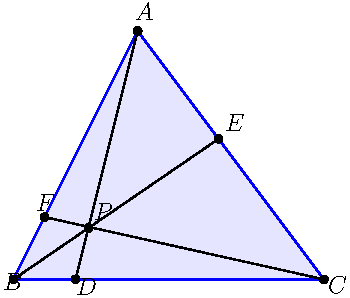
\includegraphics{ceva.pdf}
	\caption{Ceva's Theorem}
\end{figure}
You can prove the formula using areal ratios.

\begin{theorem}[Menelaus's Theorem]
Let $D,E,F$ be arbitrary points on the line $BC,CA,AB$. $D,E,F$ are collinear if and only if \[\frac{BD}{DC}\cdot \frac{CE}{EA}\cdot \frac{AF}{FB}=-1.\]
where the distances are directed.
\end{theorem}
Same as above.

\section{Trigonometric Ceva's Theorem}
\begin{theorem}[Trigonometric form of Ceva's Theorem]
Let $D,E,F$ be arbitrary points on the line $BC,CA,AB$. $AD,BE,CF$ are concurrent if and only if \[\frac{\sin \angle BAD}{\sin \angle DAC}\cdot \frac{\sin \angle CBE}{\sin \angle EBA}\cdot \frac{\sin \angle ACF}{FCB}=1.\]
\end{theorem}
For proving the formula, you have to use the fact that $\triangle ABC$ has area $=\half AB \cdot AC \sin BAC$.

\section{Isotomic Conjugate}
Let $D$ be a point on the line $BC$ and $M$ eb the midpoint o the line segment. $M'$ be the reflection of $D$ over $M$. Then, $AD'$ is called the isotomic of $AD$. 


\begin{theorem}[Isotomic Conjugate]
Let $AD,BE,CF$ are concurrent cevians of a triangle $ABC$. Then the isotomics $AD'$, $BE'$, $CF'$ are also concurrent. The point of concurrency is called the Isotomic Conjugate of the first one.
\end{theorem}

\begin{figure}[ht]
\centering
	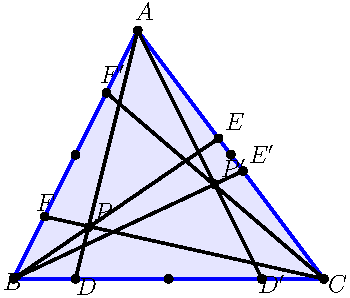
\includegraphics{isotomic.pdf}
	\caption{Isotomic conjugate $P'$.}
\end{figure}

\section{Isogonal Conjugate}
Let $AD$ be a cevian of $ABC$. Angle bisector of $\angle BAC$ is $AI$. Then, the reflection of the line $AD$ over $AI$ is called the isogonal of $AD$.
\begin{theorem}[Isogonal Conjugate]
Let $AD,BE,CF$ are concurrent cevians of a triangle $ABC$. Then the isogonals $AD',BE',CF'$ are also concurrent. The point of concurrency is called the Isogonal Conjugate of the first one.
\end{theorem}
\begin{figure}[ht]
\centering
	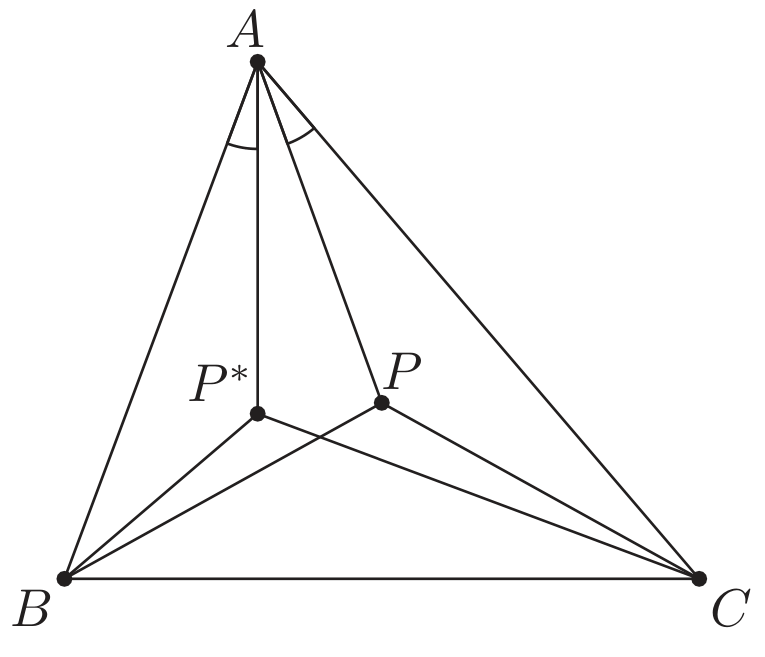
\includegraphics[scale=0.5]{isogonal-conj.png}
	\caption{Isogonal Conjugate of $P$.}
\end{figure}
\section{Projective Plane}
Here is a long discussion.

I write in a brief.

The summary of the discussion is:
\begin{enumerate}
	\ii There are infinitely many points at infinity.
	\ii There is exactly 1 line at infinity.
	\ii All points at infinity lie on the line at infinity.
\end{enumerate}
\[\mathbf{Projective \ Geometry = Euclidean \ Geometry + point \ at \ \infty + line \ at \ \infty }\]
There is an another perspective.

\textbf{Line at infinity is a circle with radius $\infty$ which goes htrough all the points at infinity.}

\chapter{NT Functions}% by Ahsan Al Mahir}

\begin{linkb}
   \begin{itemize}
        \item \href{https://www.youtube.com/watch?v=BIocWacBJEs}{Number Theory Functions (Lazim)}
        \item \href{https://drive.google.com/file/d/1pedr_KX0Yom8O2hremeRoJO13zhEeEmY/view}{Class Note}
   \end{itemize}
\end{linkb}

What is NT Function? Number Theoretic Function is a function which has Co-domain $\NN$. Some common tricks for solving such functions are,
\begin{itemize}
 \item Attempt to prove that the function is linear. (Proving $f(x) = ax + b $ for some constant $a,b$.). 
 \item Use induction.
 \item If a number is divided by infinitely many primes then the number is $0$
 \item Always look if you can eliminate something. 
 \item Try prime numbers, 1, n-1 or some large numbers-small numbers and so on.
 \end{itemize} 
\section{Some Techniques}
 \begin{theorem}[Cauchy's functional equation]
 If, 
\[ f(x) + f(y) = f(x+y) \]
 for all $x,y\in \mathbb Q $. Then $f(x) = cx$. $c$ is a constant such that $c\in \mathbb Q$
\end{theorem}
This is useful as we can use Cauchy in Number theory functions.
 
 Another tip for practicing nt functions is practicing a lot of construction problems.
 Dirichlet theorem is often useful, The weak version of this theorem is,
 \begin{theorem}[Dirichlet theorem]
 For $gcd(a,b) = 1$, there are infinitely many primes in the form of $an+b$, where n is variable.
 \end{theorem}
 However this is not easy to prove. Interested reader may look up the proof on internet/books.
\section{Solving Some IMO SL Problems}

 
 \begin{example}[IMO SL-2010/A1]
 Find all function $f:\mathbb{R}\rightarrow\mathbb{R}$ such that for all $x,y\in\mathbb{R}$ the following equality holds
 \[ f(\left\lfloor x\right\rfloor y)=f(x)\left\lfloor f(y)\right\rfloor \]
 where $\left\lfloor a\right\rfloor $ is greatest integer not greater than $a$.
 
 \end{example}
\begin{soln}
Desired functions are, $f(x) = 0$, $f(x) = c$ where $1\le c < 2 $

let $P(x,y) \implies f(\left\lfloor x\right\rfloor y)=f(x)\left\lfloor f(y)\right\rfloor $
(this is also known as assertion). 

Now, \[P(0,0) \implies f(0) = f(0).\left \lfloor f(0) \right \rfloor \implies f(0) = 0 \text{ or }  \left\lfloor f(0) \right \rfloor = 1\]
\textbf{Case 1:} $\left\lfloor f(0) \right \rfloor = 1 $. Then,


\[P(0,y) \implies f(0) = f(0)\left\lfloor f(y)\right\rfloor \implies \left\lfloor f(y)\right\rfloor = 1 \]
For all $y\in \mathbb R $.
$\therefore 1 \le  f(y) < 2   $
Now back to the main function.
Notice, 
\[f(\left\lfloor x\right\rfloor y) = f(x)  \]
Plug in $y= \frac{y}{\left\lfloor x\right\rfloor} $. Then,
$f(y)=f(x)$ for all $x,y \in \mathbb R$.

$\therefore f$ must be a constant function. Means $f(x) = c $.Since $\left\lfloor f(y)\right\rfloor = 1$,  Hence, $1 \le  c < 2  $. Which is a solution of this function. One can easily verify.

\textbf{Case 2: } f(0)= 0

We observe some assertions, 
$P(1,1) \implies f(1) = f(1)\left\lfloor f(1) \right \rfloor \implies f(1) = 0 \text { or } \left\lfloor f(1) \right \rfloor= 1 $


\textbf{Sub-case 1: }  $f(1) = 0$.

$ P(1,y) \implies f(y) = f(1) \left \lfloor f(y) \right \rfloor  \implies f(y) = 0$ for all real $y \in \mathbb R$.
This is another solution which satisfies the given functional equation.


\textbf{Sub-case 2: } $\left\lfloor f(1) \right \rfloor= 1 $


%Then, $\left\lfloor f(1) \right \rfloor \implies = 0 $. 
 $P(x,1)$ gives, $f(\left\lfloor x\right\rfloor) = f(x)$. 
 Now let $n \in \mathbb N$ ($y $ is a real number). Then, $f(ny) = f(n) \left\lfloor f(y) \right\rfloor $. Set, $y = \frac{1}{n}  $. Then,
 \[\ f(1) = f(n) \left\lfloor f\left (\frac{1}{n} \right) \right\rfloor =f(n) \left\lfloor f\left (\left\lfloor \frac{1}{n} \right\rfloor \right  ) \right\rfloor = f(n)\left\lfloor f(0) \right\rfloor  = 0.  \]
But, $\left\lfloor f(1) \right \rfloor= 1 $ so $f(1) \ne 0$. So contradiction.
No functions exist in this condition.
\end{soln}



\begin{example}[IMO SL 2019/N4]
Find all functions $f:\mathbb Z_{>0}\to \mathbb Z_{>0}$ such that $a+f(b)$ divides $a^2+bf(a)$ for all positive integers $a$ and $b$ with $a+b>2019$.
\end{example}


\begin{soln}
Let $P(x,y)$ be the assertion.
\[P(1, n) \implies 1 + f(n) \mid 1 + nf(1)  \]
By Dirichlet theorem, we can have $1 + nf(1)$ a prime number for infinitely many $n$.

$\therefore 1 + f(n) = 1 + nf(1) $ . So, $f(n) = nf(1)$ for infinitely many n.
Now we take such $n$ and any positive integer $a$ .
\[P(a,n) \implies (a+ f(n)) \mid  (a^2 + nf(a))\]
\[ \implies a+ nf(1) \mid  a^2 + nf(a )\]
\[ \implies a+ nf(1)\mid f(1)(a^2 + nf(a )) - f(a)(a+ nf(1))\]
\[ \implies a+ nf(1)\mid  a^2f(1) -a f(a )\]

But we can take really big $n$. So, $a^2f(1) -a f(a)$ has to be $0$. So,  $f(a) = af(1)  $. 

$f(1) $ can be any integer $\in \mathbb Z_{>0}$. It is easy to verify that this funtion satisfies the given equation. And we are done!

\end{soln}














\section{Practise Problems}



























\chapter{Quadratic Residue and Diophantine Equation}% by Atonu Roy Chowdhry}
\begin{linkb}
   \begin{itemize}
        \item \href{https://www.youtube.com/watch?v=YeurXbh2sIQ}{Video 1} + \href{https://www.youtube.com/watch?v=3ZBGv6dH37o}{Video 2}
        \item \href{https://drive.google.com/file/d/1lHBgt42uKI6qc0-Yt_Sx7boahxsYLVN7/view}{An Intro ...(book)}, \href{https://drive.google.com/file/d/12nate-JVlXwJUkMS7ja6ftBvyTWatace/view?usp=sharing}{Class note}
        
        \item \href{https://drive.google.com/file/d/16tC_XxRU31j_iOVZ3gEb_BMcZlQBfIP7/view?usp=sharing}{Note + P Set}
   \end{itemize}
\end{linkb}
\section{Quadratic Residue}

(Note: here \textit{qr} means quadratic residue)

\begin{definition}[Quadratic Residue]
$a$ is called quadratic residue modulo $n$ if $\exists x: x\equiv a \pmod n$. 
\end{definition}

\begin{definition}[Quadratic Residue Class]
$qr(n)=\{a:a \mathrm{is \ a \ qr \ in \ mod} n \}$.
\end{definition}
As an example $qr(5)=\{0,1,4\}$.

\begin{theorem}
If $-1$ is a qr in mod $p$ where $p$ is an odd prime. Then, $ p \equiv 1 \pmod 4$.
\end{theorem}

AFTSOC, $p\equiv -1 \pmod 4$ or $p = 4k-1$.
So $\exists x : x^2\equiv -1 \pmod p$. 
\[x^{p-1}\equiv 1 \pmod p \ \mathrm{By FLT}\]
\[\implies x^{4k-2}\equiv 1\pmod p\]
\[\implies (x^2)^{2k-1}\equiv 1 \pmod p\]
\[\implies (-1)^{2k-1}\equiv 1 \pmod p\]
\[-1\equiv 1 \pmod p\]
which is absurd.

The converse of the above theorem is also true.
\begin{theorem}
If $ p \equiv 1 \pmod 4$ is a prime then -1 is a quadratic residue mod $p$
\end{theorem}
The proof is constructive\ldots


\section{Legendre's Formula}
\begin{definition}[Legendre Symbol]
\[\left(\frac{n}{p}\right)=\begin{cases}
				0 & p\mid n \\
				1 & n\in qr(p) \\
				-1 & n\not\in qr(p)
				\end{cases}
				\]
\end{definition}

\begin{theorem}
\[a^{\frac{p-1}{2}}\equiv \left(\frac{a}{p}\right) \pmod p \]
\end{theorem}


\begin{lemma}
\[\left(\frac{ab}{p}\right)=\left(\frac{a}{p}\right)\left(\frac{b}{p}\right)\]
\end{lemma}
The meaning of the above lemma is if $a,b$ are both qr then $ab$ is also qr.

If $a,b$ both are not qr then $ab$ is a qr.

But, if only one of them is qr, then, $ab$ is not qr.

\begin{lemma}
\[\left(\frac{-1}{p}\right)=\begin{cases}
			-1 & p=4k+1 \\
			1 & p=4k-1
			\end{cases}
			\]
\end{lemma}

\begin{lemma}
\[\left(\frac{2}{p}\right)=(-1)^{\frac{p-1}{8}}\]
\end{lemma}


\begin{lemma}
\[\left(\frac{p}{q}\right)\left(\frac{q}{p}\right)=(-1)^{\frac{p-1}{2}}\cdot (-1)^{\frac{q-1}{2}}\]
\end{lemma}
\textbf{Techniques:}
Whenever you see squares you should take moulo $2^n$.

\section{Diophantine Equation}
Here we are going to solve some diophantine equation problems (i.e. problems asking for integer solutions)
\begin{example}
$d\neq 2,5,13$, $S=\{2,5,13,d\}$. Prove that, $\exists a,b \in S$ such that $ab-1 \neq k^2$
\end{example}
Here you have to show that there is no such $d$ that satisfies all the equations:
\begin{align*}
2d-1 &=x^2 \\
5d-1 &=y^2 \\
13d-1 &=z^2 
\end{align*}

AFTSOC, exists such $d$.  
First take mod $4$,

$qr(4)=\{0,1\}$

So, $2d-1 \pmod 4 \in \{0,1\}.$ Here, $2d-1$ doesn't congruent to 0 modulo $4$ as it is odd.

So, $2d-1 \equiv 1 \pmod 4 \implies d\equiv 1 \pmod 2$

But, then mod $4$ and mod $8$ aren't useful. Then take mod 16. Then some exercise left for the readers.


%\paragraph{What if power $\ge 2$?}
\begin{example}
Find all solutions to the equation:
\[x^3 + y^4 =7\]
\end{example}
Here we need to find a prime $p$ such that $3|p-1$ and $4|p-1$. 
$p=13 $ is a good choice.

So we work with mod $13$. We get:
$x^3 \pmod {13} =\{0,1,5,8,12\}$ and $y^4 \pmod {13} = \{0,1,3,9\}$.

But no such summation of two elements from the sets is equal to $7$. So, there is n such solution.

\begin{example}
Find all solutions to the equation:
$$x^5-y^2=4$$
\end{example}
Here the magical mod is $11$.
We get $x^5 \pmod {11} =\{0,1,-1\}$. And $y^2=x^5-4 \pmod {11} =\{6,7,9\}$

But quadratic residue $\pmod {11} =\{0,1,4,9,5,3\}$.

So, there is no such solution.

\section{Practise Problems}

\begin{problem}


	\begin{hint}
	\addhint{}
	\addhint{}
	\end{hint}
\end{problem}

\begin{problem}


	\begin{hint}
	\addhint{}
	\addhint{}
	\end{hint}
\end{problem}

\begin{problem}


	\begin{hint}
	\addhint{}
	\addhint{}
	\end{hint}
\end{problem}

\begin{problem}


	\begin{hint}
	\addhint{}
	\addhint{}
	\end{hint}
\end{problem}

\begin{problem}


	\begin{hint}
	\addhint{}
	\addhint{}
	\end{hint}
\end{problem}

\begin{problem}


	\begin{hint}
	\addhint{}
	\addhint{}
	\end{hint}
\end{problem}

\begin{problem}


	\begin{hint}
	\addhint{}
	\addhint{}
	\end{hint}
\end{problem}

\chapter{Inequality}% by Zim-mim Siddiqee Sowdha}
\begin{linkb}
   \begin{itemize}
        \item \href{https://www.youtube.com/watch?v=H7UwnAGZY0A}{Inequality (Sowdha)} 
        \item \href{https://drive.google.com/file/d/1Vm117lBF5yuZrRGMjmMS-HccPmknl5uK/view?usp=sharing}{Apply AM-GM ...}
        \item \href{https://drive.google.com/file/d/12GWPOw5_9c4-KD5PNCdJSS0i3lAORI5s/view}{P set}
   \end{itemize}
\end{linkb}
%\section{Some Theorems and Lemmas}
\section{Triangle inequality}
 In euclidean geometry,for any triangle with side $a$, $b$,$c$,
 \[a+b >c\] 
and \[a-b<c\] and so on.

In vector space the triangle inequality also holds. Which means, when $a$ and $b $ are vectors then,
\[|a+b| \le |a|+|b|\]
 and \[|a-b|\ge ||a|-|b||\]
 
  This is true for any real number $a$ and $b$ where $|a|$ is the absolute value of $a$. Because, 
  \[ (a+b)^2 = |a|^2+ |b|^2 + 2ab \le |a|^2 + 2|a||b| + |b|^2 = (|a|+|b|)^2  \]
  \[\implies |a+b|^2 \le  (|a|+|b|)^2 \]
  \[\implies |a+b| \le  (|a|+|b|) \]
  The other one can be proved similarly. 
 
 
    \section{Some classic definitions of means}
    \begin{definition}[Root Mean Square]
    Root mean square of $a_1, \cdots ,a_n$ positive real numbers defined as,
    \[\sqrt {\frac{a_1^2+ \cdots +a_n^2}{n}}\]
    This is also known as quadratic mean.
    \end{definition}
\begin{definition}[Arithmetic Mean ]
Arithmetic mean of $a_1, \cdots ,a_n$ positive real numbers defined as, 
\[ \frac{a_1+...+a_n}{n}\]
\end{definition}
\begin{definition}[Geometric Mean]
Geometric mean of $a_1, \cdots  ,a_n$ positive real numbers defined as, 
   \[ (a_1 \cdots a_n)^{\frac{1}{n}} \]
\end{definition}
\begin{definition}[Harmonic Mean]
Geometric mean of $a_1, \cdots  ,a_n$ positive real numbers defined as,
\[\frac{n}{\frac{1}{a_1}+\cdots+ \frac{1}{a_n}}\]
\end{definition}
  
 \begin{theorem}[RMS-AM-GM-HM inequality]
 For positive reals $a_1, \cdots  ,a_n$ we have
        \[\sqrt {\frac{a_1^2+ \cdots +a_n^2}{n}} \ge \frac{ a_1+...+a_n}{n} \ge (a_1 \cdots a_n)^{\frac{1}{n}} \ge \frac{n}{\frac{1}{a_1}+\cdots+ \frac{1}{a_n}} \]
 \end{theorem}
%\begin{theorem}[Triangle inequality]
%for 2 vectors $a$ and $b$, 
%\[|a+b|\le|a|+|b|\]
%\end{theorem}
 %   This inequality is true for all real number $a, b$%
 
\section {A fun proof of RMS-AM-GM-HM}
We present a geometric proof of RMS-AM-GM-HM inequality for $n=2$.Let $a,b $ be two real numbers then. Consider the following diagram,
\begin{figure}[ht]
\centering
    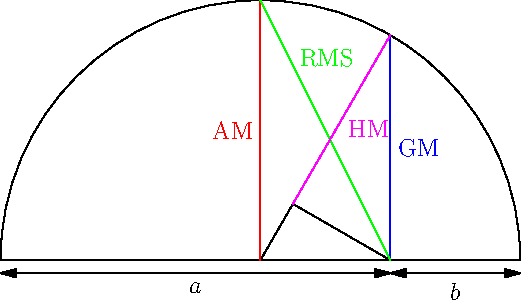
\includegraphics{am-gm.pdf}
    \label{label of the figure}         
\end{figure}
It is left as an exercise to figure out why this lines refer to the corresponding meaning. 
Now it is easy to see that why this inequality is true for $n=2$. 

\section{Example Problems}

\begin{example}
$\frac{m}{n}<\sqrt{2}$ if and only if  $\sqrt{2} < \frac{m+2n}{m+n}$

\end{example}
\begin{soln}
    For the if part, \[ \frac{m}{n}<\sqrt{2} \]
    \[ \implies  \frac{m}{n} +1 < \sqrt{2} +1\]
    \[ \implies \frac{1}{\frac{m}{n} +1 }> \frac{1}{\sqrt{2}+1} \]
    \[ \implies 1 + \frac{1}{\frac{m}{n} +1 }> 1 +\frac{1}{\sqrt{2}+1} \]
    \[ \therefore \frac{m+2n}{m+n} > \sqrt {2} \]
    For the only if part, just go backwards. Which completes the proof.
\end{soln}


\begin{example}
$x,y,z $ are positive real numbers. Prove that,
\[\frac{xy}{z}+\frac{yz}{x}+\frac{zx}{y}\ge x+y+z\]
\end{example}
 \begin{soln}
 Here by AM-GM, we get ,
 \[\frac{xy}{z}+\frac{yz}{x}\ge 2 \sqrt {\frac{xy.yz}{z.x}}= 2y\]
 Similarly,
 \[\frac{yz}{x}+\frac{zx}{y}\ge 2z\]
     \[ \frac{zx}{y}+\frac{xy}{z} \ge 2x\]
     Then add these 3 inequalities will give the desired inequality. And we are done!
 \end{soln}
\begin{example}
Let $x,y $ be positive integers. Prove that, 
\[\frac{1}{x} + \frac{1}{y} \ge \frac{4}{x+y}\]
\end{example}

\begin{soln}
Notice that by AM-GM we get, 
\[(x+y) \ge 2 \sqrt{xy}\]
\[\implies (x+y)^2 \ge 4xy\]
Now multiply both side with $\frac{1}{xy(x+y)} $
\[\frac{x+y}{xy} \ge \frac{4}{x+y}\]
\[\implies \frac{1}{x} + \frac{1}{y} \ge \frac{4}{x+y}\]
Which is exactly what we wanted!

\end{soln}
However there is an another solution of this problem,
\begin{soln}
Take $a=\frac{x+y}{x}, b = \frac {x+y}{y}$. 
Now, by AM-GM we get, 
\[ a+b\ge 2\sqrt{ab}\]
\[\implies \frac{x+y}{x} + \frac{x+y}{y}\ge 2\sqrt{\frac{(x+y)^2}{xy}}=\frac{2(x+y)}{\sqrt{xy}} \]
Since, $x+y\ge 2\sqrt {xy}\implies \frac {x+y}{\sqrt{xy}}\ge 2  $. So, 
\[\frac{x+y}{x} + \frac{x+y}{y}\ge \frac{2(x+y)}{\sqrt{xy}}\ge 4\]
Divide both side by $(x+y)$. And we are done!

\end{soln}



\begin{example}
For $a\ge b> 0$. Prove that,
\[ \frac{1}{8}\frac{(a-b)^2}{a} \le \frac{a+b}{2} -\sqrt{ab} \le\frac{1}{8}\frac{(a-b)^2}{b}\]
\end{example}
 
 \begin{soln}
 We can modify this a bit, then it will look like 
 \[\frac{1}{8}\frac{(a-b)^2}{a} \le \frac{a+b-2\sqrt{ab}}{2} \le\frac{1}{8}\frac{(a-b)^2}{b}\]
 Or, \[\frac{1}{4}\frac{(a-b)^2}{a} \le (\sqrt{a}-\sqrt {b})^2 \le\frac{1}{4}\frac{(a-b)^2}{b}\]
We will first show that $\frac{1}{4}\frac{(a-b)^2}{a} \le  (\sqrt{a}-\sqrt {b})^2 $ and then we show that $  (\sqrt{a}-\sqrt {b})^2 \le \frac{1}{4}\frac{(a-b)^2}{b}$.
For the first part, notice that,
\[\sqrt{a} + \sqrt {b} \le 2\sqrt {a}\]
\[\implies (\sqrt{a} + \sqrt {b})^2 \le 4a\]
\[\implies \frac{(\sqrt{a}+\sqrt{b})^2(\sqrt {a}- \sqrt {b})^2}{(\sqrt {a}- \sqrt {b})^2}\le 4a\]
\[\implies \frac{(a-b)^2}{(\sqrt{a}- \sqrt {b})^2}\le 4a \]
    \[\implies \frac{(a-b)^2}{4a}\le (\sqrt{a}- \sqrt {b})^2\]
    So, \[\frac{1}{4}\frac{(a-b)^2}{a} \le  (\sqrt{a}-\sqrt {b})^2\]
    The second part is quite similar, 
    here, 
    $2\sqrt{b}\le \sqrt{a}+ \sqrt{b}$. Which gives 
    \[4b\le(\sqrt{a}+ \sqrt{b})^2 \]
\[\implies 4b\le \frac{(\sqrt{a}+\sqrt{b})^2(\sqrt {a}- \sqrt {b})^2}{(\sqrt {a}- \sqrt {b})^2} \implies 4b\le \frac{(a-b)^2}{(\sqrt{a}- \sqrt {b})^2} \implies (\sqrt{a}- \sqrt {b})^2\le \frac{(a-b)^2}{4b}
    \] 
And we are done!
    
    
 \end{soln}
 
 
 
 
 
 
 
\section{Practise Problems}
\begin{problem}
    For real numbers $a,b,c$ prove that

\[| a | + | b | + | c | − | a + b | − | b + c | − | c + a | + | a + b + c | \ge 0 \]
\begin{hint}
\addhint{}
\addhint{}
\end{hint}
\end{problem}

\begin{problem}[IMO SL-1996]
     Let $a,b,c$ be positive real numbers such that $abc=1$. Prove that,
     \[\frac{ab}{a^5 +b^5 +ab}+  \frac{bc}{b^5+c^5 +bc} + \frac{ca}{c^5 +a^5 +ca} \le 1\]
     \begin{hint}
     \addhint{}
     \addhint{}
     \end{hint}
\end{problem}


\begin{problem}
     Let $a,b,c$ be positive numbers. Prove that,
     \[\frac{2ab}{a+b}+\frac{2bc}{b+c} +\frac {2ca}{c+a}\le a+b+c \]
     \begin{hint}
     \addhint{}
     \addhint{}
     \end{hint}
\end{problem}


\begin{problem}
     If $a, b, c > 0$, prove that
     \[ \frac{1}{a}+ \frac{1}{b}+ \frac{1}{c}\ge 2 \left(\frac{1}{a+b} + \frac{1}{b+c}+ \frac{1}{c+a} \right) \ge \frac{9}{a+b+c} \]
     \begin{hint}
\addhint{}
\end{hint}
\end{problem}


\begin{problem}
     Let, $x_{1}, x_2, ..., x_n > 0 $ such that $\frac{1}{1+x_{1}}+ \cdots +\frac{1}{1+ x_{n}}=1$. Prove that, 
     \[ x_{1}x_{2}...x_{n} \ge (n − 1)^n \]
     \begin{hint}
     \addhint{}
     \addhint{}
     \end{hint}
\end{problem}

\begin{problem}[IMO SL, 1998]
Let $a_{1},a_{2},\ldots ,a_{n}$ be positive real numbers such that $a_{1}+a_{2}+\cdots +a_{n}<1$. Prove that

\[ \frac{a_{1} a_{2} \cdots a_{n} \left[ 1 - (a_{1} + a_{2} + \cdots + a_{n}) \right] }{(a_{1} + a_{2} + \cdots + a_{n})( 1 - a_{1})(1 - a_{2}) \cdots (1 - a_{n})} \leq \frac{1}{ n^{n+1}}. \]

    \begin{hint}
        \addhint{}
        \addhint{}
    \end{hint}

     
\end{problem}


\begin{problem}[APMO,1991]
Let $a_1$, $a_2$, $\cdots$, $a_n$, $b_1$, $b_2$, $\cdots$, $b_n$ be positive real numbers such that $a_1 + a_2 + \cdots + a_n = b_1 + b_2 + \cdots + b_n$. Show that
\[ \frac{a_1^2}{a_1 + b_1} + \frac{a_2^2}{a_2 + b_2} + \cdots + \frac{a_n^2}{a_n + b_n} \geq \frac{a_1 + a_2 + \cdots + a_n}{2} \]
    \begin{hint}
    \addhint{}
    \addhint{}
    \end{hint}
\end{problem}




\chapter{Graph Theory}% by Rafi Mahmuud}
\begin{linkb}
   \begin{itemize}
        \item \href{https://www.youtube.com/watch?v=ZXr4S48WIfY}{Graph Theory (Rafi)} 
        \item \href{https://drive.google.com/file/d/1Bx9a3svwtSh4V26o5hiTaBI9GTUsJnZg/view?usp=sharing}{Adrin Tang} 
        \item \href{https://drive.google.com/file/d/1YRNcY2ybUOOc8vldQBhBhDzPqZ_h6Mvz/view?usp=sharing}{P set}
   \end{itemize}
\end{linkb}

A graph is a pair of sets $G = (V, E)$ where $V$ is a set of vertices and $E$ is a collection of
edges whose endpoints are in $V$
\section{}


\section{}


\section{}


\chapter{Advanced Theorems in Geometry}% by Raiyan Jamil}

\begin{linkb}
   \begin{itemize}
        \item \href{https://www.youtube.com/watch?v=M5XK1DRmvQ4}{Higher theorems Class (Raiyan)}
        \item \href{https://drive.google.com/file/d/1re420K24_RUHWqmKCKolIOnNfHE_DdBx/view}{Class}
        \item \href{https://drive.google.com/file/d/1R0FYTojb1A0fsxsK4U5EbSqYgPjFNQjA/view}{1}, \href{https://drive.google.com/file/d/1jwEP2kMAX0CfU84L9MqnyQi-RkuCPndY/view}{2}, 
			\href{https://drive.google.com/file/d/1Xvko-uY1TfXguyLsI0SJyINVoQ6mLHOB/view}{3},
			\href{https://drive.google.com/file/d/1fm_irN-VGuGjgA4K2xioDTOWrRXyhwHh/view}{4}
			\href{https://drive.google.com/file/d/1j3XsSZXVlacnieq_bEXGKfBtYgxTPMks/view}{5} 
			\href{https://drive.google.com/file/d/11iIS0QZj-Ge798GngpVY1SDxKPipRfIA/view}{6}
			
			\item \href{https://drive.google.com/file/d/1JdYioYeJhqugbqTJBKTQL6XvSNxZh1bw/view}{P Set}
   \end{itemize}
\end{linkb}

Here we are going to learn some advanced theorems in geometry which are mostly belong to Projective Geometry.
\begin{itemize}
	\ii Desargues's Theorem
	\ii Pascal's Theorem
	\ii Pappu's theorem
	\ii Brianchon's Theorem
	\ii Butterfly Theorem
\end{itemize}
%Zhao Notes
\section{Desargues's Theorem}
\begin{theorem}[Desargues's theorem]
$\triangle ABC$ and $\triangle XYZ $ are such that $AB\cap XT = U, BC\cap YZ =V, CA\cap ZX=W$ then, $X,Y, Z$ are collinear if and only if $AX,BY,CZ$ are concurrent.
\end{theorem}

Here we call that $ABC$ and $XYZ$ are perspective from a line if $U,V,W$ are collinear and the line is called the line of perspectivity. 

And if $AX,BY,CZ$ are concurrent then we say, $ABC$ and $XYZ$ are persepctive from a point. 

But, the Desargues's Theorem establishes a realtion between these two perspectivity which is useful in problem solving. 
As, concurrency proof can be given using collinearity.
It is really a very useful theorem. 
\begin{figure}[ht]
\centering
	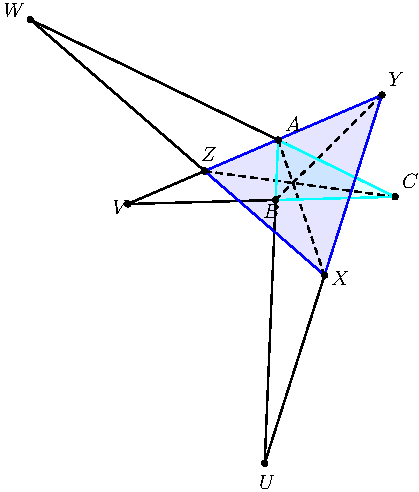
\includegraphics{desargues.pdf}
	\caption{The Desargues' Theorem}
\end{figure}


\section{Pascal's Theorem}
\begin{theorem}[Pascal's Theorem]
If hexagon $ABCDEF$ lies on a circle then $AB\cap DE=X, BC\cap EF =Y, CD\cap FA=Z$ are collinear.
\end{theorem}

\begin{figure}[ht]
\centering
	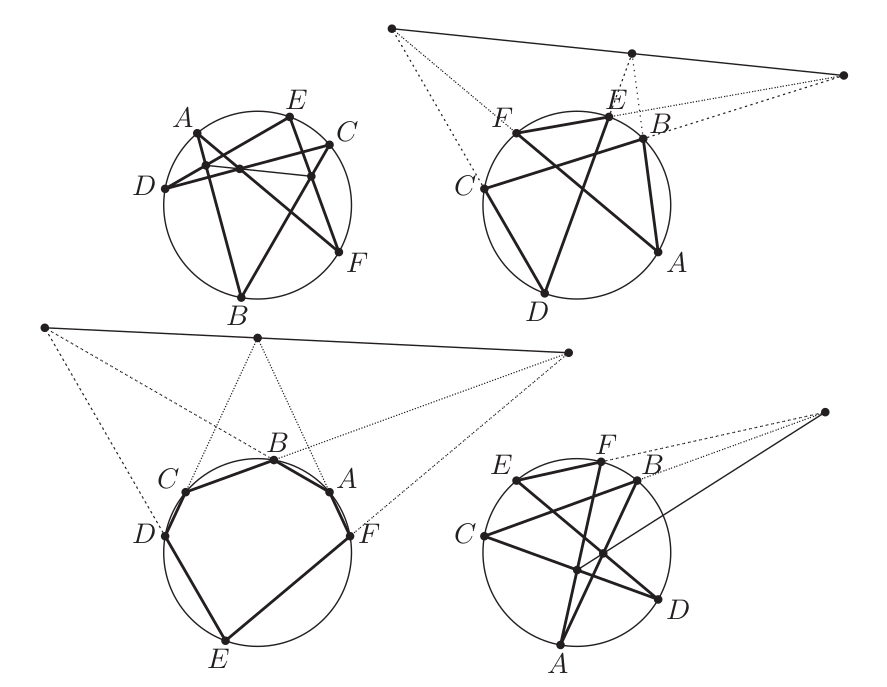
\includegraphics[scale=0.3]{pascals.png}
	\caption{Many Faces of Pascal's Theorem (adapted from Evan Chen's EGMO)}
\end{figure}

\begin{remark*}
If $X,Y,Z$ are collinear then you can not say that $ABCDEF$ lies on a circle.
\end{remark*}
Pascal's Theorem is most useful of these five theorem. It can be applied to as well as triangles, quadrilaterals and pentagons.
Where as an example we apply Pascal's on $AABBCC$ we get $AA\cap BC $ $AB \cap CC$ and $BB \cap CA$ are collinear where $AA$ means the tangent to the circumcircle at $A$, and so on.

So, it seems very useful in different problems containing triangles, quadrilaterals, pentagons and hexagons.


\section{Pappu's theorem}
\begin{theorem}[Pappu's Theorem]
$A,B,C,D,E,F$ are six poins on the plane. Let $AB\cap DE=X, BC\cap EF =Y, CD\cap FA=Z$. Then, $A,C,E$ and $B,D,F$ are collinear if and only if $X,Y,Z$ are collinear.
\end{theorem}
You may wonder that, Problem 2 of IMO 2019 can be solved using Pappu's Theorem along with some other facts.
\begin{figure}[ht]
\centering
	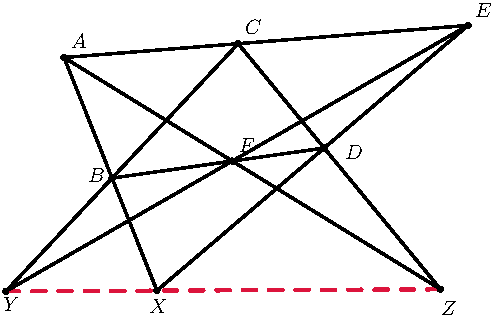
\includegraphics{pappu.pdf}
	\caption{Pappu's Theorem}
\end{figure}

\section{Brianchon's Theorem}
\begin{theorem}[Brianchon's Theorem]
$ABCDEF$ is a tangential hexagon (i.e. Sides of the hexagon are externally tangent to a common circle). Then, $AD,BE,CF$ are concurrent.
\end{theorem}
Brianchon's Theorem can be derived directly from Pascal's Theorem by only interchanging the words 'points' and 'line', and making whatever
grammatical adjustments that are necessary.

Brianchon's and Pascal's theorem form Pole Polar duality of Projective Geometry. 
\begin{figure}[ht]
\centering
	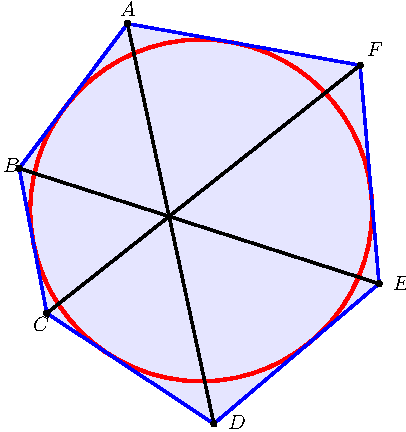
\includegraphics{brianchon.pdf}
	\caption{Brianchon's Theorem}
\end{figure}
Point to be noted that, we can take $C,D,E$ collinear, then the polygon becomes a pentagon. We also can take $A,B,C$ and $D,E,F$ collinear, then the polygon becomes a tangential quadrilateral.
Here, $B,E$ become point of tangency. Let, $CD$ and $FA$ touches the circle at $G,H$ then, $AD,CF,BE,GH$ all are concurrent.

\begin{figure}[htt]
\centering
	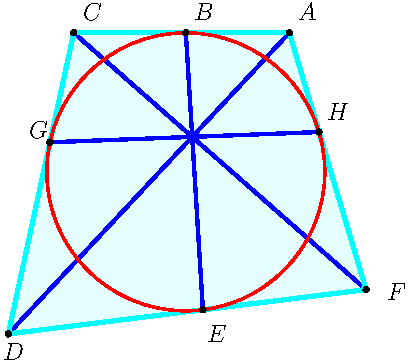
\includegraphics[scale=1]{brian-quad.pdf}
	\caption{Brianchon's Theorem on a quadrilateral.}
\end{figure}

\section{Butterfly Theorem}
\begin{theorem}[Butterfly Theorem]
$AB$ be a chord of a circle with midpoint $M$. Let two chords through $M$ of the circle are $CD$ and $EF$. $CE\cap AB=X$ and $DF\cap AB=Y$. Then, $MX=MY$. 
\end{theorem}
%The converse is also true for Butterfly Theorem. If $
\begin{figure}[ht]
\centering
	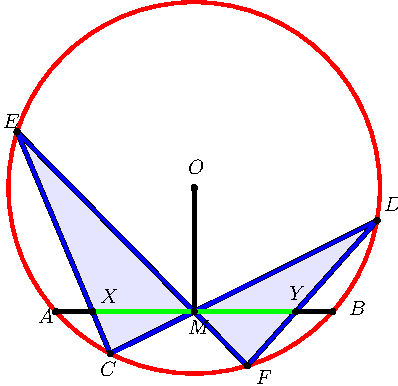
\includegraphics{butterfly.pdf}
	\caption{The butterfly theorem, look polygon $CEFD$ looks like a butterfly!}
\end{figure}


The Theorem is also tru if the chord is not a chord of the circle i.e. the line lies outside the circle, as the next theorem says.




\begin{theorem}[Extended Butterfly Theorem]
Let $\ell$ be a line on the plane of a circle $\omega$. $O$ is the center of the circle. Let $M$ be a point on $\ell$ such that $OM\perp \ell$. Let two lines through $M$ intersects the circle at $C,E$ and $D,F$ respectively. Let $DE$ and $CF$ meet $\ell$ at $B,A$ respectively. And $CD$ and $EF$ meet $\ell$ at $H,G$ respectively. Now, $AM=BM$ and $GM=HM$.
%----------
%$AB$ be a chord of a circle with midpoint $M$. Let two chords through $M$ of the circle are $CD$ and $EF$. $CE\cap AB=X$ and $DF\cap AB=Y$. Then, $MX=MY$. 
\end{theorem}

\begin{figure}[ht]
\centering
	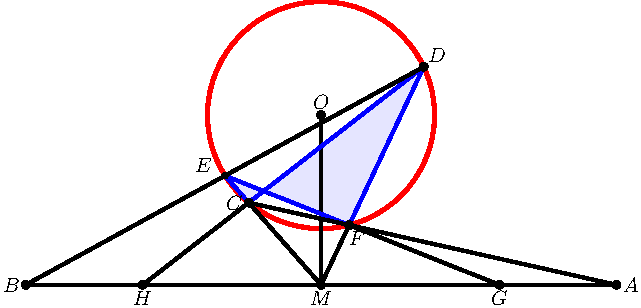
\includegraphics{butterfly-extended.pdf}
	\caption{Extended Butterfly Theorem}
\end{figure}

\section{Practise Problems}


\begin{problem}


	\begin{hint}
	\addhint{}
	\addhint{}
	\end{hint}
\end{problem}

\begin{problem}


	\begin{hint}
	\addhint{}
	\addhint{}
	\end{hint}
\end{problem}

\begin{problem}


	\begin{hint}
	\addhint{}
	\addhint{}
	\end{hint}
\end{problem}

\begin{problem}


	\begin{hint}
	\addhint{}
	\addhint{}
	\end{hint}
\end{problem}

\begin{problem}


	\begin{hint}
	\addhint{}
	\addhint{}
	\end{hint}
\end{problem}

\begin{problem}


	\begin{hint}
	\addhint{}
	\addhint{}
	\end{hint}
\end{problem}

\begin{problem}


	\begin{hint}
	\addhint{}
	\addhint{}
	\end{hint}
\end{problem}

\chapter{Lifting The Exponent (LTE) Lemma}% by Tanmoy Sarkar}
\begin{linkb}
   \begin{itemize}
        \item \href{https://www.youtube.com/watch?v=D7Pt_mROJcw}{Lifting The Exponent (Tanmoy)}
        \item \href{https://drive.google.com/file/d/1en-kqZcoNRirudjEO_iTA67T6MgCBGPi/view}{LTE} 
   \end{itemize}
\end{linkb}
\section{Definitions and the Lemma}

We previously discussed about the p-adic valuation function $\upsilon_p(m)$ of a positive integer $m$ for which $\upsilon_p(m)$ is the highest power of a integer $p$ that divides  $m$

\begin{lemma}
 For $x,y \in \mathbb{Z}$ and  $n \in \mathbb{N}$, let $P$ be a odd prime number such that $(n,p)=1$ , $p\nmid x, y$ but $p|x-y$, then $$\upsilon_(x^n-y^n)=\upsilon_(x-y)$$
\end{lemma}

\textbf{Proof:} Given that $$x-y \equiv  0 \pmod p$$ $$\implies x \equiv y \pmod p$$ $$\implies x^{n-1} \equiv y^{n-1} \pmod p$$ $$\implies x^{n-2}y \equiv y^{n-1} \pmod p$$  $$\implies x^{n-3}y^2 \equiv y^{n-1} \pmod p$$ and so  goes on.

But $$x^n-y^n=(x-y)(x^{n-1}+ x^{n-2}y+x^{n-3}y^2+.....+xy^{n-2}+y^{n-1})$$
$$x^n-y^n=(x-y)(ny^{n-1}) \pmod p$$
But as $p \nmid n, y$, so,  $\upsilon_(x^n-y^n)=\upsilon_(x-y)$ 

\begin{lemma}
 For $x,y \in \mathbb{Z}$ and  $n \in \mathbb{N}$ and $n$ even, let $P$ be a odd prime number such that $(n,p)=1$ , $p\nmid x, y$ but $p|x+y$, then $$\upsilon_(x^n+y^n)=\upsilon_(x+y)$$
\end{lemma}
\textbf{Proof:} The proof is similar to the previous one.

\begin{theorem} [Lifting the exponent lemma]
Let $p$ be an odd prime and let $\nu_p(n)$
	be the exponent of $p$ in the prime factorization of $n$.
	If $a \equiv b \not\equiv 0 \pmod p$ then
	$\nu_p(a^n-b^n) = \nu_p(n) + \nu_p(a-b)$.

\end{theorem}

\section{Example Problems}
\begin{example}
Given that $2^p+3^p=a^n$ for prime $p$ and positive integer $a$, prove that $n=1$
\end{example}

We see that 2+3=5; so taking $\upsilon_5$ we get,
$$\upsilon_5(2^p+3^p)=\upsilon_5(2+3)+\upsilon_5(p)$$
$$\implies \upsilon_5(2^p+3^p)=1+0=1$$

so, $$\upsilon_5 (a^n)=1=n\upsilon_5(a)$$
Hence $n=1$

\begin{example}
Prove that there exists infinitely many positive integers $n$ such that $n|2^n+3^n$
\end{example}
We take $n=5^k$ for positive integers $k$, we want to show that $5^k|2^{5^k}+3^{5^k}$

From LTE, we show that $$\upsilon_5(2^{5^k}+3^{5^k})=\upsilon_5(2+3)+\upsilon_5(5^k)$$
$$\implies \upsilon_5(2^{5^k}+3^{5^k})=1+k$$
so, $5^{k+1}|2^{5^k}+3^{5^k} \implies 5^{k}|2^{5^k}+3^{5^k}$

Hence there exists infinitely many positive integers $n$ of form $5^k$ that divides $a^n+b^n$

\begin{example}
Given that $a^p \equiv 1 \pmod {p^n}$ for prime $p$, prove that $a^p \equiv 1 \pmod {p^{n-1}}$
\end{example}

\begin{example}
$2^m-3^n=1$ and $m,n \in \mathbb{N}$, find $m,n$.
\end{example}
\section{Practise Problems}

\chapter{Combinatorial Algebra}% by Rafi Mahmud}

\begin{linkb}
   \begin{itemize}
        \item \href{https://www.youtube.com/watch?v=jFvk-na3WC0}{Combinatorial Algebra (Rafi)}
       % \item 
   \end{itemize}
\end{linkb}

\section{What is this?}


\section{Example Problems}


\section{Practise Problems}



%%%%%%%%%%%%%%%%%%%%%%%
%\chapter{May 6, 2021}
\chapter{Number Theory TSTST}\label{tstst:nt}
%National camp Exam 1

%:%'(
The Number Theory Exam of The National Camp.
Problems are given below:
\begin{prob}\label{nt:1}
Let $N$ be an integer. Given any $a, b$ such that $\gcd(a, b, N) = 1$. Prove
that you can find $m, n$ such that $(m, n) = 1$ and $N\mid m - a, N\mid n - b$.
\end{prob}

\begin{prob}\label{nt:2}
Let $p$ be a prime number. We call a subset $S$ of $\{1, 2, \ldots , p - 1\}$
“good” if it satisfies the property that for every $x, y \in S$, $xy \pmod p$ is also in $S$.
How many “good” sets are there?
\end{prob}

\begin{prob}\label{nt:3}
Let $P(x)$ be a nonzero integer polynomial, that is, the coefficients
are all integers. We call a prime $q$ “interesting” if there exists some natural
number $n$ for which $q|2^n + P(n)$. Prove that there exist infinitely many “iner-
esting” primes.
\end{prob}



Full Solutions to these problems can be found at \autoref{sols:tstst}.

\newcommand{\astt}{^{\ast}}

\chapter{Inversive \& Projective Geometry}% by Saad Bin Quddus}

\begin{linkb}
   \begin{itemize}
        \item \href{https://www.youtube.com/watch?v=P4FN_-LOEx4}{Projective Geometry (Saad)}
        \item \href{https://drive.google.com/file/d/1MfmQFOs-N120PnhCfIheByLBQKbua9Jl/view}{1}, \href{https://drive.google.com/file/d/14VtTlUP3GvV1vjV_Njt5o0TbSzBvfE0-/view}{2}
   \end{itemize}
\end{linkb}

\section{Inversion}
An inversion wrt a circle send a point($A$) inside to a point($A\astt$) outside the circle such that $OA\cdot OA\astt =r^2$,
where $r$ is the radius of the circle.
\begin{figure}[ht]
\centering
	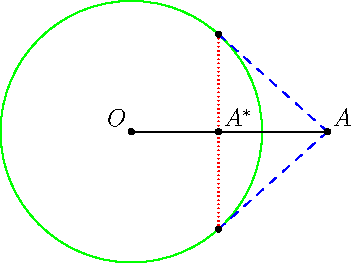
\includegraphics[scale=1]{tangent.pdf}%{inverse-a.png}
	\caption{$A\astt$ is the inverse of $A$ with respect to $\omega$.}
\end{figure}
Remember that $O,A,A\astt$ lie on a line but $O$ doesn't lie between $A$ and $A\astt$.

An interesting result about inversion is if $A\astt, B\astt$ are the inverse of $A,B$ respectively then $A,B,B\astt, A\astt$ are concyclic.
\begin{figure}[h!t]
\centering
	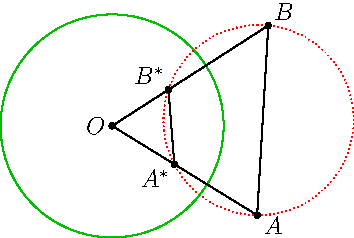
\includegraphics[scale=1]{inv-cyclic.pdf}%{inverse-cyclic.png}
	\caption{A cyclic quadrilateral}
\end{figure}


Inverse of a circle with respect to circle $\omega$ (intersecting $\omega$ at $A,B$) is a line through $A,B$.

Remember that the inverse of the center with respect to $\omega$ is a point at infinity.

\begin{figure}[h!t]
\centering
	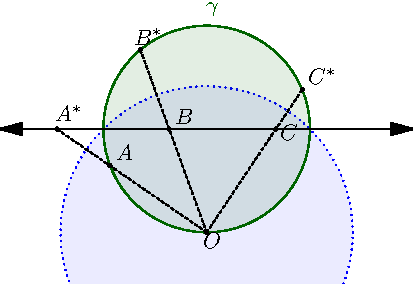
\includegraphics[scale=1]{inverse-cline.pdf}%{inverse-cline.png}
	\caption{A circle inverts to a line and vice-versa}
\end{figure}
Also another fact that two circle orthogonal to each other are overlaying with respect to the other circle.

\section{Projective Geometry}
\begin{theorem}[La Hire's Theorem]
A point $X$ lies on the polar of a point $Y$ if and only if $Y$ lies on the polar of $X$.
\end{theorem}

\paragraph{Harmonic Division}
Let four points $A,C,B,D$ lie on a line in that order. These points are called harmonic if $\frac{AC}{BC} \div \frac{AD}{BD} =-1$ where the lengths are directed.
And denoted by $(A,B;C,D)=-1$ 

We can solve lots of problems with this, litteraly.

\paragraph{Pencil}
Let four collinear points are $A,B,C,D$ and another line $\ell$. An another point(not neccessarily distinct) $P$. Line through $P$ connecting $A,B,C,D$ intersects $ell$ at $A',B',C',D'$ respectively. Then 
\[(A,B;C,D)=(A',B';C',D')\]
So their cross ratio remain same!

\begin{lemma}[Cevian Induces Harmonic Bundle]
Let $AD,BE,CF$ are concurrent cevians, $EF\cap BC=G$ then, $(B,C;D,G)=-1$
\end{lemma}

\begin{figure}[h!t]
\centering
	\includegraphics[scale=1]{cevian-harmonic.pdf}
	\caption{$B,C,D,G$ is a harmonic bundle.}
\end{figure}
You can prove the above lemma using just Ceva's and Menelaus's Theorem.
Note that, $AX,BY,CZ$ are concurrent hence, follows Ceva's Theorem and $E,F,G$ are collinear following Menelaus's Theorem.



\begin{lemma}[Complete Quadrilaterals Induces Harmonic Bundles] \label{lemma:com-har}
Let ABCD be 
a quadrilateral whose diagonals meet at $K$. Lines $AD$
 and $BC$ meet at $L$, and line $KL$ 
meets $AB$ and $CD$ at $M$ and $N$ . Then $(K, L; M, N)$
 is a harmonic bundle. 
\end{lemma}

\begin{figure}[h!t]
\centering
	\includegraphics[scale=1]{complete-quad-harmonic.pdf}
	\caption{$K,L,M,N$ is also a harmonic bundle.}
\end{figure}

Let $AB$ and $CD$ inersect at $P$ and $PK$ and $BC$ intersect at $Q$, then, $(Q,L,B,C)=-1$ and projecting onto the desired line through $P$ gives us the result.

Now, you can solve a problem using the results we have derived above.

\begin{example}[USA TST 2011/1]
In an acute scalene triangle $ABC$, points $D, E, 
F$ lie on sides $BC, CA, AB,$ respectively, such that $AD \perp BC, BE \perp CA, CF \perp AB$.
Altitudes $AD, BE, CF$ meet at orthocenter $H$. 
Points $P$ and $Q$ lie on segment $EF$ such that 
$AP \perp EF$ and $H Q \perp EF$ . Lines $DP$ and $QH$  intersect 
at point $R$. Compute $HQ/HR$.
\end{example}

By using \autoref{lemma:com-har},  we can derive that,  
$(A,H; AD \cap EF , D)=-1$, and projecting through $P$
 gives  $(P_{\infty}, H ; Q, R)=-1$ where $P_{\infty}$
 is the point at infinity on parallel lines $AP$ and
  $QR$ Hence, $HQ/HR=1$.

\begin{lemma}[Midpoints and Parralel Lines]
Given points $A$ and $B$, let $M$ be the
midpoint of $AB$ and $P_{\infty}$ the point at infinity of line $AB$. Then $(A, B; M, P_{\infty})$ is a harmonic bundle.
\end{lemma}

\begin{proposition}[Harmonic Quadrilateral]
$ABCD$ cyclic quadrilateral and $AC/BC = AD/BD$ then $ABCD$ is called harmonic quadrilateral.
\end{proposition}
\begin{figure}[h!t]
\centering
	\includegraphics[scale=1]{har-quad.pdf}%{harmonic-quad.png}
	\caption{Here $AXBY$ is a harmonic quadrilateral}
\end{figure}
Harmonic Quadrilateral has many nice and cute properties:
\begin{enumerate}[{\textbf (a)}]
	\ii If tangent at $B$ and $D$ meet at $T$ then, $A,C,T$ are collinear. The intersection of the diagonals ($S$) is also collinear with $A,C,T$.
	\ii $S$ and $T$ are inverse of each other with respect to $(ABCD)$.
	\ii $AC$ is an $A$-Symmedian of $DAB$ and $C$-Symmedian of $BCD$. Analogous for $BC$.
\end{enumerate}


\begin{lemma}[Right Angles and Bisectors]
Let $X,A,Y,B$ be collinear points in that order and let $C$ be any point not on this line. Then any two of the following conditions implies the third condition.
\begin{enumerate}[i]
	\ii $(A,B;X,Y)$ is a harmonic bundle.
	\ii $\angle XCY=90\dg$.
	\ii $CY$ bisects $\angle ACB$.
\end{enumerate}
\end{lemma}

\begin{figure}[h!t]
\centering
	\includegraphics[scale=1]{right-bisector.pdf}%{right-angles-bisector.png}
	\caption{$CX$ and $CY$ are external and internal angle bisectors.}
\end{figure}

\begin{lemma}[Midpoint of a Segment]
$(A,B,C,D)=-1$ and $M$ is the midpoint of $AB$, then 
\begin{itemize}
	\ii $MA^2=MB^2=MC\cdot MD$.
	\ii $DA\cdot DB = DC \cdot DM$.
\end{itemize}
\end{lemma}


\begin{theorem}[Brocard's Theorem]
Let $ABCD$ be an arbitrary cyclic quadrilateral
inscribed in a circle with center $O$, and set $P = AB \cap CD, Q = BC \cap DA, \text{and } R =
AC \cap BD.$ Then $P , Q, R$ are the poles of $QR, RP , P Q$, respectively.
In particular, $O$ is the orthocenter of triangle $PQR$.
\end{theorem}
\begin{figure}[h!t]
\centering
	\includegraphics{brocard.pdf}
	\caption{$(OAMC)$ and $(OBMD)$ are the inverses of $AC$ and $BD$ respectively.}
\end{figure}

Here we see that $R$ is the inverse of $M$. So, $O,R,M$ are collinear. 

And consequently, $PQ$ is the polar of $R$.

We shall prove that $PR$ is polar of $Q$ and $QR$ is polar of $P$.

$Q,R\in \text{ polar of }P$
So, we have from La Hire's Theorem that $P$ belongs to polar of both $Q,R$.

Then, join $Q,R$ and they intersect the circle and $AB,CD$ at four points and then doing some harmonic bundle chase gives the desired result and left as an exercise!

\section{Practice Problems}


\begin{problem}


	\begin{hint}
	\addhint{}
	\addhint{}
	\end{hint}
\end{problem}

\begin{problem}


	\begin{hint}
	\addhint{}
	\addhint{}
	\end{hint}
\end{problem}

\begin{problem}


	\begin{hint}
	\addhint{}
	\addhint{}
	\end{hint}
\end{problem}

\begin{problem}


	\begin{hint}
	\addhint{}
	\addhint{}
	\end{hint}
\end{problem}

\begin{problem}


	\begin{hint}
	\addhint{}
	\addhint{}
	\end{hint}
\end{problem}

\begin{problem}


	\begin{hint}
	\addhint{}
	\addhint{}
	\end{hint}
\end{problem}

\begin{problem}


	\begin{hint}
	\addhint{}
	\addhint{}
	\end{hint}
\end{problem}
%\section{}

\chapter{Algorithms}% by Ahsan Al Mahir}

\begin{linkb}
   \begin{itemize}
        \item \href{https://www.youtube.com/watch?v=VjXhzp-hYoE}{Algorithms (Lazim)} 
        \item \href{https://drive.google.com/file/d/1p0i6hqSbMrBuEjdoiQCPlfXQlBMAtMJ3/view}{Class}, \href{https://drive.google.com/file/d/1KeTtY-0IxhPWDcDFvvau15P9_OEyCuq_/view}{Note}
   \end{itemize}
\end{linkb}

(We followed the note \textit{Algorithms} by Cody Johnson from France IMO Training Camp 2015. This note is a great resource for further reading.)
An algorithm is a set of steps to perform a procedure.

You may know the \textbf{Binary Search Algorithm}.(the number guessing game is a game
in which your opponent thinks of a integer $n$ on an interval $[a, b]$, and you try to guess his number with the
rule that after every guess he must tell you if your guess was correct, too high, or too low. you can win this game by at most $\log_2(b-a+1)$ guesses.)

\section{Greedy Algorithms}
The greedy algorithm is an algorithm that chooses the optimal choice in the short run.
It arises naturally. 
You can solve many of the problems appear in various olympiads by greedy-approch.


\begin{example}[Binary Number System]
Prove that every positive integer can be written uniquely as
the sum of one or more distinct powers of $2$.
\end{example}
Here, we take the highest power of $2$ (say $m$) less than or equal to the integer $n$. Then, apply the algorithm to the number $(n-m)$.
And consequntly we are done! (by strong induction)


\begin{example}[Zeckendorf's Theorem]
Prove that every positive integer can be written uniquely as
the sum of one or more Fibonacci numbers, no two of which are consecutive Fibonacci numbers.
\end{example}
Here, work similarly a sthe above example, lsrgest power of $2$ replaced by the largest Fibonacci number less than or equal to $n$.


Here, we comes to a graph coloring problem. 
Algorithms are hugely applied in graph 
theoretic problems especially in graph coloring.

\begin{example}
Let $\Delta$ be the maximum degree of the vertices of a given graph. Devise a method to
color this graph using at most $\Delta + 1$ colors such that no two neighboring vertices are of the same color.
\end{example}
We shall use the following greedy algorithm: for each vertex, we shall color it with any color that has
not been used by any of its neighbors. Since each vertex has at most $\Delta$ neighbors, at least one of the $\Delta + 1$
colors has not been used, so such a color will always exist. Thus, we are done.



\section{Reduction Algorithms}
Algorithms can be used to reduce a complex configuration to a simple one while preserving its combinatorial
function in the problem.
\begin{example}[Cody Johnson]
Consider an ordered set $S$ of $6$ integers. A move is defined by the
following rule: for each element of $S$, add either $1$ or $-1$ to it. Show that there exists a finite sequence
of moves such that the elements of the resulting set, $S' = (n_1 , n_2 , \ldots , n_6)$, satisfy $n_1 n_5 n_6 = n_2 n_4 n_6 =
n_3 n_4 n_5$.
\end{example}
Here show that, we can reduce all the elements to noly $0$ and $1$. Now it is easy to tackle the problem. Then you can assume for the sake of contradiction that the products are not equal. After this some case works solve the problem.



\begin{example}[Canada MO]
Let $n\times n$ be grid of squares. Their is some barricades such that none of the squares are isolated. There is two robots arbitrarily placed on two square. You can perform up, down, left, right commands to control the robots but it is simutaneous. Prove that it is possible to take 2 robots at the lower left corner of the grid. 
\end{example}

Here are two ideas to solve it.

First one is to take the robot which is furthest from the lower left square, then take it to the rquired square. And then the other.

Another approach is to show that, we can restrict (or take) two robots at a single square sometime. Then we are done by giving the commands U,R,L,D.

\section{Invariant and Monovariant}
See \nameref{sec:inv-mono}. This class covered invariants and mnonovariants.




\chapter{Recursion}% by Mursalin Habib}

\begin{linkb}
   \begin{itemize}
        \item \href{https://www.youtube.com/watch?v=Jh8VFmv5_s4}{Solving Recurrence }
        %\item 
   \end{itemize}
\end{linkb}
%\section{solving Recurrences}
\section{Definitions}
A \textbf{Recurrence} sequence is a type of sequence where the following terms of the sequence depends on the previous terms of the sequence.

$$A_n=A_{n-1}+A_{n-2}-3A_{n-3}$$ is a recurrence relation where every term depends on it previous three terms.

A \textbf{linearly recurrence sequence} is a recurrence where the relation with the following term and the previous terms is linear(or has a power of 1). The previously mentioned recurrence sequence is a linear recurrence sequence.

The common structure of a \textbf{homogeneous linearly recurrence sequence} is $$T_n=C_1T_{n-1}+C_2T_{n-2}+C_3T_{n-3}+...+C_{k-1}T_{n-k+1}+C_kT_{n-k}$$, where $k$ is a positive integer less than $n$ and greater than $0$.

\section{Solving Recurrence}
\begin{example}
Solve the recurrence $$T_n=5T_{n-1}-6T_{n-2}$$
\end{example}
$$T_n=C_1T_{n-1}+C_2T_{n-2}+C_3T_{n-3}+...+C_{k-1}T_{n-k+1}+C_kT_{n-k}$$ here, the \textbf{order} of this recurrence is $k$.

So, in our following problem, the order is 2.

To, solve the recurrence, first we have the find the \textbf{characteristic polynomial} of the recurrence.

The characteristic polynomial of $$T_n=C_1T_{n-1}+C_2T_{n-2}+C_3T_{n-3}+...+C_{k-1}T_{n-k+1}+C_kT_{n-k}$$ would be $$x^k-c_1x^{k-1}-c_2x^{k-2}-....-c_kx^{0}=0$$
%\section{Example Problems}


\section{Practise Problems}


%%%%%%%%%%%%%%%%%%%%%%%
%\chapter{May 9, 2021}
\chapter{Geometry TSTST}\label{tstst:geo}
%National camp Exam 2
%:'(
The Geometry Exam of The National Camp.
%Question
Problems are given below:

\begin{prob}\label{geo:1}
Let $\triangle ABC$ be a triangle inscribed in a circle $\omega$. $D, E$ are two points on the arc $BC$
of $\omega$ not containing $A$. Points $F, G$ lie on $BC$ such that
\[\angle BAF =\angle CAD %\mathrm{and} 
\text{ and } \angle BAG=\angle CAE\]
Prove that the two lines $DG$ and $EF$ meet on $\omega$.
\end{prob}

\begin{prob}\label{geo:2}
$ABC$ is a triangle where $\angle BAC = 90\dg$ . A line through the midpoint $D$ of $BC$ meets
$AB$ at $X$ and $AC$ at $Y$ . The point $P$ is taken on $XY$ such that $PD$ and $XY$ have the same midpoint
$M$. The perpendicular from $P$ to $BC$ meets $BC$ at $T$ .

Prove that AM bisects $\angle TAD$.
\end{prob}

\begin{prob}\label{geo:3}
Let $ABC$ be a triangle with $BC$ being the longest side. Let $O$ be the circumcenter
of $ABC$. $P$ is an arbitrary point on $BC$. The perpendicular bisector of $BP$ meet $AB$ at $Q$ and the
perpendicular bisector of $PC$ meet $AC$ at $R$. Prove that $AQOR$ is cyclic.
\end{prob}

\textit{After solving all of the three problems above, you may try this bonus problem. Beware though,
any work done on Problem 4 with incomplete solutions of the first three won’t receive any
points.}

\begin{prob}\label{geo:4}
Let $ABC$ be a triangle with circumcircle $(O)$. The midpoints of $BC,CA, AB$ are
$A', B', C'$ respectively. The medians $AA', BB' ,CC'$ cut the circumcircle $(O)$ at $A, A_1 ; B, B_1 ; C,C_1$
respectively. The line of tangency to $(O)$ at $A_1$ meets the perpendicular to $AO$ through $A ′$ at $X$.
Define $Y, Z$ similarly. Prove that $X,Y, Z$ are collinear.
\end{prob}



Full Solutions to these problems can be found at \autoref{sols:tstst}.

%\pagebreak



%------------------------
%\part{Special Chapters}

%\input{tex/gametheory.tex}
%\input{tex/coloring.tex}
%\input{tex/probability.tex}
%\input{tex/specialgeo.tex}



%------------------------
%\backmatter
\appendix
\chapter{Hints to Selected Problems}
\makehints
\makehintss


\chapter{Solutions to BGD TSTST Problems}\label{sols:tstst}


\section{Solutions to \nameref{tstst:combi}}

\subsection*{Solution to \autoref{combi:1}}
\paragraph{First Solution (Mehrab, unedited)}
Let us assume that there is no circle with a radius of 1  unit which has more than 9  points from S  in it. Now let us take the leftmost point of S  in the plane and take it as a centre and draw a circle of radius 1 . Now at most 8 other points can be inside the circle. That means there are at least 10  other points outside the circle. Now again take the left most of the points outside the circle we have just drawn. And we now draw another circle with a radius 1  with that point as the centre. The new circle can have at most 8 points that are not present in our first circle. So now we have a point in S  that are not in any of the 2 circles we have drawn. But If we take that rogue point and the centre of the 2 circles then 2 points of those 3 must have a distance less than 1  meaning the rogue point should be inside any one of the 2 circles. A contradiction. 


\paragraph{Second Solution (Nayer,unedited)}
Let $G$ be a graph with $19$ vertices and by an edge between any two vertices we mean that they are less than. 1 unit apart.

Let $G'$ be the complement of the graph $G$. Then that means in $G'$, an edge between any two points means that they are At least $1$ unit apart. Now ATQ there cannot be any clique of size $3$  in $G'$ (otherwise that would imply that we would get a triangle in
$G$ with no edge which is impossible)

So, By Turan's theorem, $G'$ can have at most $\frac{1}{2}\times \frac{19^2}{2} \sim 90 $ edges. That means $G$ has $\binom{19}{2}−90 =81$  edges.

By handshake lemma, sum of degree of vertices $\ge 81\times 2=162$. 

By pigeonhole principle there must exist a vertex in G with at least degree $\frac{162}{19} \sim 9$

WLOG suppose that vertex is $V$ Now draw a circle with radius $1$ with centre $V$. So at least $9$ other points are enclosed by that circle.

\subsection*{Solution to \autoref{combi:2}}

\subsection*{Solution to \autoref{combi:3}}


\subsection*{Solution to \autoref{combi:4}}

\subsection*{Solution to \autoref{combi:5}}
%(Solution from Olympiad Combinatorics)
Suppose we have an empty board, and we want to create an arrangement of $k$ checkers satisfying (a) and (b). Call a square good if it contains a checker or shares a side with a square containing a checker. By (a), every square must eventually be good. Let us place the checkers on the board as follows: place one checker on the board to start, and then in each step place one checker adjacent to one that has already been placed. Since any arrangement of checkers that satisfies the problem must be connected by (b), we can form any arrangement of checkers in this manner. 

In the first step at most 5 squares become good (the square we placed the checker on and its neighbors). In each subsequent step, at most 3 squares that are not already good become good: the square we just put a checker on and the square next to it are already good, leaving 3 neighbors that could become good. Thus, at the end of placing k checkers, at most $5+3(k-2) = 3k+2$ squares  are good. But we know all $n^2$ squares are good at the end, so $n \le 3k+2$, proving the result.








\section{Solutions to \nameref{tstst:nt}}


\subsection*{Solution to \autoref{nt:1}}

\subsection*{Solution to \autoref{nt:2}}


\subsection*{Solution to \autoref{nt:3}}







\section{Solutions to \nameref{tstst:geo}}

\subsection*{Solution to \autoref{geo:1}}

\begin{figure}[ht]
\centering
	\includegraphics{geo-1.pdf}
\end{figure}
First of all, there are tons of similar triangles. You should find them. We left the angle chasing for the readers as these are good  exercises. 

Note that, $\triangle CAG$ and $\triangle EAB$ is directly similar. Hence, 
\[ AE \cdot AG = AB \cdot AC \ldots (1) \]

Then show that, $\triangle BAF$ and $\triangle DAC$ are similar. So, 
\[ AD \cdot AF = AB \cdot AC \ldots (2)  \]
From (1) and (2) we get, 
\[  AE \cdot AG = AD \cdot AF \ldots (3) \]
So, $\triangle AEF \sim \triangle ADG$. 
Hence, $\angle AEF = \angle ADG.$

Then, we get $\triangle EAD \sim \triangle FAG.$ 

After some angle chase (left as an exercise) we  get the result that, $\angle EZD = \angle EAD$, and therefore $Z$ lies on the  circle.

\subsection*{Solution to \autoref{geo:2}}

\begin{figure}[ht]
\centering
	\includegraphics{geo-2.pdf}
\end{figure}

$BD=CD=AD$ ,
$MX=MA=MY$ and
$MD=MP=MT$ 
as $\triangle PTD$ is right angled.
So, $\angle MDT=\angle MTD$
$= \angle BDX = 180 -\angle BXD - \angle DBX =180 - (\angle BAY +\angle AYX ) - \angle DAB $
$=180 -(90+\angle MAC)- \angle DAB =90 -(\angle MAC + \angle DAB)$
 $\boxed{= \angle DAM =\angle DTM} $
$\implies ADMT $ is cyclic. hence $\angle MDT =\angle MTD $
$\implies \angle MAT =\angle MAD$ which implies $AM$ bisects the desired angle. 

\subsection*{Solution to \autoref{geo:3}}
\begin{figure}[ht]
\centering
	\includegraphics{geo-3.pdf}
\end{figure}

Let $P'$ be the reflection of $P$ over $QR$.
then, $QP=QP'=QB$ and 
$RP=RP'=RC$
$\angle RP'Q=\angle QPR=180 -\angle B -\angle C=\angle A$
So, $PQP'A$ is cyclic.
So,$\angle P'QA=\angle P'RA$, and $P'Q=BQ$, $P'R=CR$.
So, $\triangle P'QB,  \triangle P'RC$ are similar.
Hence $$\angle P'BA= \angle P'BQ=\angle P'CR=\angle P'CR=\angle P'CA$$.
Which results in $BPCA$ is cyclic.
Now $$\angle P'OQ=\frac{1}{2} P'OB=\angle P'CB=\angle P'AB=\angle P'AQ=\angle P'RQ$$
Hence $P'QOR$ is cyclic. we proved $P'QRA$ cyclic before. 
So $AQOR$ is cyclic.


\subsection*{Solution to \autoref{geo:4}}
\begin{figure}[htb]
\centering
	\includegraphics[scale=.8]{geo-4.pdf}
\end{figure}
Solution thanks to Luis Gonz\'{a}lez.

Centroid $G = AA' \cap BB' \cap CC'$ of $\triangle ABC$ is the insimilicenter between its circumcircle $(O)$ and $9$-point circle $(N)$. $A, A'$ are homologous under such homothety implies tangent $\nu$ of $(N)$ at $A'$ is parallel to the tangent $\tau$ of $(O)$ at $A$. Which implies $\nu$ is antiparallel to $BC$ $\implies  A'X \equiv \nu$. The lines $\tau, XA_1$ and $AA_1$ bound an isosceles triangle, therefore $\triangle XA'A_1$ is isosceles with apex $X$ implies $X$ has equal power with respect to $(O)$, $(N)$. Which implies $X$ lies on the radical axis of $(O), (N)$, i.e. the orthic axis of $\triangle ABC$. Analogously, $Y, Z$ lie on the orthic axis of $\triangle ABC$.



\end{document}
